% !TeX encoding = UTF-8
% 此文件从2021.8开始

\chapter{微分流形}\label{chdm}
本章将介绍微分流形概念,这是微分几何的基础.
接着介绍流形上的切矢量场、余切矢量场、张量场,
然后叙述单参数变换群以及李导数.


本章及以后各章节,如无特殊声明,在实数域$\mathbb{R}$上讨论问题.


\section{平直的广义欧几里得空间}\label{chdm:sec_Euclidean-space}
在正式描述弯曲的(指黎曼曲率非零)微分流形前,
再对平直的(指黎曼曲率为零)广义欧几里得空间做些说明是大有裨益的.
本节的概念可直接用到流形上的切空间,进而可用到流形论中.
本节是连接上一章与微分流形的桥梁.
欧氏空间的定义见\pageref{chmla:def_Euclidean-space}页\ref{chmla:def_Euclidean-space},
它就是指定了正定度规($g(\cdot,\cdot)\equiv \left<\cdot,\cdot\right>$)的矢量空间.


\subsection{定义}\label{chdm:sec_gen-Euclidean-space}

\begin{definition}\label{chdm:def_MinkowskiSpace}
    设$V$是实数域$\mathbb{R}$上的$m$维线性空间,
    给定$V$上{\uwave{非退化的}、\uwave{对称的}}双线性
    函数$g(\cdot,\cdot)\equiv \left<\cdot,\cdot\right>$,那么$V$称为{\heiti 广义欧几里得空间},
    记为$(V,g)$.
    
    若在\S \ref{chmla:sec_sbf}的式\eqref{chmla:eqn_gmetric}中全是正号,
    则此空间称为{\heiti 欧几里得空间},记为$(V,\delta)$.
    
    若式\eqref{chmla:eqn_gmetric}中只有一个负号,
    其余皆为正号(即存在基矢使得度量矩阵$\eta$
    非对角元为零,对角元有$1$个$-1$、$m-1$个$+1$),则此空间
    称为广义{\heiti Minkowski空间},记为$(V,\eta)$.
    
    特别地,当度规矩阵$\eta = {\rm diag}(-1,1,1,1)$时,空间$\mathbb{R}^4_1$便是
    物理上的4维{\heiti Minkowski时空},记为$(\mathbb{R}^4_1,\eta)$;
    度规$\eta$称为{\heiti Lorentz度规}或闵氏度规.  
    {\footnote{{\kaishu 时空}是较物理的称呼,{\kaishu 空间}是偏数学的叫法;两者等价.
    $\mathbb{R}^4_1$的上指标表示空间的总维数,下标表示负特征值(见式\eqref{chmla:eqn_gmetric})个数.}}
    \qed
    
    
    \index[physwords]{欧几里得空间!广义}
    \index[physwords]{闵可夫斯基时空} \index[physwords]{闵可夫斯基时空!广义}
    \index[physwords]{度规!洛伦兹度规} \index[physwords]{度规!闵可夫斯基度规}
    \index[persons]{洛伦兹} \index[persons]{闵可夫斯基}
\end{definition}

如果广义欧氏空间$(V,g)$的
基矢$\boldsymbol{\epsilon}_1,\boldsymbol{\epsilon}_2,\cdots,\boldsymbol{\epsilon}_n$满足
\begin{equation}\label{chdm:eqn_unitary-bases}
    g(\boldsymbol{\epsilon}_i,\boldsymbol{\epsilon}_j) = 
    \begin{cases}
        +1 \ \text{或} \ -1, & i=j \\
        0, & i \neq j
    \end{cases}
\end{equation}
则称基矢组$\boldsymbol{\epsilon}_1,\boldsymbol{\epsilon}_2,\cdots,\boldsymbol{\epsilon}_n$是
广义欧氏空间$(V,g)$的{\heiti 正交归一}基矢量.
上式仍旧使用了\S\ref{chmla:sec_tensor}记号,下面详细介绍如何用抽象指标表示度规张量.


\subsection{平直空间度规张量的表示}\label{chdm:sec_metric-abi}
给定数域$\mathbb{R}$上线性空间$V$,基矢组是$(e_\mu)^a$;
它的对偶空间是$V^*$,基矢组是$(e^\mu)_a$.
度规是一个$\Tpq{0}{2}$型对称、非退化张量,它的抽象指标表示可写为
\begin{equation}\label{chdm:eqn_Euclid-gab}
    g_{ab} = g_{\mu\nu} (e^\mu)_a (e^\nu)_b, \quad g_{ab} = g_{ba}; \quad
    g_{\mu\nu} = g_{ab} (e_\mu)^a (e_\nu)^b, \quad g_{\mu\nu} = g_{\nu\mu}.
\end{equation}

因度规是非退化的,上式中矩阵$g_{\mu\nu}$的逆一定存在,
记为$g^{\mu\nu}\equiv (g_{\mu\nu})^{-1}$,
而且这个逆矩阵一定是对称的,它们有如下关系
\begin{equation}
    g_{\mu\nu} g^{\nu\rho}= \delta_\mu ^\rho = g^{\rho\nu}g_{\nu\mu} . 
\end{equation}
给此逆矩阵配上基矢,即
\begin{equation}
     g^{ab} = g^{\mu\nu} (e_\mu)^a (e_\nu)^b, \quad g^{ab} = g^{ba}; \quad
     g^{\mu\nu} = g^{ab} (e^\mu)_a (e^\nu)_b, \quad g^{\mu\nu} = g^{\nu\mu}.
\end{equation}
则$g^{ab}$是一个$\Tpq{2}{0}$型非退化、对称张量,它称为$g_{ab}$的{\heiti 共轭张量}.
需注意,此共轭张量与基底的选择无关(请读者自证).

基矢和对偶基矢间的关系见\pageref{chmla:eqn_dual-bases}页式\eqref{chmla:eqn_dual-bases},
用抽象指标可表示为
\begin{equation}
    (e_\mu )^a (e^\nu)_a =\delta_\mu ^\nu, \qquad 
    \delta_\mu ^\nu \, \text{是Kronecker记号} .
\end{equation}
需要注意:上式与度规是否正定无关,Lorentz度规下的公式也如上所示.

度规张量有了协变与逆变两种形式,经计算可得
\begin{equation}
\begin{aligned}
    &g^{ab}g_{bc} = g^{\mu\nu} (e_\mu)^a (e_\nu)^b \ 
       g_{\rho\sigma} (e^\rho)_b (e^\sigma)_c
       =g^{\mu\nu}g_{\rho\sigma}(e_\mu)^a (e^\sigma)_c
       \left[(e^\rho)_b (e_\nu)^b \right] \\
    &= g^{\mu\nu}g_{\rho\sigma}(e_\mu)^a (e^\sigma)_c \cdot \delta^\rho _{\cdot \nu} 
     = g^{\mu\nu}g_{\nu\sigma}(e_\mu)^a (e^\sigma)_c 
    = \delta^\mu _{\cdot \sigma} (e_\mu)^a (e^\sigma)_c 
    = \delta^a_{\cdot c} .
\end{aligned}
\end{equation}
上式最后一行便是$\delta^a_{\cdot c}$的抽象指标表达式.


线性空间$V$中指定了度规张量$g_{ab}$后,
由\pageref{chmla:thm_tonggou-by-gVVS}页
定理\ref{chmla:thm_tonggou-by-gVVS}可知,度规$g_{ab}$可
将矢量空间$V${\kaishu 自然同构}于其对偶空间$V^*$;
即$\forall u^b \in V$,那么必然存在唯一对偶
矢量$g_{ab}u^b\in V^*$与之相对应;
既然是自然同构,那我们就直接将其记为$u_a \equiv g_{ab}u^b$.
这样$u^a$可以看成矢量$\bf u$的逆变形式,
而$u_a$可以看成矢量$\bf u$的协变形式;
也就是,将它们看作同一矢量的不同表现形式.

%反之,也可认为$g^{ab}$将$V^*${\kaishu 自然同构}于$V$,
%请读者仿照定理\ref{chmla:thm_tonggou-by-gVVS}证明一下.

还可以将度规作用理解成:升降指标,比如:
\begin{equation*}
    u_a =g_{ab}u^b, \quad w^a=g^{ab}w_b, \quad
    T^{ae}_{\hphantom{ae} bf}=g^{ac}T^{\hphantom{c} ed}_{c \hphantom{ed} f}g_{db} .
\end{equation*}
除了对抽象形式的张量升降指标外,度规分量还可升降张量分量指标,仅举一例.
\begin{equation*}
    g^{\mu\nu} u_\nu = g^{ab} (e^\mu)_a (e^\nu)_b \ u_c (e_\nu)^c
    =g^{ab} (e^\mu)_a  u_c \delta^c_b
    =g^{ab} u_b (e^\mu)_a  = u^a(e^\mu)_a = u^\mu .
\end{equation*}

\index[physwords]{度规!抽象指标表示}
\index[physwords]{度规!升降指标}

对于张量需要注意的是:{\kaishu\uwave{当可以用度规升降指标时}},
协变和逆变指标是{\heiti\uwave{不}}可以混排的,需要区分前后.
两个混合型张量$T^{a}_{\cdot b}$和$T^{\cdot a}_{b}$是同
一张量的不同形式;而$T^{a}_{b}$意义含混不明
{\footnote{当没有定义度规时,指标不能升降.协变(或逆变)内部不能混排;
        但协变、逆变是可以混排的,因为此时协变、逆变没有任何关系.
        也就是说在没有指定度规的线性空间中,
        $T^{a}_{\cdot b}=T^{\cdot a}_{b}=T^{a}_{b}$表示同一意思.
        \label{chdm:ft_index}}}.
二阶{\kaishu 对称}张量可以不严格区分上下指标的顺序,
比如$\delta_{a}^{b}\equiv \delta_{\cdot a}^{b}\equiv \delta_{a}^{\cdot b}$.

我们来看看二阶张量指标的排列方式代表什么.
因$T^{ac}=T^{a}_{\cdot b}g^{bc}$,
所以$T^{ac}$表示$Tg^{-1}$,即矩阵$T$和度规逆变形式的乘积.
因$T_{cb}=g_{ac}T^{a}_{\cdot b}$,
所以它代表$g T$,即度规协变形式与矩阵$T$的乘积.
最后,$T^{\cdot a}_{b}=g_{bc}T^{c}_{\cdot d}g^{da}$
代表$g T g^{-1}$,注意$T^{\cdot a}_{b}$的行指标是在前面的$b$,
列指标是在后面的$a$.对于二阶张量来说,指标的先后顺序
决定了度规矩阵是左乘还是右乘,矩阵左右乘法的结果一般是不同的.
可见在指定度规之后,协变、逆变指标不能混排;在之后的
叙述中,我们将协变、逆变指标错开排列,给出预留空位.

在{\kaishu 正定、正交归一}基矢\eqref{chdm:eqn_unitary-bases}下,
有$g^{\mu\nu}=g_{\mu\nu}=\delta_{\mu\nu}$,以及$u^\mu = u_\mu$,
此时不必区分逆变、协变.但仅限于度规正定情形;
比如上面的Lorentz度规($\eta={\rm diag}(-+++)$)情形下便没有$u^\mu = u_\mu$.

我们记$x_i \equiv g_{ij}x^j$,故一般情形下
\begin{align}
	{\rm d}x_i = {\rm d}(g_{ij}x^j) = \bigl({\rm d}g_{ij}\bigr)x^j+ g_{ij}{\rm d}x^j
	\  \neq \ g_{ij}{\rm d}x^j.
\end{align}
只有$g_{ij}$全部是常数的情形下才有${\rm d}x_i =g_{ij}{\rm d}x^j$.

在本小节最后,我们引入两个记号(更详尽的讨论见\S\ref{chrg:sec_form2}):
\begin{align}
	(e_\rho)_a &\overset{def}{=} g_{ab}(e_\rho)^b 
	%	= g_{\mu\nu}(e^\mu)_a (e^\nu)_b (e_\rho)^b
	= g_{\mu\rho}(e^\mu)_a
	\quad \text{对应}\quad 
	\boldsymbol{e}_\rho ^* \overset{def}{=} g_{\mu\rho} \boldsymbol{e}^{*\mu}, \\
	(e^\rho)^a &\overset{def}{=} g^{ab}(e^\rho)_b 
	%	= g^{\mu\nu}(e_\mu)^a (e_\nu)^b(e^\rho)_b
	= g^{\mu\rho}(e_\mu)^a 
	\quad \text{对应}\quad 
	\boldsymbol{e}^\rho \overset{def}{=} g^{\mu\rho} \boldsymbol{e}_{\mu} .
\end{align}


\subsection{矢量抽象化}\label{chdm:sec_vector-abstract2geo}
在空间几何或解析几何中,我们将矢量定义成有大小和方向的量,
可用由起点$A$到终点$B$的有向线段$\overrightarrow{AB}$来表示;
箭头表示方向,线段的长短表示矢量的大小.这个矢量的概念
可以沿着两个方向{\kaishu 抽象化},第一个是代数的,第二个是微分几何的.

上一章中已介绍如何抽象成代数的了,简要回顾一下.
在$m$维欧氏空间$E^m$中建立一个正交归一标架$\{O;\boldsymbol{e}_i\}$
{\footnote{本节经常用箭头表示矢量;
        若使用抽象指标,会导致等号两端抽象指标不匹配,
    故恢复到\S\ref{chmla:sec_tensor}记号.}},
$O$是坐标原点.
任意矢量都可以将其起点平移到原点$O$,所以我们只需研究起点在原点的有向线段即可.
对于点$P \in E^m$对应着$m$元数组$\{\lambda^i\}$使得
$    \overrightarrow{OP} = \lambda^i \boldsymbol{e}_i $.
这个$m$元数组$(\lambda^1,\cdots,\lambda^m)$对应着$\mathbb{R}^m$中的矢量;
这样便把箭头抽象成了线性空间$\mathbb{R}^m$中的矢量了,这个映射是双射.
(注:$E^m$是{\kaishu 点}的空间,$\mathbb{R}^m$是{\kaishu 矢量}空间.)

下面描述矢量如何由“箭头”过渡到微分几何中.
在$E^m$取定正交归一标架$\{O;\boldsymbol{e}_i\}$,设有$C^r$映射$f:\mathbb{R} \to E^m$,
则映射$f$可以表示成$m$个实函数$x^1(t),\cdots, x^m(t)$,即
\begin{equation}
    \overrightarrow{Of(t)} = x^i(t) \boldsymbol{e}_i , \qquad t\in \mathbb{R} .
\end{equation}
通常把映射$f$称为$E^m$中一条$C^r${\kaishu 曲线}.

而曲线的切矢量与曲线的导数又是一一对应的(双射),即
\begin{equation}\label{chdm:eqn_gfv}
    f'(t_0) = \frac{{\rm d} x^i}{{\rm d}t}(t_0)\boldsymbol{e}_i ,
\end{equation}
上式中描述的导数(即切矢量)称为{\kaishu 方向导数};
见图\ref{chcdg:pic_tangent}及该图处的描述.

曲线切矢量自然是一条有大小的有向线段,
这自然可以与$\mathbb{R}^m$中的矢量建立同构关系.因此我们建立了
“同构”{\footnote{这里加引号的同构并非定义\ref{chmla:def_isomorphism}中的同构,
        而且特意换了一个符号来表示.这里的同构只是表示这几个方框都有相同的东西,
        这些东西是“矢量”的本质;也有不同的东西,比如“箭头”这种非常形象的图像无法向
        微分几何学中移植.}}关系图如下
\begin{center}
    \fbox{$\mathbb{R}^m$中矢量} $\color{red}\simeq$
    \fbox{有向线段(箭头)} $\color{red}\simeq$
    \fbox{$E^m$中曲线方向导数} $\color{red}\simeq$
    \fbox{$E^m$中定义\ref{chdm:def_tang-vec-inEV}}
\end{center}
上述内容(除定义\ref{chdm:def_tang-vec-inEV})在微积分教材中都有叙述.

我们以二维曲面(比如球面)为例再复述一下上面几个方框以加深理解.
过曲面上一点$P$有无数条曲线,每条曲线都有切线(也就是切矢量,也就是
有大小有方向的线段,即箭头),
所有这些切线都在点$P$的切平面上(切平面也是二维的),切平面
便是线性空间$\mathbb{R}^2$;而切矢量(即切线)又与
方向导数同构.
上面诸多概念很难平移到微分流形上,而(经过改造的)方向导数却可以
移到流形论中.下小节来叙述最后一个方框内的内容.


\subsubsection{方向导数抽象化}\label{chdm:sec_ed}
取定欧氏空间$E^m$的基矢量$\{O;(e_i)^a\}$(恢复抽象指标记号),其
对偶矢量是$\{(e^i)_a\}$;其实在正定、正交归一基矢下,协变、逆变基矢
是相同的,但我们仍用上下标来区分它们.

在多元微积分中,$\mathbb{R}^m$上全体$r$次连续可微$m$元函数记为$C^r(\mathbb{R}^m)$,
有了上面代数学抽象的双射,自然也可以把它记成$C^r(E^m)$;
$C^r(E^m)$中的函数是$g:E^m \to \mathbb{R}$.
我们用$C^r_P(E^m)$代表点$P\in E^m$上全体$m$元函数集合.

设$f:\mathbb{R}\to E^m$是一条欧氏空间的$C^r$曲线,点$P=f(t_0),\, t_0\in \mathbb{R}$;
$\forall g\in C^r_P(E^m)$,则$g\circ f$是定义在$t_0$点附近的$C^r$函数.
简单来说,映射$f$将实数轴上某区间$(a,b)$变成了$E^m$中的一堆连续可微的
坐标$(x^1(t),\cdots, x^m(t))\equiv f(t)$,映射$g$又将这些坐标变回到实数轴上.
根据复合函数求导法则,有
\begin{equation}\label{chdm:eqn_dgf}
    \left.\frac{{\rm d}\ g\circ f(t)}{{\rm d}t}\right| _{t=t_0} =
     \left.\frac{{\rm d} }{{\rm d}t}\right| _{t=t_0}
     g\bigl(x^1(t),\cdots, x^m(t)\bigr)
     =\left.\frac{\partial g}{\partial x^i}\right| _{f(t_0)}
     \frac{{\rm d} x^i(t_0)}{{\rm d}t} ,
\end{equation}
$f$的自变宗量只有一个,因变量是$m$个实数;$g$的自变宗量有$m$个,因变量只是一个实数;
$g\bigl(x^1,\cdots, x^m\bigr)$是$g$在给定标架$\{O;(e_i)^a\}$上的$m$元实函数,
我们令
\begin{equation}\label{chdm:eqn_ngea}
    \nabla_a g\bigl(f(t_0)\bigr) \equiv 
    \left.\frac{\partial g}{\partial x^i}\right| _{f(t_0)}(e^i)_a ,
\end{equation}
上式中$\nabla_a$的下标$a$只是为了平衡等号右端的抽象指标而加上的
{\footnote{在有了联络定义后,$\nabla_a$就表示联络,现在我们只把这个下标当成人为附加上的.
因正定欧氏空间基矢正交归一,所以$(e^i)_a\equiv (e_i)^a$.}},
并且对哑标$i$求和.从这个式子,我们可以把$\nabla_a g\bigl(f(t_0)\bigr)$理解成
点$f(t_0)\in E^m$处的一个矢量,这个矢量与标架$\{O;(e_i)^a\}$的选择无关.
证明过程并不复杂,我们另选一个标架$\{O';(\epsilon_i)^a\}$,
则$g$在标架$\{O';(\epsilon_i)^a\}$($(\epsilon_i)^a=(e_j)^a A^j_{\cdot i}$)下对应
的$m$元实函数是$g'(y^1,\cdots,y^m)$,有如下表达式
\begin{equation}\label{chdm:eqn_gpgB}
    g'(y^1,\cdots,y^m)=g(c^1+B^{\cdot 1}_j x^j,\cdots,c^m+B^{\cdot m}_j x^j) ,
\end{equation}
其中$c^i$是矢量$\overrightarrow{OO'}$在标架$\{O;(e_i)^a\}$中的坐标;
%$B^{\cdot i}_j$是两个标架间的变换矩阵,此处是正交矩阵;
$y^i$是标架$\{O';(\epsilon_i)^a\}$中的坐标变量(区别于标架$\{O;(e_i)^a\}$中的坐标$x^i$);
$\{y\}$与$\{x\}$关系请参阅式\eqref{chmla:def_tensor-by-compoents},以及
\pageref{chmla:thm_inv-cov-base}页定理\ref{chmla:thm_inv-cov-base},
$B^{\cdot i}_k$是矩阵$A^j_{\cdot i}$的转置逆.
于是,运用复合函数求导法则,有
\begin{align}
    \frac{\partial g'}{\partial y^i}(\epsilon^i)_a = 
    \frac{\partial g}{\partial x^j}\frac{\partial x^j}{\partial y^i} (\epsilon^i)_a = 
    \frac{\partial g}{\partial x^j}A^j_{\cdot i} (\epsilon^i)_a = 
    \frac{\partial g}{\partial x^j}A^j_{\cdot i} B^{\cdot i}_k (e^k)_a
    =\frac{\partial g}{\partial x^j} (e^j)_a  \label{chdm:eqn_gpgeA}
\end{align}
不同标架下,形式相同,
这表明矢量$\nabla_a g\bigl(f(t_0)\bigr)$与标架选取无关.
如果读者了解二维空间的曲面论,那应能看出$\nabla_a g\bigl(f(t_0)\bigr)$是
函数$g$在二维曲面上点$f(t_0)$处的梯度矢量.令
\begin{equation} \label{chdm:eqn_vectmp}
    v^a \equiv \frac{{\rm d} x^i(t_0)}{{\rm d}t} (e_i)^a,
\end{equation}
则$v^a$是曲线$f(t)$在$t=t_0$处的切矢量(对比式\eqref{chdm:eqn_gfv}不难得出此结论).
与上面论证类似,
也可证明$v^a$与标架选取无关,请读者补齐证明.
有了这些记号,可以将式\eqref{chdm:eqn_dgf}改写为
\begin{equation}\label{chdm:eqn_gfv-new}
    \left.\frac{{\rm d}\ g\circ f(t)}{{\rm d}t}\right| _{t=t_0} 
    =\left.\frac{\partial g}{\partial x^j}\right| _{f(t_0)} (e^j)_a
      \ (e_i)^a \frac{{\rm d} x^i(t_0)}{{\rm d}t} 
    =v^a \nabla_a g\bigl(f(t_0)\bigr) .
\end{equation}
需要注意的是,式\eqref{chdm:eqn_gfv-new}最后一项与具体坐标无关,
只线性地依赖于曲线$f$的切矢量$v^a$;而且我们已经论证整个推导过程
均不依赖于某一套特定基矢.
这样表达式$v^a \nabla_a g\bigl(f(t_0)\bigr)$称为
函数$g\in C^r_P(E^m)$在点$P=f(t_0)$处
沿矢量$v^a$的{\heiti 方向导数},
记作{\footnote{当
        $v^a$作为角标时,为了平衡抽象指标(等号右端的抽象指标已经缩并掉),
        略去指标$a$.}}
\begin{equation}\label{chdm:eqn_vec-in-EV}
    {\rm D}_v g \equiv v^a \nabla_a g\bigl(f(t_0)\bigr), \qquad
    \forall g\in C^r_P(E^m).
\end{equation}
上面的讨论说明,在点$P$处任意一个切矢量$v^a$决定了一个
算子${\rm D}_v:C^r_P \to \mathbb{R}$,它满足如下规则:
\begin{definition}\label{chdm:def_tang-vec-inEV}
    {\bfseries (1)}线性性:$\forall g,h \in C^r_P(E^m) $ , $\forall \lambda \in \mathbb{R}$,有
    ${\rm D}_v (g+\lambda h) = {\rm D}_v g+ \lambda {\rm D}_v h ;$
    
    \index[persons]{Leibnitz}
    \index[physwords]{切矢量}
    
    {\bfseries (2)}Leibnitz律:$\forall g,h \in C^r_P(E^m) $,有
    ${\rm D}_v (g\cdot h) = h(P)\cdot {\rm D}_v g+ g(P)\cdot {\rm D}_v h .$
\end{definition}
由式\eqref{chdm:eqn_vec-in-EV}可以直接得到上面两条性质.
反之有如下定理:  \index[physwords]{切矢量!方向导数}
\begin{theorem}\label{chdm:thm_tang-vec-inEV}
    如果有映射$\sigma:C^r_P(E^m) \to \mathbb{R}$满足上述条件(1)和(2),那么
    在点$P$处必然存在唯一的切矢量$v^a$使得$\sigma = {\rm D}_v$.
\end{theorem}
{\kaishu 由定理\ref{chdm:thm_tang-vec-inEV}可知:证明了上小节末尾那个
等价关系的最后一个方框},
也就是满足定义\ref{chdm:def_tang-vec-inEV}中条件的映射${\rm D}_v$便是
欧氏空间中的{\heiti 切矢量};这种算符化的切矢量表述方式可以很容易地
推广到微分流形中.

\subsubsection{定理\ref{chdm:thm_tang-vec-inEV}的证明}
上述定理的证明还需要另外两个定理,
首先我们重述一下多元函数微分中值定理(可参考任一本数学分析书籍).
设$P\in E^m$,其坐标为$(x^1_0,\cdots,x^m_0)$,$\forall g\in C^r_P(E^m)$,
有(其中$\quad 0<\theta<1$)
\begin{equation}\label{chdm:eqn_wfzzdl}
    g(x^1,\cdots,x^m)=g(x^1_0,\cdots,x^m_0)+ 
    (x^i-x^i_0) \frac{\partial g\bigl(x_0+\theta(x-x_0) \bigr)}{\partial x^i}.        
\end{equation}

其次,还需证明如下命题:
\begin{proposition}\label{chdm:thm_dc0}
    如果映射$\sigma$满足定义\ref{chdm:def_tang-vec-inEV}中条件,
    那么$\sigma$作用在常实数上为零.    
\end{proposition}
\begin{proof}
    首先将$\sigma$作用在实数“1”上,由条件(2)可知
    \begin{equation*}
        \sigma(1)=\sigma(1\cdot 1)=1\cdot \sigma(1)+ 1\cdot \sigma(1)
        =2\cdot \sigma(1) 
        \quad {\color{red}\Rightarrow} \quad
        \sigma(1)=0.        
    \end{equation*}
    对于任意实常数$c$,由上式及性质(1)可知
    $\sigma(c)=\sigma(1\cdot c)=c\cdot \sigma(1)=0.$
\end{proof}

下面开始证明定理\ref{chdm:thm_tang-vec-inEV}.
我们注意到坐标函数$x^i$是点$P$邻域内的$C^\infty_P$函数,
设映射$\sigma$作用在$x^i$上的值为$v^i\equiv\sigma(x^i)$,结合
基矢量,我们构造$P$点的切矢量
\begin{equation}\label{chdm_eqn_vai}
    v^a = v^i (e_i)^a =\sigma(x^i)(e_i)^a.
\end{equation}
接着,我们将映射$\sigma$作用到式\eqref{chdm:eqn_wfzzdl}上,有
\setlength{\mathindent}{0em}
\begin{align*}
    &\sigma(g) = \sigma\left(g(x^1_0,\cdots,x^m_0)\right)+
    \sigma\left((x^i-x^i_0) \frac{\partial g\bigl(x_0+\theta(x-x_0) \bigr)}{\partial x^i}\right) \\
    &= \sigma\left((x^i-x^i_0) \right) \cdot 
       \left.\frac{\partial g\bigl(x_0+\theta(x-x_0) \bigr)}{\partial x^i}\right|_{P}
    +  (x^i-x^i_0)|_P \cdot \sigma\left(\frac{\partial g\bigl(x_0+\theta(x-x_0) \bigr)}{\partial x^i}\right) \\
    &= \sigma(x^i) \frac{\partial g(x_0)}{\partial x^i}
    =v^a (e^i)_a \frac{\partial g(x_0)}{\partial x^i}
    =v^a \nabla_a g(x_0) = {\rm D}_v g.
\end{align*}\setlength{\mathindent}{2em}
计算过程并不困难,注意到$x_0$和$g(x^1_0,\cdots,x^m_0)$是实常数,
并利用命题\ref{chdm:thm_dc0};参阅
定义\ref{chdm:def_tang-vec-inEV}中条件(1)和(2),
同时应用式\eqref{chdm:eqn_ngea}、式\eqref{chdm:eqn_vec-in-EV}和式\eqref{chdm_eqn_vai}可得最终答案.
这便证明了定理中$v^a$的存在性,下面用反证法证明$v^a$的唯一性.
假设有不同于$v^a$的矢量$\tilde{v}^a = \tilde{v}^i (e_i)^a$满足
条件$\sigma={\rm D}_{\tilde{v}}$,将它作用在坐标函数$x^i$上,易得
\begin{equation}
    \sigma(x^i)={\rm D}_{\tilde{v}}(x^i) =\tilde{v}^a \nabla_a (x^i)
    =\tilde{v}^a (e^j)_a \frac{\partial x^i}{\partial x^j}
    =\tilde{v}^a (e^i)_a = \tilde{v}^i .
\end{equation}
即,$\tilde{v}^i = \sigma(x^i) = v^i$;
参见式\eqref{chdm_eqn_vai}可知$\tilde{v}^a = v^a$;
定理\ref{chdm:thm_tang-vec-inEV}证毕.

\subsection{欧氏空间切映射}
切映射是微分流形里重要概念之一,为此我们先叙述欧氏空间的切映射,这可为后面切映射概念的引入做些铺垫.
设$E^m$中的坐标是$x^i$,标架是$\{O;(e_i)^a\}$;
$E^n$中的坐标是$y^\alpha$,标架是$\{P;(\epsilon_i)^a\}$.
多元微积分中已经学习过从$E^m$到$E^n$的$C^r$映射$\phi$的知识,
映射$\phi$有$m$个自变宗量,有$n$个因变量,可以表示为
\begin{equation}
    y^\alpha = \phi^\alpha(x^1,\cdots,x^m), \qquad 1 \leqslant \alpha \leqslant n.
\end{equation}
此映射的Jacobi矩阵是
\begin{equation}\label{chdm:eqn_jabobi-matrix}
    J=\begin{pmatrix}
        \frac{\partial \phi^1}{\partial x^1} & \cdots & \frac{\partial \phi^1}{\partial x^m} \\ 
        \vdots & \ddots & \vdots \\
        \frac{\partial \phi^n}{\partial x^1} & \cdots & \frac{\partial \phi^n}{\partial x^m}
    \end{pmatrix}.
\end{equation}
映射$\phi:E^m\to E^n$的一个重要不变量是它在各点的秩,这个秩等于上面Jacobi矩阵秩.

仿照上节,设有过点$A\in E^m$的曲线$\gamma:\mathbb{R}\to E^m$,且$A=\gamma(0)$,曲线
在此点的切矢量是$v^a=\frac{{\rm d} x^i\circ\gamma(0)}{{\rm d} t}(e_i)^a$.
映射$\phi$将$E^m$中的曲线$\gamma(t)$变成$E^n$中的曲线$\tilde{\gamma}(t)$,
即有$\tilde{\gamma}(t)= \phi\circ\gamma(t)$,且$B=\tilde{\gamma}(A) =\tilde{\gamma}(0)\in E^n$;
我们记$E^n$中曲线$\tilde{\gamma}(t)$在$B$点切矢量为$\tilde{v}^a$,那么它与$v^a$有什么关系?

依照前面给出的参数方程,我们知道$\tilde{\gamma}(t)$的参数方程为:
\begin{equation}
    y^\alpha = \phi^\alpha\bigl(x^1(t),\cdots,x^m(t)\bigr),
\end{equation}
切矢量$\tilde{v}^a$自然是对曲线$\tilde{\gamma}(t)$的方向导数:
\setlength{\mathindent}{0em}
\begin{equation}\label{chdm:eqn_qysall}
    \tilde{v}^a = \frac{{\rm d} y^\alpha\circ\tilde{\gamma}(0)}{{\rm d} t}(\epsilon_\alpha)^a
    =\frac{{\rm d} y^\alpha\circ\phi\circ{\gamma}(0)}{{\rm d} t}(\epsilon_\alpha)^a
    =\left.\frac{\partial y^\alpha\circ\phi}{\partial x^i} \right|_{A}
    \frac{{\rm d} x^i\circ{\gamma}(0)}{{\rm d} t}(\epsilon_\alpha)^a .
\end{equation}\setlength{\mathindent}{2em}
上式便是$\tilde{v}^a$的展开式;从上式和$v^a$的展开式可得两个切矢量分量间的关系式
\begin{equation}\label{chdm:eqn_QieYingShe-inEV-compents}
    \tilde{v}^\alpha = v^i \left.\frac{\partial y^\alpha}{\partial x^i} 
      \right|_{\bigl(x^1(0),\cdots,x^m(0)\bigr)} .
\end{equation}
由此式可见,映射$\phi$诱导出从$E^m$中$A$点切空间到$E^n$中点$B$切空间之间的
线性变换,Jacobi矩阵\eqref{chdm:eqn_jabobi-matrix}恰好是这个线性变换在相应基底下
的变换矩阵.

高维空间较难想象,我们设想$\phi:E^2\to E^2$,即它只把某曲面(甚至是平面)
变换到另外一个曲面,那么$v^a$便是变换前曲面$A$点切平面上一矢量,$\tilde{v}^a$便是
变换后曲面$B$点切平面上的切矢量,这两个切矢量之间的变换关系由Jacobi矩阵描述.
这在二维曲面论中是熟知的结论. %,例如参见\parencite{subq-2016}

映射$\phi$所诱导的两个切空间间的线性映射称为{\heiti 切映射},
记为$\phi_*$,即$\phi_* v^a = \tilde{v}^a$.

考虑$E^m$中第$i$条坐标线的切矢量,即让$v^i=1$($i$是固定值,比如$i=1$),其它$v^j=0,\ \forall j\neq i$.
依照公式\eqref{chdm:eqn_qysall}的最后一步哑标$\alpha$继续求和,哑标$i$只有一项非零
且$v^i=1$,从而有
\begin{equation}
    \tilde{v}^a = \phi_* v^a \Rightarrow \phi_* (e_i)^a = \sum_{\alpha =1}^{n} (\epsilon_\alpha)^a  
     \left.\frac{\partial y^\alpha}{\partial x^i} \right|_{\bigl(x^1(0),\cdots,x^m(0)\bigr)} .
\end{equation}
此公式即基矢间的切映射关系.

\index[physwords]{切映射}

虽然本节定义了广义欧氏空间(平直空间)的度规,
但不是微分流形(平直、弯曲空间)上的度规.
从\S\ref{chdm:sec_differentiable-manifold}开始,
一直到\S\ref{chrg:sec_riemann}都不会用到度规这个基本几何量.
读者可以看到:即使没有度规,微分几何内容仍旧十分丰富.

\subsection{经典张量分析}\label{chdm:sec_classical-tensor}

这里的{\kaishu 经典张量分析}是指三维牛顿矢量力学中的张量分析,一般用于弹性力学、流体力学等.
在经典张量分析中,不引入对偶空间概念,只引入对偶基概念.具体来说,
在三维欧几里得空间$\mathbb{R}^3$中先定义一组线性无关的基矢$\{{\bf g}_1, {\bf g}_2, {\bf g}_3\}$;
我们已知欧几里得空间的度量(度规)合同于正定的三维单位矩阵,故借用欧氏内积(即点乘)定义
一组对偶基矢$\{{\bf g}^1, {\bf g}^2, {\bf g}^3\}$,
它们满足${\bf g}_i \cdot {\bf g}^j =\delta _i^j$;这组基矢量是唯一确定的.
需要强调的是:{\kaishu $\{{\bf g}^i\}$与$\{{\bf g}_j\}$属于同一空间$\mathbb{R}^3$.}

在我们的语言中,设线性空间$V$(比如$\mathbb{R}^3$)中有基矢量$(e_i)^a$,
其对偶空间$V^*$中有对偶基矢$(e^j)_a$,它们满足$(e^j)_a (e_i)^a =\delta_i^j$.
需要强调,此时还未引入度量;在我们的语言中对偶空间的引入是不需要度量的(用的是{\kaishu 配合}).
现在引入度量张量$g_{ab}$,它就是式\eqref{chdm:eqn_Euclid-gab}.
在我们的语言中基矢与对偶基矢的关系为:
\begin{equation}\label{chdm:tmp-Bedual}
    \delta_i^j =(e^j)_a (e_i)^a = g_{ab} (e_i)^a (e^j)^b  .
\end{equation}
即便引入了度量,$V$和$V^*$只是同构,仍是可区分的.
比如有$x^i \in V$、$f_i\in V^*$;如果认为$V$和$V^*$是同一个线性空间,
把线性空间中的{\kaishu 加法}用在它们上,有$x^i+f_i$,这是无意义的量
(因为一个指标在上,一个指标在下,根本无法相加);
所以$V$和$V^*$不是同一个线性空间,仅仅同构而已.

经典张量分析中基矢${\bf g}_i $用抽象指标表示便是:
${\bf g}_i \cong  ({\bf g}_i)^a $.
经典张量分析中基矢${\bf g}_i $和对偶基矢${\bf g}^j $的点乘用抽象指标表示为:
\begin{equation}\label{chdm:tmp-Agdualdelta}
    \delta _i^j = {\bf g}_i \cdot {\bf g}^j \quad \text{此点乘等价于} \quad
    \delta _i^j = g_{ab} ({\bf g}_i)^a ({\bf g}^j)^b .
\end{equation}
对比式\eqref{chdm:tmp-Bedual}和式\eqref{chdm:tmp-Agdualdelta}可以看到
对偶基矢${\bf g}^j $用抽象指标表示为:
\begin{equation}\label{chdm:mech-base}
     {\bf g}^j \quad \text{等价于} \quad ({\bf g}^j)^a . 
\end{equation}
经典张量分析中的${\bf g}^j$的抽象指标是在上面的;
这与我们语言中的对偶基矢$(e^j)_a$不同,此处的抽象指标是在下面的.
用我们的观点来说:
{\kaishu 经典张量分析中根本不存在协变矢量(对偶矢量),全是逆变矢量.}
需要注意的是:外微分只对协变矢量有定义,对逆变矢量无定义;
故经典张量分析中是不能定义外微分的.

经典张量分析有一个常用公式
\begin{equation}\label{chdm:eqn_ct-v}
    {\bf v}= v^i {\bf g}_i = v_i {\bf g}^i  \quad \text{等价于}\quad 
    v^a = v^i ({\bf g}_i)^a = v_i ({\bf g}^i)^a .
\end{equation}
在我们的观点中,不能记$v^i ({\bf g}_i)^a = v_i ({\bf g}^i)_a$(错!),
因为抽象指标不匹配.
%式$v^i {\bf g}_i$为逆变矢量,式$v_i {\bf g}^i$为对偶矢量;
%绝不会写成$v^i {\bf g}_i = v_i {\bf g}^i$,

在我们的观点中,所有导数算符(除外微分定义\ref{chdf:thm_exterior-differential}中的第(2)条外)都要遵循Leibnitz律.
而经典张量分析中并不遵守这条普适原则(Leibnitz律).


力学中的张量分析本质上是欧氏空间的活动标架法,\S\ref{chrg:sec_E3MF}有初步介绍.

应该说是:张量定义上的差别导致了上述所有差异.

综上,{\kaishu 经典张量分析不等同于现代微分几何中的欧几里得张量分析.}
%是否应该弃用有诸多基本概念性缺陷的经典张量分析?


\begin{exercise}
	请阅读某本力学张量分析教材中张量的定义.
\end{exercise}

\begin{exercise}
	请详尽写出式\eqref{chdm:eqn_gpgB}、\eqref{chdm:eqn_gpgeA}的计算过程.
\end{exercise}



\section{微分流形基本概念}\label{chdm:sec_differentiable-manifold}
微分流形是现代数学中的一个基本概念,在数学的众多分支中都有应用.
我们在\S \ref{chtop:sec_topology}引入了拓扑流形的
概念(见定义\ref{chtop:def_topological-manifold}),
在拓扑流形中,有拓扑结构,可以谈及连续性、
同胚性等等,但无法涉及映射是否可微.
为了使某些拓扑流形可以谈及映射可微性,需要对这类流形提出某些合适
的、特别的要求,以使此流形具备支持微分运算的结构.

\subsection{微分流形定义}\label{chdm:sec_dm}
上节介绍的广义欧氏空间$\mathbb{R}^m$上的函数可以涉及可微性,
这种可微性在数学分析中早已研究过;如果我们让
拓扑流形每一点的邻域都具有空间$\mathbb{R}^m$上的某些属性,
那么就可以谈及拓扑流形上的可微性了,这便需要引入微分流形的概念.

\index[physwords]{微分流形}
\index[physwords]{微分流形!相容性}
\index[physwords]{微分流形!坐标卡、坐标图、坐标图册}
\index[physwords]{微分流形!微分结构}

\begin{definition}\label{chdm:def_Dmanifold}
    设有$m$维拓扑流形$M$,
    并且存在集族$\mathscr{A}=\{(U_\alpha, \varphi_\alpha)|\alpha\in \mathscr{I}\}$
    (其中$\mathscr{I}$为某种指标集)满足:
    
    {\bfseries (1)} $\{U_\alpha|\alpha\in \mathscr{I}\}$是$M$的一个开覆盖,
    映射$\varphi_\alpha:U_\alpha \to \varphi_\alpha( U_\alpha) \subset \mathbb{R}^m$是拓扑同胚的;
    
    {\bfseries (2)} 相容性:$\forall \alpha,\beta \in \mathscr{I}$,如果
    $ U_\alpha \cap  U_\beta \neq \varnothing $,
    那么坐标变换$\varphi_\beta \circ \varphi_\alpha^{-1} $和
    $\varphi_\alpha \circ \varphi_\beta^{-1} $是$C^r (1\leqslant r \leqslant \infty)$的;
    
    {\bfseries (3)} 对于条件(1)和(2)来说,集族$\mathscr{A}$是$C^r$极大的.
    
    则称$M$是$m$维$C^r${\heiti 微分流形};
    $(U_\alpha, \varphi_\alpha)$称为{\heiti 坐标卡}(或坐标图);
    满足条件(1)和(2)的坐标卡集合称为{\heiti 坐标图册},
    再满足第(3)条,则$\mathscr{A}$称为流形$M$的一个$C^r${\heiti 微分结构}.
\end{definition}
当$r=0$时就是拓扑流形,没有可微性.
可微阶数$C^r$一般取为$C^\infty$,称为{\heiti 光滑流形};
如无特殊声明,之后章节皆取$r=\infty$;
而且我们也不再严格区分微分流形与光滑流形的差别(其差别无非是可微到多少阶).


这个定义引入了许多新概念,自然需要进一步解释.先解释坐标卡.

$M$是拓扑流形,%(见\pageref{chmla:def_topological-manifold}页定义\ref{chmla:def_topological-manifold})
它的每一个开集$U$(暂时省略角标$\alpha$)都同胚于$\mathbb{R}^m$中的开子集,
即有$\varphi:U \to \varphi( U) \subset \mathbb{R}^m$,
并且$\varphi^{-1}$也是连续映射{\footnote{有的文献
        定义$\varphi^{-1}:U \to \mathbb{R}^m$;
    由于$\varphi$是同胚,用$\varphi$还是$\varphi^{-1}$来定义都是允许的,注意区分便是.}}.
由于$\mathbb{R}^m$中的开集天然存在坐标,我们利用{\kaishu 同胚}属性将
此坐标移植到开集$U$上,具体这样操作:设$p\in U$是$M$中的一点;
同胚映射$\varphi$将其映射为$\varphi(p)\in \mathbb{R}^m$,
$\varphi(p)$的坐标是$\bigl(\varphi(p)\bigr)^i$,
令点$p\in U$的坐标是$x^i(p)\equiv \bigl(\varphi(p)\bigr)^i$;
显然这个坐标是依赖于映射$\varphi$的,不同映射将给出不同的坐标.
$U$中的点原来没有坐标概念,我们借助同胚这个操作,赋给了它坐标属性;
$(U, \varphi)$称为$M$的坐标卡,$(U,x^i)$称为$M$的{\heiti 局部坐标系},
坐标卡和局部坐标系是同一内容的两种不同叫法而已.

再解释相容性,描述过程可参考图\ref{chdm:pic_chart}.
定义\ref{chdm:def_Dmanifold}中条件(1)使用了指标集,这使得符号
有较多角标;为了简洁起见,我们用不同字符$(U, \varphi;x^i)$和$(V, \psi;y^i)$来
表示流形$M$的两个不同的坐标卡(从而暂时省略了稍显繁杂的角标).

如果$U \cap V = \varnothing $,则称$(U, \varphi)$和$(V, \psi)$是{\kaishu 相容的}.

下面只讨论$U \cap V \neq \varnothing$的情形.令
\begin{equation}
    x^i(p)=\bigl(\varphi(p)\bigr)^i, \qquad
    y^i(p)=\bigl(\psi(p)\bigr)^i, \qquad 
    \forall p \in U \cap V ,
\end{equation}
那么点$p$的两组坐标$x^i(p)$和$y^i(p)$是相互连续依赖的.
因为$\varphi$和$\psi$是同胚映射,则它们在
非空开集$U \cap V$上的限制
\begin{align*}
    &\left. \varphi \right | _{U \cap V} :{U \cap V} \to \varphi ({U \cap V}) \subset \mathbb{R}^m , \\ 
    &\left. \psi \right | _{U \cap V} :{U \cap V} \to \psi ({U \cap V}) \subset \mathbb{R}^m .
\end{align*}
也是同胚;它们的逆自然也是同胚;同胚又具有传递性,所以
\begin{align*}
    &\left. \psi \right | _{U \cap V} \circ (\left. \varphi \right | _{U \cap V} )^{-1}
       :\varphi({U \cap V}) \to {U \cap V} \to \psi ({U \cap V}) , \\ 
    &\left. \varphi \right | _{U \cap V} \circ (\left. \psi \right | _{U \cap V} )^{-1}
       :\psi({U \cap V}) \to {U \cap V} \to \varphi({U \cap V}) .
\end{align*}
也是同胚的,同时上面两个映射互为逆映射.这些同胚关系可以用坐标表示成:
\begin{align}
    x^i(p)=&\bigl(\varphi(p)\bigr)^i = \Bigl(\varphi \circ \psi^{-1} \bigl(\psi(p)\bigr)\Bigr)^i
      \equiv g^i\bigl( y^1(p),\cdots, y^m(p) \bigr) ,  \\
    y^i(p)=&\bigl(\psi(p)\bigr)^i = \Bigl( \psi \circ \varphi^{-1}\bigl(\varphi(p)\bigr)\Bigr)^i 
      \equiv f^i\bigl( x^1(p),\cdots, x^m(p)\bigr) .
\end{align}
很明显,上式是$\mathbb{R}^m$开子集中的坐标变换.
因同胚映射本身是连续映射,所以$f^i$(即$y^i$)和$g^i$(即$x^i$)都是连续函数;
并且由上面定义可知它们互逆,即
\begin{align}
    x^i=& g^i\bigl( f^1(x^1,\cdots,x^m),\cdots, f^m(x^1,\cdots,x^m) \bigr) ,  \\
    y^i=& f^i\bigl( g^1(y^1,\cdots,y^m),\cdots, g^m(y^1,\cdots,y^m)\bigr) .
\end{align}

因$f^i$和$g^i$都是定义在$\mathbb{R}^m$开集上的函数,所以可以定义它们的可微性;
而$\psi \circ \varphi^{-1}$和$\varphi \circ \psi^{-1} $可微与否
可分别由$f$和$g$可微与否来定义.
我们只需假设$f^i$和$g^i$是$C^r(1\leqslant r \leqslant \infty)$的即可(其
中$r$可选为解析的,即$r=\omega$).
当$\psi \circ \varphi^{-1}\equiv f$和$\varphi \circ \psi^{-1}\equiv g $有了可微性时,
我们便称坐标卡$(U,\varphi)$和$(V,\psi)$是$C^r${\kaishu 相容的}.
可见,流形$M$上映射($\psi\circ\varphi^{-1},\varphi\circ\psi^{-1}$)的可微性
是借助于$\mathbb{R}^m$中映射($f,g$)可微性来定义的.

接着解释条件(3)中的极大性:如果$(U,\varphi)$是流形$M$的一个坐标卡,
并且$(U,\varphi)$与$\mathscr{A}$中的每一个成员都是$C^r$相容的,
那么$(U,\varphi)$必然属于$\mathscr{A}$;此时称$\mathscr{A}$是极大的.

设微分流形$M$有坐标卡集合$\mathscr{A}$和$\mathscr{B}$,
这两个集合都分别满足定义中条件(1)和(2).
这时有两种可能,第一,两个图册互不相容,即$\mathscr{A}$和$\mathscr{B}$之间的
两个坐标卡的坐标变换不满足条件(2);参见例\ref{chdm:exm_bu-tong-jie-gou};
这时流形有两个不同的微分结构.

第二,两个图册相容,见例\ref{chdm:exm_sphere12};那么可以证明如下命题:

\begin{figure}[htb]
    \centering
    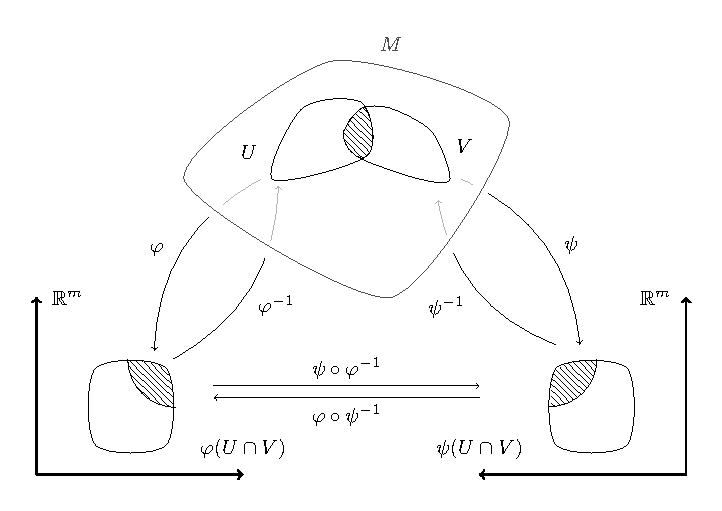
\includegraphics{fig/ch4-atlas-chart.pdf}
    \caption{坐标卡与相容性}\label{chdm:pic_chart}
\end{figure}


\begin{proposition}\label{chdm:thm_biggestDiffStruc}
    设微分流形$M$上有坐标卡集合$\mathscr{B}$满足定义\ref{chdm:def_Dmanifold}中的条件(1)和(2),
    那么在$M$上必然存在唯一的一个微分结构$\mathscr{A}\supset \mathscr{B}$.
\end{proposition}
\begin{proof}
    已知存在坐标卡集合$\mathscr{B}$满足条件(1)和(2),
    索性把所有与$\mathscr{B}$相容的坐标卡都放在一起构造出一个最大的图册,
    称之为$\mathscr{A}$.用这种方式构造的集合$\mathscr{A}$显然满足条件(1)和(2),
    这便是条件(3)中所说的极大图册.
    这种方式构造出的$\mathscr{A}$显然是唯一的.
\end{proof}
这个命题说明:定义\ref{chdm:def_Dmanifold}中的条件(1)和(2)是基本的.


%\subsubsection*{例题}
下面给出几个具体例子.

\begin{example}
    可数离散点集构成的拓扑空间是零维流形.\qed
\end{example}


\begin{example}\label{chdm:exm_trival}
    $m$维欧几里得空间$\mathbb{R}^m$.只需取一个开集$U=\mathbb{R}^m$即可,
    令映射$\varphi:U\to \mathbb{R}^m$是恒等映射,则$(U,\varphi)$是
    空间$\mathbb{R}^m$的坐标卡.
    
    能够与标准欧几里得坐标进行坐标变换的坐标卡有很多,有的变换只连续,并不可微;    
    如果我们将所有变换关系是$C^\infty$可微的坐标卡集合记为$\mathscr{B}$,
    那么$\mathscr{B}$便是$\mathbb{R}^m$的最大图册,也就是它的{\kaishu 微分结构};
    称为$\mathbb{R}^m$的{\kaishu 标准微分结构}. \qed
\end{example}


\begin{example}\label{chdm:exm_bu-tong-jie-gou}
    实数轴$\mathbb{R}$上可以构造不同的微分结构.第一种微分结构取为如例\ref{chdm:exm_trival}所示
    的标准微分结构,记为$\mathscr{A}_1$,局部坐标用$x$表示.
    
    第二种微分结构可以这样构造,取$V=\mathbb{R}$,映射$\psi:V\to \mathbb{R}$取
    为$\psi(y)=y^5, \  \forall y \in V$,记这种结构为$\mathscr{A}_2=(V,\psi)$.
    
    坐标变换$\varphi \circ \psi^{-1}$的表达式为$x=\sqrt[5]{y}$,
    很明显这个函数在$y=0$处不可微,所以两个微分结构并不相容. \qed
\end{example}

\begin{example}\label{chdm:exm_sphere1}
    $\mathbb{R}^{m+1}$中$m$维标准球面$S^m(a)$的微分流形.
\end{example}
$S^m(a)$的具体表示为:
\begin{equation}
    S^m(a)=\left\{(x^1, \cdots, x^{m+1}) \in \mathbb{R}^{m+1} \ | \ \sum_{i=1}^{m+1}(x^i)^2= a^2 \right\} .
\end{equation}
对每一个$\alpha(1\leqslant \alpha \leqslant m+1)$,令
\begin{align*}
    U_\alpha ^{+} &= \{(x^1,\cdots,x^{m+1})\in S^m: x^\alpha > 0 \},  \\
    U_\alpha ^{-} &= \{(x^1,\cdots,x^{m+1})\in S^m: x^\alpha < 0 \}.
\end{align*}
这两个类型的集合是球面$S^m(a)$上的开集,这些集合之并是球面$S^m(a)$的开覆盖,即
\begin{equation}
    S^m(a)= \bigcup_{\alpha=1}^{m+1} \bigl(U_\alpha ^{+} \cup U_\alpha ^{-} \bigr).
\end{equation}
有了开覆盖,下面定义映射$\varphi_\alpha ^{+}: U_\alpha ^{+} \to \mathbb{R}^m$和
$\varphi_\alpha ^{-}: U_\alpha ^{-} \to \mathbb{R}^m$:
\begin{align}
    \varphi_\alpha ^{+}(x^1,\cdots,x^{m+1}) &= (x^1,\cdots,\hat{x}^\alpha, \cdots,x^{m+1}), \\
    \varphi_\alpha ^{-}(x^1,\cdots,x^{m+1}) &= (x^1,\cdots,\hat{x}^\alpha, \cdots,x^{m+1}).
\end{align}
其中$\hat{x}^\alpha$表示把第$\alpha$个分量${x}^\alpha$去掉.
实际上,这两个映射从不同的开集得到了相同的坐标.
在多元微积分角度上看,上面两个映射是$C^\infty$的,它们的逆也是$C^\infty$的;
所以$(U_\alpha ^{+}, \varphi_\alpha ^{+})$和$(U_\alpha ^{-}, \varphi_\alpha ^{-})$是
球面$S^m(a)$的坐标卡.映射$\varphi_\alpha ^{\pm}$(取$\alpha$为固定数值)的几何意义是将$S^m(a)$的
半球面$U_\alpha ^{\pm}$沿第$\alpha$坐标轴投影到$x^\alpha=0$坐标平面上.

下面我们来看坐标变换是否相容.取$\alpha$和$\beta$为两个互不相等的固定数值,
那么必然有$U_\alpha ^{+} \cap U_\beta ^{+} \neq \varnothing$、
$U_\alpha ^{+} \cap U_\beta ^{-} \neq \varnothing$和
$U_\alpha ^{-} \cap U_\beta ^{-} \neq \varnothing$,
我们以$U_\alpha ^{+} \cap U_\beta ^{-}$为例,
写出如下坐标变换的具体公式(见式\eqref{chdm:eqn_sph1f}):
\begin{align*}
    \varphi^-_\beta \circ (\varphi^+_\alpha)^{-1}:& \quad \varphi^+_\alpha
      \bigl( U_\alpha ^{+} \cap U_\beta ^{-} \bigr) \to 
      \varphi^-_\beta \bigl( U_\alpha ^{+} \cap U_\beta ^{-} \bigr),  \\
    \varphi^+_\alpha \circ (\varphi^-_\beta)^{-1}:& \quad \varphi^-_\beta
      \bigl( U_\alpha ^{+} \cap U_\beta ^{-} \bigr) \to 
      \varphi^+_\alpha \bigl( U_\alpha ^{+} \cap U_\beta ^{-} \bigr) .
\end{align*}
其余坐标变换公式留给读者当作练习.
假设$\alpha < \beta$,对于$S^m$球面上的
点$(x^1,\cdots,x^{m+1})\in U_\alpha ^{+} \cap U_\beta ^{-}$有
$x^\alpha >0, \ x^\beta <0$,应用条件$|x|=a$可得坐标变换公式:
\begin{subequations}\label{chdm:eqn_sph1f}
\begin{align}
     &\varphi^-_\beta \circ (\varphi^+_\alpha)^{-1} (x^1,\cdots,\hat{x}^\alpha,\cdots,x^{m+1}) \notag \\
    =&\left(x^1,\cdots,x^{\alpha-1},\sqrt{a^2-\sum\nolimits_{ \gamma\neq \alpha}(x^\gamma)^2},
      x^{\alpha+1},\cdots,\hat{x}^\beta,\cdots,\hat{x}^{m+1}\right), \\
     &\varphi^+_\alpha \circ (\varphi^-_\beta)^{-1} (x^1,\cdots,\hat{x}^\beta,\cdots,x^{m+1}) \notag \\
    =&\left(x^1,\cdots,\hat{x}^\alpha,\cdots, x^{\beta-1},-\sqrt{a^2-\sum\nolimits_{\gamma\neq \beta}(x^\gamma)^2},
      x^{\beta+1},\cdots,\hat{x}^{m+1}\right) .
\end{align}
\end{subequations}
因为式子$\sqrt{a^2-\sum\nolimits_{ \gamma\neq \alpha}(x^\gamma)^2}$和
$\sqrt{a^2-\sum\nolimits_{\gamma\neq \beta}(x^\gamma)^2}$根号下是恒大于零的,
求导之后放在分母上不会导致无穷大,所以两个
坐标变换$\varphi^-_\beta \circ (\varphi^+_\alpha)^{-1}$和
$\varphi^+_\alpha \circ (\varphi^-_\beta)^{-1}$都是$C^\infty$的,
因此坐标卡$(U_\alpha ^{+}, \varphi_\alpha ^{+})$和$(U_\alpha ^{-}, \varphi_\alpha ^{-})$是
$C^\infty$相容的.与此类似同样可证其余坐标卡也是$C^\infty$相容的,所以坐标卡
集合$\{(U_\alpha ^{+}, \varphi_\alpha ^{+}),
(U_\alpha ^{-}, \varphi_\alpha ^{-}): 1\leqslant \alpha \leqslant m+1\}$决定了
球面$S^m(a)$上的$C^\infty$一种微分结构,进而$S^m(a)$符合
定义\ref{chdm:def_Dmanifold}中所有条件,所以它是微分流形.
\qed



\begin{example}\label{chdm:exm_sphere2}
    继上一例题,用球极投影法再次说明$m$维球面是微分流形.
\end{example}
设球面的北极和南极点坐标分别为$N=(0,\cdots,0,a)$和$S=(0,\cdots,0,-a)$.
令$V_{+}=S^m(a)\backslash \{S\},\ V_{-}=S^m(a) \backslash\{N\}$,这样定义的集合是球面上的开集.
分别定义映射$\psi_{\pm}:V_{\pm}\to \mathbb{R}^m$如下
\begin{align}
    (y^1,\cdots,y^m)\equiv &\psi_{+}(x^1,\cdots,x^{m+1}) = 
      \left(\frac{a x^1}{a+x^{m+1}},\cdots, \frac{a x^m}{a+x^{m+1}}\right), 
      \label{chdm:eqn_tmppsip}\\
    (z^1,\cdots,z^m)\equiv &\psi_{-}(x^1,\cdots,x^{m+1}) = 
      \left(\frac{a x^1}{a-x^{m+1}},\cdots, \frac{a x^m}{a-x^{m+1}}\right) .
\end{align}
需要由上两式来求$\psi_{\pm}$的逆映射,我们仅以$\psi_{+}$为例来说明求解过程.
将式\eqref{chdm:eqn_tmppsip}求平方和,并利用$\sum_{i=1}^{m+1}(x^i)^2=a^2$,可得
\begin{align*}
    & \sum_{j=1}^{m}(y^j)^2=\frac{a^2 }{(a+x^{m+1})^2}\left(\sum_{i=1}^{m}(x^i)^2\right)
      =\frac{a^2 }{(a+x^{m+1})^2}\left(a^2-(x^{m+1})^2\right) \\
      {\color{red} \Rightarrow} 
    & x^{m+1} = \frac{a\left(a^2-\sum\nolimits_j(y^j)^2\right)}{a^2+\sum\nolimits_j(y^j)^2},
    {\quad \text{或} \quad } x^{m+1}= -a \ (\text{舍弃}) .
\end{align*}
有了最后一个坐标的表达式,其它坐标几乎一望而知,它们是(同时给出$\psi_{-}^{-1}$)
\begin{align}
    (x^1,&\cdots,x^m, x^{m+1}) = \psi_{+}^{-1}(y^1,\cdots,y^m) \notag \\
      &=\frac{a}{a^2+\sum\nolimits_j(y^j)^2} 
        \left(2 a y^1, \cdots, 2 a y^m,\ a^2-\sum_{j=1}^m(y^j)^2\right), 
        \label{chdm:eqn_sp2yx} \\
    (x^1,&\cdots,x^m, x^{m+1}) = \psi_{-}^{-1}(z^1,\cdots,z^m) \notag \\
      &=\frac{a}{a^2+\sum\nolimits_j(z^j)^2} 
        \left(2 a z^1, \cdots, 2 a z^m,\ \sum_{j=1}^m (z^j)^2 - a^2 \right).
        \label{chdm:eqn_sp2zx}
\end{align}
有了逆映射,便可以求出坐标变换如下
\begin{align}
    (z^1,\cdots,z^m)=& \psi_{-}\circ \psi_{+}^{-1} (y^1,\cdots,y^m)
      = \frac{a^2}{\sum\nolimits_j(y^j)^2}  \left(y^1,\cdots, y^m \right) , \label{chdm:eqn_sp2yz}\\
    (y^1,\cdots,y^m)=& \psi_{+}\circ \psi_{-}^{-1} (z^1,\cdots,z^m) 
      = \frac{a^2}{\sum\nolimits_j(z^j)^2}  \left(z^1,\cdots, z^m \right) . \label{chdm:eqn_sp2zy}
\end{align}
不难验证这些坐标变换都是$C^\infty$的,故$(V_+,\psi_+;y^i)$和$(V_-,\psi_-;z^i)$构成了
球面$S^m(a)$的容许局部坐标开覆盖,决定了球面的一种微分结构.
\qed



\begin{example}\label{chdm:exm_sphere12}
    以$S^1(1)$为例来说明上面两个例题中的坐标卡属于同一微分结构.
\end{example}
只取其中一个坐标变换,其余类似.
取第一种坐标卡中的开集和映射为
\begin{equation*}
    U_1 ^{+} = \{(x^1,x^2)\in S^1: x^1 > 0 \}, \ 
    \varphi_1 ^{+}(x^1,x^2) = x^2, \ 
    (\varphi_1 ^{+})^{-1}(x^2)=\left(\sqrt{1-(x^2)^2},x^2\right) .
\end{equation*}
取第二种坐标卡中的开集和映射为
\begin{equation*}
    V_+, \quad \psi_{+}(x^1,x^2) = \frac{x^1}{1+x^{2}}, \quad
    \psi_{+}^{-1}(y^1) = \frac{1}{1+(y^1)^2}\left(2  y^1, 1-(y^1)^2\right) .
\end{equation*}
坐标变换为
\begin{align}
    \varphi_1 ^{+} \circ \psi_{+}^{-1}(\xi) = \frac{1-\xi^2}{1+\xi^2}, \qquad
    \psi_{+}\circ (\varphi_1 ^{+})^{-1}(\eta) =\frac{\sqrt{1-\eta^2}}{1+\eta} .
\end{align}
这些函数是$C^\infty$的,所以坐标变换是相容的,它们属于同一微分结构.
\qed

{ %\kaishu 
    可见在构造微分流形时,只需指出它的一个相容的坐标覆盖就行了,
    这样已能研究全部的几何.  比如对于球面$S^m(a)$,(对于物理中的应用而言)
    我们用例\ref{chdm:exm_sphere1}或例\ref{chdm:exm_sphere2}中
    的任意一个坐标覆盖即可,(除了微分拓扑等基础领域)
    没有必要非将其延拓至最大相容的坐标覆盖(即微分结构);
    命题\ref{chdm:thm_biggestDiffStruc}表明任意一个坐标覆盖都能延拓至最大图册.}

\subsection{笛卡尔积流形}\label{chdm:sec_cartensian-product}
拓扑空间有笛卡尔积的概念(见定义\ref{chtop:def_cartensian}),微分流形也有类似概念.
%\begin{definition}\label{chdm:def_cartensian-product}
%\end{definition}
设有微分流形$M$和$N$,其维数分别是$m$和$n$,它们的微分结构分别是
\begin{equation}
    \mathscr{A}_1=\{(U_\alpha, \varphi_\alpha)|\alpha\in \mathscr{I}_1 \}, \qquad
    \mathscr{A}_2=\{(V_i, \psi_i)|i\in \mathscr{I}_2 \} .
\end{equation}

由命题\ref{chtop:thm_hcb}、\ref{chtop:thm_cph}可知$M\times N$是Hausdorff空间,并有可数拓扑基;
且$\{(U_\alpha\times V_i)\mid \alpha\in \mathscr{I}_1,i\in \mathscr{I}_2\} $是
拓扑积$M\times N$的一个开覆盖.下面构造$M\times N$的微分结构.
对每一对指标$\{(\alpha,i)\in \mathscr{I}_1 \times \mathscr{I}_2\}$,定义
从$U_\alpha\times V_i$到$\mathbb{R}^{m+n}$的映射如下
\begin{align*}
    (\varphi_\alpha \times \psi_i)(x,y)\overset{def}{=}&\bigl(\varphi_\alpha(x),\ \psi_i(y)\bigr),
    \qquad \forall (x,y)\in U_\alpha\times V_i . \\
    (\varphi_\alpha \times \psi_i)^{-1}(X,Y)\overset{def}{=}&\bigl(\varphi_\alpha^{-1}(X),\ 
    \psi_i^{-1}(Y)\bigr),  \qquad \forall (X,Y)\in \varphi_\alpha(U_\alpha)\times \psi_i(V_i) .
\end{align*}
不难验证$\varphi_\alpha \times \psi_i$是从$U_\alpha\times V_i$
到$\varphi_\alpha(U_\alpha)\times \psi_i(V_i)$的同胚映射.

\index[physwords]{笛卡尔积!微分流形}

再者,当$U_\alpha \cap U_\beta \neq \varnothing,\ V_i\cap V_j\neq \varnothing$时,定义
\begin{equation}
    (\varphi_\alpha \times \psi_i)\circ (\varphi_\beta \times \psi_j)^{-1}
    \overset{def}{=}(\varphi_\alpha\circ \varphi_\beta^{-1})\times
    (\psi_i\circ\psi_j^{-1}) .
\end{equation}
在这样定义下,$(U_\alpha\times V_i , \varphi_\alpha \times \psi_i)$与
$(U_\beta\times V_j , \varphi_\beta \times \psi_j)$是$C^\infty$相容的.
当$U_\alpha \cap U_\beta = \varnothing$和$V_i\cap V_j = \varnothing$至少
有一个成立时,我们约定它们也是$C^\infty$相容的.这样,
\begin{equation}
    \{(U_\alpha\times V_i , \varphi_\alpha \times \psi_i) \mid
    \alpha\in \mathscr{I}_1,i\in \mathscr{I}_2\} ,
\end{equation}
在拓扑积$M\times N$上决定了一个$m+n$维的光滑结构,这使得$M\times N$成
为$m+n$维光滑流形,称为$M$和$N$的笛卡尔{\heiti 积流形}.



很明显,上述流程可以推广到任意有限个流形($M_1,M_2,\cdots$)之积.



\subsection{小结}\label{chdm:sec_tmpdmcon}
微分流形定义要求每个局部开集$U$均同胚于$\mathbb{R}^m$中的开集,
所以流形自然存在局部坐标$\{U;x^i\}$,这个坐标是天生存在的,不需要额外定义;
微分几何所有理论都需要构建在这个坐标基础之上.
但是,流形论本身不依赖于某套特别的坐标系.
因此,那种想完全摆脱局部坐标去构建微分几何理论的想法是错误的.

然而,微分几何理论的却是整体性的,
流形论主要目的是研究在局部坐标变换下而保持不变的性质(如切矢量、外微分式、黎曼曲率等等).
微分几何理论不能只对某个特别的坐标系正确,对其它坐标系不正确;
也就是理论本身必须与坐标系选取无关才可以;
坐标本身没有意义,所有基本理论都不能只依赖某特定局部坐标(Christoffel符号是个例外).
那种想用坐标分量语言来描述微分几何的方式貌似已经过时了.



引入坐标系的目的是为了把几何问题代数化,从而能用代数及微积分的方法来研究几何问题.
选择适当的坐标可以大大简化研究难度,大家在书中看到的各种坐标,
是前人经过长期研究而作出的选择,基本上是最优的了.


举例说明坐标本身没有意义(以下两例中的度量是欧式度量).
\begin{example}
    张三沿直线向东走了一段距离,我们把他走路的起点算作坐标$a$,
    终点坐标记为$b$;但是坐标本身(不论是$a$还是$b$)都没有意义,
    有意义的是由“$b-a$”表示的这段距离;而且这段距离是不随坐标系变换而改变的,
    比如随便将坐标系平移和旋转,这段距离是不变的,但两点坐标的数值却改变了.
\end{example}

\begin{example}\label{chdm:exam_tuoyuan}
    在$\mathbb{R}^3$中的$x-y$平面上,画一个椭圆(称为旧的),中心在原点,长半轴沿$x$,短半轴沿$y$;
    这是最常用的坐标表示形式.我们将坐标轴进行任意旋转(甚至反射),
    那么(新)椭圆可能处于$\mathbb{R}^3$中任意一个平面上,不在$x-y$平面上;
    此时“旧”、“新”椭圆上的坐标几乎不可能一致了,但是椭圆的长、短半轴长度,
    偏心率等等几何量是不变的.这个例子生动地说明了“坐标本身没有意义”,
    我们应该研究那些坐标变换下的不变量.
    
    在牛顿力学中,地球绕太阳旋转,我们依据牛顿第二定律和万有引力公式列出方程,
    如果按照上述“旧”方式取坐标,则方程很容易求解;
    如果按照上述“新”方式取坐标,则方程很难求解,可能需要用数值解法.不论哪个坐标系,
    求得的解必然是同一个椭圆,但地球在“旧”、“新”坐标系中的坐标是不同的.
    可见,即使在经典力学中,研究的仍是坐标变换下的不变量,坐标本身没有意义!
\end{example}



\begin{exercise}
	以$S^2(1)$为例再次论证例题\ref{chdm:exm_sphere12}.
\end{exercise}

\begin{exercise}
	证明例题\ref{chcdg:exm_torus}中的圆环面是$\mathbb{R}^3$中的光滑流形.
\end{exercise}

\begin{exercise}
	证明$x-y$平面可看成由$x$、$y$轴构成的笛卡尔积流形.
\end{exercise}


\begin{exercise}
	设$S^1$是一维单位圆周.证明例题\ref{chcdg:exm_torus}中的圆环面
	可以看成两个圆周的笛卡尔积流形,即$S^1\times S^1$.
\end{exercise}


\section{流形的映射}\label{chdm:sec_map-dm}
读者应该学习过多元微积分中$\mathbb{R}^m$与$\mathbb{R}^n$间映射(或函数)的概念,
那里的内容大都可以推广到流形之间.
\begin{definition}\label{chdm:def_fmapMN}
    设$M$和$N$分别是$m$和$n$维$C^\infty$微分流形,
    存在连续映射$f:M\to N$.{\footnote{读者应能注意到:
            只到这里的$f$只是拓扑流形间的映射,只能谈及连续性,
            无法涉及可微性.}}
    $\forall p\in M$,存在包含$p$的坐标卡$(U,\varphi;x)$以及$N$上
    包含点$q\equiv f(p)$的坐标卡$(V,\psi;y)$,那么可以构造如下映射$\hat{f}$:
    \begin{equation*}
        \hat{f}\equiv \psi \circ f \circ \varphi^{-1} :
        \varphi(U) \bigl(\subset \mathbb{R}^m\bigr) \ \to \ 
        \psi(V) \bigl(\subset \mathbb{R}^n\bigr) .
    \end{equation*}
    如果$\hat{f}$是$C^r$的(即可微到$r(>0)$阶),{\footnote{$\hat{f}$肯定是连续的;
            $\hat{f}$本质上是$\mathbb{R}^m$与$\mathbb{R}^n$开子集间的映射,
            自然可以谈及其可微性.}}
    那么称映射$f:M\to N$在$p$点是$C^r$的;如果$f$在每一点都是$C^r$的,那么称
    之为$C^r$映射.
\end{definition}

\index[physwords]{微分流形!流形间映射}

\begin{remark}\label{chdm:rek_jacobi}
    不难验证,上述定义与坐标卡选取无关.
    有了这个定义后,我们不再严格区分$f$和$\hat{f}$,认为两者等同.
    在多元微积分中$\hat{f}$在$p\in \mathbb{R}^m$点的Jacobi矩阵也称为
    $f$在$p\in M$点的Jacobi矩阵.Jacobi矩阵秩也可作类似认同.
\end{remark}
\begin{definition}\label{chdm:def_fmapCurve}
    设定义\ref{chdm:def_fmapMN}中的$M$是实数轴上的某个开区间$(a,b)$,那么
    称映射$f:(a,b)\to N$为流形$N$上的一条$C^r${\heiti (参数)曲线}. \index[physwords]{微分流形!参数曲线}
\end{definition}
设流形$N$中有$C^r$曲线$f(t)$,其中$t$称为曲线的{\heiti 参数}.如果有$C^r$变换函数$u(t)$将
参数$t$变成$u$,并且$\frac{{\rm d} u }{{\rm d} t}$处处不为零,那么称
变换后的曲线$\tilde{f}(u)=f\bigl(u(t)\bigr)$是原曲线$f(t)$的{\heiti 重参数化曲线}.
既然$\frac{{\rm d} u }{{\rm d} t}$处处不为零,那么必然
有$\frac{{\rm d} u }{{\rm d} t}>0$或者$\frac{{\rm d} u }{{\rm d} t}<0$处处成立,
即变换$u(t)$是单调的双射函数.

\begin{definition}\label{chdm:def_func}
    设定义\ref{chdm:def_fmapMN}中的$N$是实数轴上的某个开区间$(a,b)$,那么
    称映射$f:M \to (a,b)$为流形$M$上的$C^r${\heiti 函数}.
    全体$C^r$函数集合记作$C^r(M)$.
\end{definition}
函数的加法和乘法在$C^r(M)$中是封闭的,(参照\pageref{chtop:def_ring}页
定义\ref{chtop:def_ring})因此$C^r(M)$在代数上是一个{\kaishu 环}.

\index[physwords]{微分流形!函数}

\begin{example}
    设流形$M$的局部坐标是$(U_\alpha,\varphi_\alpha;x^i)$,在局部坐标系下
    有$\frac{\partial x^i}{\partial x^j}=\delta^i_j$,这明确说明:
    当把局部坐标$x^i$看成函数时,它一定是$C^\infty$的.
\end{example}

\begin{definition}\label{chdm:def_Diff-Homeomorphism}
    设定义\ref{chdm:def_fmapMN}中的$f$是拓扑同胚(见\ref{chtop:def_homeomorphism}),
    若$f$和$f^{-1}$都是$C^r$的,则称$f$是微分流形$M$与$N$间的$C^r${\heiti 微分同胚}.
    若$f$只是$M$的某局部开集$U$和$N$的局部开集$V$之间的微分同胚,
    则称$f$为$U$到$V$上的{\heiti 局部微分同胚}.
\end{definition}
拓扑同胚可保证两流形维数相等(见定义\ref{chtop:def_topological-manifold}后讨论);
微分同胚自然也可得此结论.

\index[physwords]{微分流形!微分同胚、光滑同胚}

下面叙述几个关于映射的命题,这些命题会在多处使用.
为理解方便,先介绍$\mathbb{R}^m$空间中的一个命题:
\begin{proposition}\label{chdm:thm_exp1Rm}
    令$Q$是$\mathbb{R}^m$中的一个矩形区域.存在一个$C^\infty$函
    数$\phi:\mathbb{R}^m \to \mathbb{R}$使得当$x$属于$Q$内部时,
    有:$\phi(x)>0$;否则$\phi(x)=0$.
\end{proposition}
\begin{proof}
    先考虑如下一维函数$f:\mathbb{R} \to \mathbb{R}$,
    \begin{equation*}
        f(t)=\begin{cases}
            \exp(-\tfrac{1}{t}), & t > 0 ;\\
            0, & t \leqslant 0 .
        \end{cases}
    \end{equation*}
    此函数曲线见图\ref{chdm:pic_exp1},当$t\to \infty$时,$f(t)\to 1^-$;
    当$t\to 0^+$时,$f(t)\to 0$;拐点在$t=0.5$处.
    很明显,函数$f$在实数轴上是$C^\infty$的.利用此函数,接着
    定义另一函数$g$(见图\ref{chdm:pic_exp2}),
    \begin{equation}\label{chdm:eqn_g1}
        g(t)=f(t)\cdot f(1-t)/(f(0.5))^2 .
    \end{equation}
    函数$g$在$0<t<1$中非零且恒正,其它点恒为零;最大值已归一化到$1$.
    
    对于高维空间$\mathbb{R}^m$中的矩形
    区域$Q=[a_1,b_1]\times \cdots \times[a_m,b_m]$,
    则可定义函数$\phi$如下
    \begin{equation}\label{chdm:eqn_gexpphi1}
        \phi(x)=g\left(\frac{x_1 -a_1}{b_1-a_1}\right) \times 
        g\left(\frac{x_2 -a_2}{b_2-a_2}\right) \times \cdots \times
        g\left(\frac{x_m -a_m}{b_m-a_m}\right) .
    \end{equation}
    这样定义的函数满足命题要求,这便证明了存在性.
    需要指出的是这类函数有很多,不止上述一个.
\end{proof}


\begin{figure}[htb]
    \begin{minipage}[t]{0.5\linewidth}
        \centering
        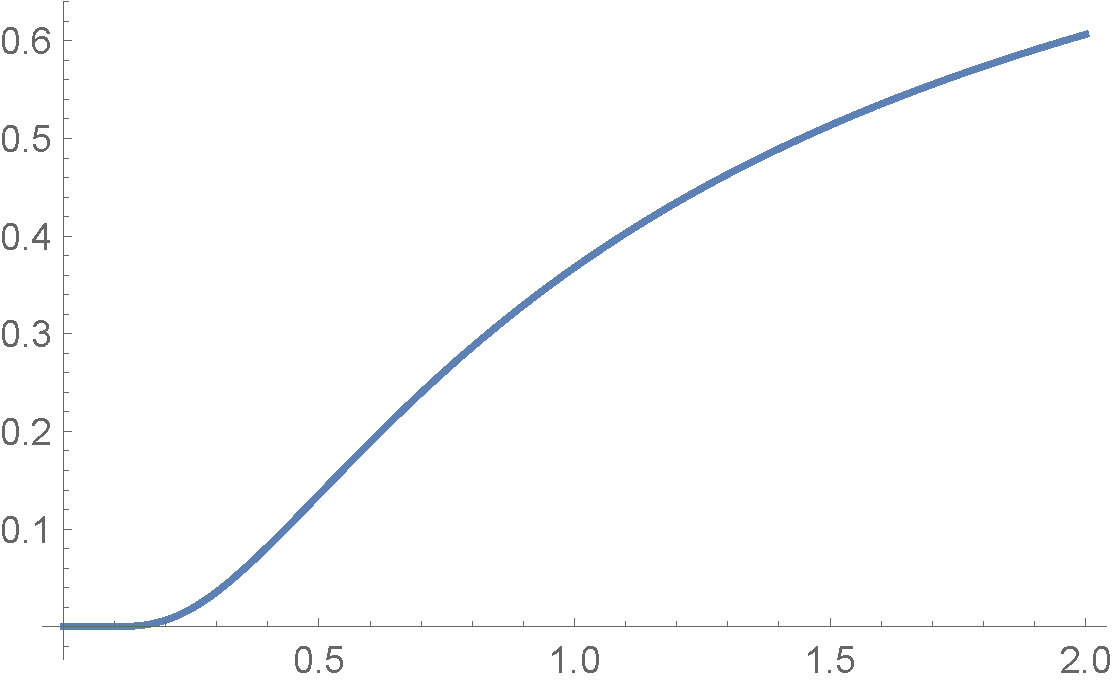
\includegraphics[scale=0.3]{fig/ch4-exp1.pdf}
        \caption{指数函数$f$}\label{chdm:pic_exp1}
    \end{minipage}%
    \begin{minipage}[t]{0.5\linewidth}
        \centering
        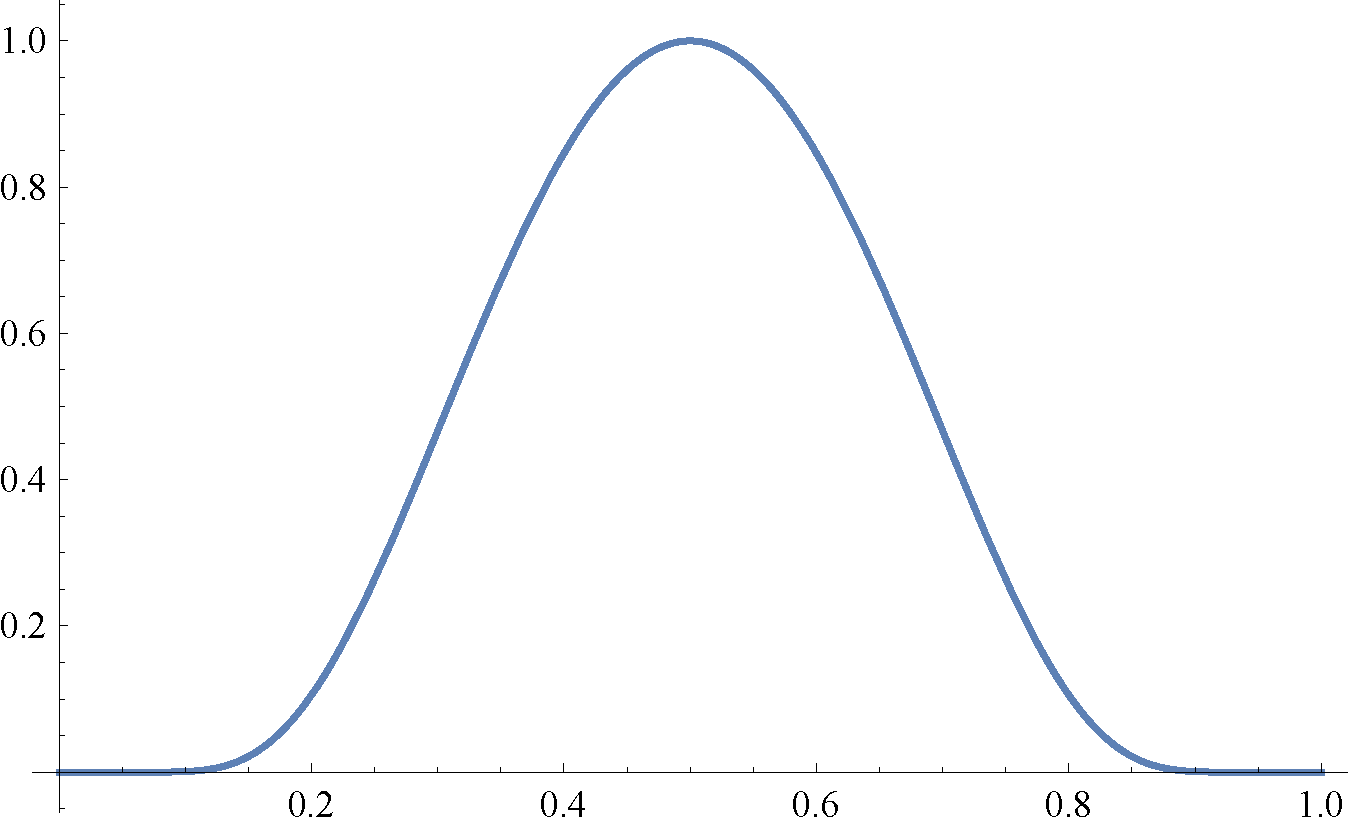
\includegraphics[scale=0.3]{fig/ch4-exp2.pdf}
        \caption{指数函数积$g$}\label{chdm:pic_exp2}
    \end{minipage}
\end{figure}

上面命题还有变种.
\begin{proposition}\label{chdm:thm_exp1RmSphere}
    令$D_1$和$D_2$是$\mathbb{R}^m$中两个同心球,且$\overline{D}_1 \subset D_2$.
    则存在$C^\infty$函数$f:\mathbb{R}^m \to \mathbb{R}$使
    得$0\leqslant f \leqslant 1$,并且
    \begin{equation}\label{chdm:eqn_exp1RmSphere}
        f(x)=\begin{cases}
            1, & x\in D_1 ; \\
            0, & x\notin D_2 .
        \end{cases}
    \end{equation}
\end{proposition}
上面命题将取值域限定为球,这个限制可以拓展至一般情形:
\begin{proposition}\label{chdm:thm_exp1UVRm}
    令$U$和$V$是$\mathbb{R}^m$中两个非空开集,$\overline{V}$是紧致的,
    且$\overline{V} \subset U$.
    则存在$C^\infty$函数$g:\mathbb{R}^m \to \mathbb{R}$使
    得$0\leqslant g \leqslant 1$,并且
    \begin{equation}\label{chdm:eqn_exp1UVRm}
        g(x)=\begin{cases}
            1, & x\in V ; \\
            0, & x\notin U .
        \end{cases}
    \end{equation}
\end{proposition}
上面命题可以推广到一般流形上:
\begin{proposition}\label{chdm:thm_exp1UVM}
    令$U$和$V$是微分流形$M$中两个非空开集,$\overline{V}$是紧致的,
    且$\overline{V} \subset U$.
    则存在$C^\infty$函数$h:M \to \mathbb{R}$使
    得$0\leqslant h \leqslant 1$,并且
    \begin{equation}\label{chdm:eqn_exp1UVM}
        h(p)=\begin{cases}
            1, & p\in V ; \\
            0, & p\notin U .
        \end{cases}
    \end{equation}
\end{proposition}
命题\ref{chdm:thm_exp1RmSphere}、
\ref{chdm:thm_exp1UVRm}和\ref{chdm:thm_exp1UVM}的证明
并不复杂,可参见文献\parencite[\S 1.3]{cc2001-zh}中证明.
它们本质上是命题\ref{chdm:thm_exp1Rm}的推广,但越来越抽象.
利用命题\ref{chdm:thm_exp1UVM},可证明下面命题:
\begin{proposition}\label{chdm:thm_Flocal-equiv-Fglobal}
    设$U$是微分流形$M$的一个开子集,给定函数$f\in C^\infty(U)$,
    则$\forall p\in U$,必有$p$点一个邻域$V\subset U$,以及光滑
    函数$\hat{f}\in C^\infty(M)$,使得$\hat{f}|_V = f|_V$.
\end{proposition}
\begin{proof}
    利用流形的局部紧致性,可以使得$\overline{V}$是$U$的真子集;如果不是,
    将$V$缩小一些即可.依照命题\ref{chdm:thm_exp1UVM},存在
    流形$M$上的光滑函数$h$满足式\eqref{chdm:eqn_exp1UVM},令
    \begin{equation}
        \hat{f}(x)=\begin{cases}
            f(x)\cdot h(x), & \forall x\in V ; \\
            0, & \forall x\notin U .
        \end{cases}
    \end{equation}
    很明显,有$\hat{f}|_V = f|_V$.因$f$在$U$上式光滑的,故$f\cdot h$在$V$上也是
    光滑的;而$h$又保证了$\hat{f}$能以$C^\infty$的方式光滑从$V$过渡到$M\backslash U$,
    所以$\hat{f}$是整个流形$M$上的光滑函数.
\end{proof}
这个命题是说:局部的光滑函数可以很容易地延拓成整个流形上的光滑函数.
反之,光滑流形$M$上的光滑函数场也可以限制在开子集$V$上.


\begin{exercise}
	证明本节未给出证明过程的定理(命题).
\end{exercise}

\section{切空间}\label{chdm:sec_tangentspace}
在\S\ref{chdm:sec_ed}中,我们给出了欧氏空间切矢量的定义\ref{chdm:def_tang-vec-inEV};
现在有了微分流形概念,
可以把定义\ref{chdm:def_tang-vec-inEV}移植到流形论中.
本节先定义切矢量,再引入余切矢量.这个过程也可以反过来,
即先定义余切矢量,再引入切矢量;可参考\parencite[\S 1.2]{cc2001-zh}.

\index[physwords]{切空间}

\subsection{切矢量}
\begin{definition}\label{chdm:def_tang-vec-inManifold}
    设有一$m$维$C^\infty$微分流形$M$,任选其中一点$x\in M$.
    点$x$上{\heiti 切矢量}(简称{\heiti 矢量})$v^a$是指
    满足如下条件的一个映射$v^a:C_x^\infty(M)\to \mathbb{R}$  \index[physwords]{切矢量}
        
    {\bfseries (1)} 线性性:$\forall g,h \in C^\infty_x(M) $ , $\forall \lambda \in \mathbb{R}$,有
    $v (g+\lambda h) = v (g)+ \lambda v (h) ;$
    
    {\bfseries (2)} Leibnitz律:$\forall g,h \in C^\infty_x(M) $,有
    $v (g\cdot h) = \bigl(v(g)\bigr)\cdot h(x)+ g(x)\cdot v (h) .$
\end{definition}

在\S\ref{chdm:sec_ed}中,我们将方向导数等同于切矢量,这个认知在流形中也是成立的.
设映射$\gamma:(-a,a)\to M$是微分流形$M$中一条经过固定点$x_0$的光滑曲线,
其中$x_0=\gamma(0)$,则下面的映射$v^a:C^\infty_{x_0}\to \mathbb{R}$(其中$f\in C_{x_0}^\infty(M)$)
\begin{equation}\label{chdm:eqn_DiffCurve}
    v(f)\overset{def}{=} \left. \frac{{\rm d} \bigl(f \circ \gamma (t)\bigr)}{{\rm d} t} \right |_{t=0}
    \equiv \left. \frac{{\rm d} \Bigl(f \bigl(\gamma (t)\bigr)\Bigr)}{{\rm d} t} \right |_{t=0};
    \quad -a < t < a, \quad a>0.
\end{equation}
便确定了$x_0$点的一个切矢量$v^a$;只需验证上面公式满足定义即可.
线性性的验证是一望而知的.下面验证Leibnitz律;需要先指出
\begin{equation}\label{chdm:eqn_f-cdot-g-circo-gamma}
    (f\cdot g)\circ \gamma \overset{def}{=} (f\circ \gamma) \cdot (g\circ \gamma)  .
\end{equation}
将上式带入式\eqref{chdm:eqn_DiffCurve},有
\begin{align*}
    v(f\cdot g)=& \left. \frac{{\rm d} \Bigl(f \bigl(\gamma (t)\bigr)\cdot 
        g \bigl(\gamma (t)\bigr)\Bigr)}{{\rm d} t} \right |_{t=0} \\
    =& \left. \frac{{\rm d} \Bigl(f \bigl(\gamma (t)\bigr)
        \Bigr)}{{\rm d} t} \right |_{t=0} \cdot g \bigl(\gamma (0)\bigr) +
      f \bigl(\gamma (0)\bigr)\cdot \left. \frac{{\rm d} \Bigl( 
        g \bigl(\gamma (t)\bigr)\Bigr)}{{\rm d} t} \right |_{t=0} \\
    =& \bigl(v(f)\bigr)\cdot g(x_0)+ f(x_0)\cdot v (g) .
\end{align*}
验证完毕.
公式\eqref{chdm:eqn_DiffCurve}中所定义的切向量称为曲线$\gamma(t)$在$t=0$的{\heiti 切矢量}.
%当取遍$x_0$的所有曲线,全部这些切矢量会构成一个线性空间.
这个例子非常生动地说明了切矢量和方向导数是一回事儿!

\begin{remark}\label{chdm_rek-vnoa}
    $v(f)$是一个实数,如果写成$v^a(f)$可能
    会被误认为是一个矢量,所以略去抽象指标.
    后面切矢量\uwave{场}作用在标量函数场上时也不采用抽象指标记号.
\end{remark}
局部坐标本身就是一个$\mathbb{R}^m$,具有线性结构,我们选取
这样的曲线$\gamma_j:(-a_j,a_j)\to M,\ 1\leqslant j \leqslant m$使得其局部坐标是
\begin{equation}\label{chdm:eqn_gammaj}
    x^i\bigl({\gamma_j}(t)\bigr)= x^i_0 + \delta^i _j \cdot t,
\end{equation}
上式中指标$j$是固定不变的,上标$i$是其$m$个坐标分量的指标.
当$i\neq j$时,坐标就处在$x^i_0$点不动;
当$i=j$时,(只有这一个)坐标按线性规律(即直线)变化.
将这样的坐标带入式\eqref{chdm:eqn_DiffCurve},并将这个切矢量
记为$(\frac{\partial }{\partial x^j})^a$(注意作用到标量函数上后,略去抽象指标)
\begin{align*}
    \frac{\partial }{\partial x^j} f\bigl(\gamma (0)\bigr) =& \left. 
    \frac{{\rm d} (f \circ\varphi^{-1}) \circ\bigl(\varphi\circ \gamma (t)\bigr)}{{\rm d} t}  \right |_{t=0}
    =  \left. \frac{{\rm d} (f \circ\varphi^{-1}) (x^1_0,\cdots, x^j_0 + t, \cdots ,x^m_0)}{{\rm d} t}  \right |_{t=0}  \\
    =& \left.\frac{\partial (f \circ\varphi^{-1})}{\partial x^j}\right|_{\varphi(x_0)} 
    \left.\frac{{\rm d}(x^j_0 + t) }{{\rm d} t} \right|_{t=0}
    = \left.\frac{\partial (f \circ\varphi^{-1})}{\partial x^j}\right|_{\varphi(x_0)} .
\end{align*}
很明显切矢量\eqref{chdm:eqn_DiffCurve}在坐标\eqref{chdm:eqn_gammaj}下就表现为对
标量函数$f$求坐标$x^j$的偏导数,这也是将其记为$(\frac{\partial }{\partial x^j})^a$的理由;
这样的偏导数(也就是切矢量)共有$m$个,即$j=1,\cdots,m$.

\subsection{切空间基矢}
上面定义中已给出切矢量对$C^\infty_x(M)$中全体(标量)函数具有线性性.
若在不同切矢量间定义如下关系:
\begin{subequations}
    \begin{align}
        (u+v)f & \overset{def}{=} u(f) + v(f),\qquad {\text {$u,v$是$x\in M$的任意切矢量}}; \\
        (\lambda u) f & \overset{def}{=} \lambda \bigl( u(f)\bigr), \qquad \forall\lambda\in \mathbb{R}.
    \end{align}
\end{subequations}
上两式中$f\in C^\infty_x(M)$.有了这样定义之后,不难发现$x\in M$点{\kaishu 全体切矢量}满足
线性空间的定义\ref{chmla:def_linear-space},我们称这个线性空间是微分流形$M$在
点$x$的{\heiti 切空间},记为$T_x M$.下面我们证明这个空间的维数恰好是$m$;
大体思路是:首先找到$m$个切矢量,然后证明它们线性无关,最后证明每个切矢量都可以由它们展开.

\index[physwords]{切空间!基矢}

设微分流形$M$在点$x_0$的邻域的容许坐标卡是$(U,\varphi;x)$,点$x_0$的坐标
是$(x^1_0,\cdots,x^m_0)$.%式\eqref{chdm:eqn_DiffCurve}已经给出一个切矢量的定义,仿照它,不难验证(留给读者当练习)
前面已经指出了
\begin{equation}
    \left. \left(\frac{\partial }{\partial x^i}\right)^a \right|_{x_0}, \qquad 1\leqslant i \leqslant m,
\end{equation}
是点$x_{0}\in U$的切矢量.需注意:局部开子集$U$与$\mathbb{R}^m$是拓扑同胚的,天生有坐标,
天生有偏导数的概念,无需另行定义;或者直接将$U$与$\mathbb{R}^m$作恒等认同.

用反证法.假设存在$m$个不全为零的实常数$c^i$使得下式成立:
\begin{equation}
    c^i \frac{\partial f}{\partial x^i}  =0, \qquad \forall f \in C^\infty(U).
\end{equation}
将标量函数$f$选为坐标线$x^k$,并将这些坐标线一一带入上式,
容易得到$c^k=0,\ k=1,\cdots,m$.与假设矛盾,所以$m$个矢量是线性无关的.

任意给定一个满足定义\ref{chdm:def_tang-vec-inManifold}的矢量$v^a\in T_{x_0}M$,
下面证明它可以由$(\frac{\partial }{\partial x^j})^a$展开.证明过程
与定理\ref{chdm:thm_tang-vec-inEV}证明非常相似.
仿照命题\ref{chdm:thm_dc0}证明可以得到:满足
定义\ref{chdm:def_tang-vec-inManifold}的矢量$v^a$作用到任意
实常数$c$上都使之为零,即$v(c)\equiv 0$.

同样,由多元函数微分中值定理可知,$\forall f\in C_{x_0}^\infty(M)$,有
\setlength{\mathindent}{0 em}
\begin{equation*} %\label{chdm:eqn_wfzzdlM}
    (f \circ\varphi^{-1})(x^1,\cdots,x^m)=(f \circ\varphi^{-1})(x^1_0,\cdots,x^m_0)+ 
    (x^i-x^i_0) \frac{\partial (f \circ\varphi^{-1}) \bigl(x_0+\theta(x-x_0) \bigr)}{\partial x^i},
\end{equation*}\setlength{\mathindent}{2 em}
其中$0<\theta<1$.将矢量$v^a$作用到上式,可得(请参考定理\ref{chdm:thm_tang-vec-inEV}证明)
\begin{align*} %\label{chdm:eqn_wfzzdlM}
    v\bigl( f \circ\varphi^{-1} (x^1,\cdots,x^m)\bigr) = v(x^i-x^i_0) \cdot      \left.
     \frac{\partial (f \circ\varphi^{-1}) \bigl(x_0+\theta(x-x_0) \bigr)}{\partial x^i}\right|_{x=x_0}.
\end{align*}
记$v^i\equiv v(x^i)$,并将坐标省略,上式变为(将$f \circ\varphi^{-1}$记为$\hat{f}$)
\begin{equation}\label{chdm:eqn_v-expand-on-natural-bases}
    v( \hat{f} ) = v^i \cdot 
    \frac{\partial \hat{f} (x_0)}{\partial x^i}
    {\quad \color{red}\Leftrightarrow \quad }
    v^a = \sum_{i=1}^{m} { v^i \left(\frac{\partial }{\partial x^i}\right)^a_{x_0} }.
\end{equation}
上面“${ \color{red}\Leftrightarrow }$”后的式子将$\hat{f}\equiv f \circ\varphi^{-1} $略
去(因$f$和$\varphi$都是任选的),并补上了抽象指标记号.
上式充分说明$x_0$点任意矢量$v^a$都可以由$m$个$x_0$点矢量$(\frac{\partial }{\partial x^i})^a_{x_0} $展开,
其系数是$m$个实数$v^i\equiv v(x^i)$.

因此,$\{(\frac{\partial }{\partial x^i})^a_{x_0}, \ 1\leqslant i\leqslant m\}$是线性空间$T_{x_0}M$的
一组基矢量,称之为{\heiti 自然坐标(切)基底},简称自然基底;空间$T_{x_0}M$的维数是$m$.

\index[physwords]{切空间!自然坐标基矢}
\index[physwords]{切矢量!曲线切矢}

\begin{example}\label{chdm:exm_DiffCurve}
    式\eqref{chdm:eqn_DiffCurve}给出了光滑曲线$\gamma(t)$的切矢量,我们用自然基底来表示这个切矢量.
    设$m$维光滑流形$M$有局部坐标系$(U;x^i)$,$\forall p\in U$($p$对应$t=0$),曲线$\gamma(t)$上点的
    局部坐标记为$\{x^i\}$.将式\eqref{chdm:eqn_DiffCurve}展开为
    \setlength{\mathindent}{-0.2 em}
    \begin{equation}\label{chdm:eqn_DiffCurve-2}
        \left. \frac{{\rm d} \bigl(f \circ \gamma (t)\bigr)}{{\rm d} t} \right |_{t=0}
        = \frac{\partial f}{\partial x^i}
        \left. \frac{{\rm d} x^i\circ\gamma (t)}{{\rm d} t} \right |_{t=0}
        {\color{red}\Rightarrow}
        \left. \left(\frac{{\rm d}  }{{\rm d} t}\right)^a \right |_{\gamma (0)}
        = \frac{{\rm d} x^i\bigl(\gamma (0)\bigr)}{{\rm d} t}
        \left(\frac{\partial }{\partial x^i}\right)^a .
    \end{equation}\setlength{\mathindent}{2em}
    上式中“${\color{red}\Rightarrow}$”是因为$f \in C^\infty_p(M)$的任意性.
    这便是曲线$\gamma(t)$在$p$点切矢量的局部坐标展开式;
    其中切矢量$\left(\frac{{\rm d}  }{{\rm d} t}\right)^a $必需沿曲线$\gamma(t)$,
    且取$t=0$.
    
    \index[physwords]{切矢量!切线切矢量} \index[physwords]{切线切矢量}
    
    注:一般称$\left(\frac{{\rm d}  }{{\rm d} t}\right)^a $是
    曲线$\gamma(t)$切线的切矢量,简称{\heiti 切线切矢量}. 
    比如二维球面$S$上任一点$p$的切平面$T$上的任意(原点在切点$p$的)矢量都是切于球面$S$的.
    再取过$p$点的一个大圆$\gamma(t)$,切平面上的切矢量未必切于大圆$\gamma(t)$.
    “切线切矢量”是笔者杜撰出来的名词,
    用来描述切于曲线$\gamma(t)$的切矢量,以区别于切平面$T$上其它切矢量.
\end{example}


\index[physwords]{余切空间}
\index[physwords]{余切矢量}

\subsection{余切空间}
切空间是一个$m$维线性空间,按照\S\ref{chmla:sec_dual}内容,它应该有对偶空间.
\begin{definition}
    切空间$T_{x_0}M$的对偶空间称为微分流形$M$在点$x_0$的{\heiti 余切空间},
    记作$T_{x_0}^{*}M$.余切空间的元素称为{\heiti 余切矢量}.
\end{definition}
\S\ref{chmla:sec_dual}中所有内容都可以移植到余切空间;首先,
余切空间维数与切空间相同,都是$m$维;其次,
利用式\eqref{chmla:eqn_dual-bases}定义自然切基矢的{\heiti 对偶自然基矢},
将其记为$({\rm d}x^j)_a$(由于点${x_0}$的标记位置与对偶基矢抽象指标位置重合,暂将${x_0}$略去):
\begin{equation}\label{chdm:eqn_dual-natural-bases}
    ({\rm d}x^j)_a \left(\frac{\partial }{\partial x^i}\right)^a_{x_0} \equiv 
    \left< ({\rm d}x^j)_a , \   \left(\frac{\partial }{\partial x^i}\right)^a_{x_0}\right>
    \overset{def}{=} \delta^j_i .
\end{equation}
由上式定义的对偶基矢共有$m$个.
将$({\rm d}x^j)_a$作用在任意矢量$v^a$上,有
\begin{equation*}
    ({\rm d}x^j)_a v^a =  ({\rm d}x^j)_a 
       \left[v^i \left(\frac{\partial }{\partial x^i}\right)^a_{x_0}\right] 
    =  v^i \left[ ({\rm d}x^j)_a  \left(\frac{\partial }{\partial x^i}\right)^a_{x_0}\right] 
    =  v^i \delta^j_i = v^j .
\end{equation*}
这说明$({\rm d}x^j)_a$的作用是取出$v^a$在自然坐标基底上的第$j$分量.

任意余切空间元素$\omega_a \in T_{x_0}^{*}M$都可以在自然对偶基矢上展开,
并将其作用到任一切矢量$v^a$上,有
\begin{equation}
    \omega_a (v^a) = \left[\omega_j({\rm d}x^j)_a\right] 
      \left(v^i \left(\frac{\partial }{\partial x^i}\right)^a_{x_0}\right) = 
     \omega_j v^i \delta^j_i = \omega_j v^j .
\end{equation}
上式说明对偶矢量和切矢量的线性映射是一个实数;而切矢量$v^a$作用到标量函数$f$上也得到一个
实数$v(f)$;结合这两点,可说明标量函数$f$可以诱导出一个对偶矢量,记为$({\rm d}f)_a$;具体过程如下:
\begin{equation}\label{chdm:eqn_dfv}
    ({\rm d}f)_a v^a \equiv v(f)  %= v^i \left.\frac{\partial f}{\partial x^j}\right|_{x_0}
    = v^i  \delta_i^j  \left.\frac{\partial f}{\partial x^j}\right|_{x_0}
    = \left[v^i  \left(\frac{\partial }{\partial x^i}\right)^a_{x_0}\right] \left[
      ({\rm d}x^j)_a  \left.\frac{\partial f}{\partial x^j}\right|_{x_0} \right] .
\end{equation}
我们说了$({\rm d}f)_a$是由$f$诱导的对偶矢量,自然令$({\rm d}f)_a v^a$ 等于$v(f)$,也可看成定义.
上式计算过程用到了式\eqref{chdm:eqn_v-expand-on-natural-bases}和
式\eqref{chdm:eqn_dual-natural-bases}.由上式可见,$f$诱导的对偶矢量$({\rm d}f)_a$可以看成
\begin{equation}\label{chdm:eqn_df}
    ({\rm d}f)_a = ({\rm d}x^j)_a \left.\frac{\partial f}{\partial x^j}\right|_{x_0} .
\end{equation}
将此式去掉抽象指标,很明确地显示了由$f$诱导的对偶矢量是其普通{\heiti 微分}${\rm d}f$.
这也是我们将标量函数$f$(包括坐标基矢$x^i$)诱导的对偶矢量记成微分的
理由(也见式\eqref{chdm:eqn_dual-natural-bases}).

对于余切矢量认知,也可以先把式\eqref{chdm:eqn_dfv}当成定义,然后由此
立刻导出坐标基矢间的内积公式\eqref{chdm:eqn_dual-natural-bases};再导出其它公式.
很明显定义\eqref{chdm:eqn_dual-natural-bases}和式\eqref{chdm:eqn_dfv}是相容的.


\begin{remark}
读者需注意:抽象指标作用之一是标记张量类型;当不用于求和哑标时,直接去掉后
就变成了\S\ref{chmla:sec_tensor}记号方式;此时,自然坐标切基矢是
偏导数($(\frac{\partial }{\partial x^i})^a\to \frac{\partial }{\partial x^i}$),
自然坐标对偶基矢是普通微分式($({\rm d}x^j)_a \to {\rm d}x^j$).
\end{remark}

\subsection{局部坐标变换}\label{chdm:sec_coortrans}
微分流形定义中要求坐标卡可以取成各种相容形式,如果$x_0\in M$有两个相互容许的
坐标卡$(U,\varphi;x)$和$(V,\psi;y)$,且$U\cap V \neq \varnothing$;
对应的自然坐标基底分别是$(\frac{\partial }{\partial x^i})^a_{x_0} $
和$(\frac{\partial }{\partial y^j})^a_{x_0} $.
我们把$(\frac{\partial }{\partial y^j})^a_{x_0} $看成
式\eqref{chdm:eqn_v-expand-on-natural-bases}中的$v^a$,那么有
\begin{equation}\label{chdm:eqn_xy-transform}
    \left(\frac{\partial }{\partial y^j}\right)^a_{x_0} = \left. \frac{\partial x^i}{\partial y^j}\right|_{x_0} \cdot
    \left(\frac{\partial }{\partial x^i}\right)^a_{x_0}     {\ \Leftrightarrow \ }
    \left(\frac{\partial }{\partial x^i}\right)^a_{x_0} = \left. \frac{\partial y^j}{\partial x^i}\right|_{x_0} \cdot
    \left(\frac{\partial }{\partial y^j}\right)^a_{x_0} .
\end{equation}
上式同时写出了逆变换;可见过渡矩阵恰好是$x_0$点的Jacobi矩阵.

\index[physwords]{切空间!坐标变换}

在$U\cap V$中可以把$y^j$看成自变量是$x^i$的标量函数(也可反过来),
将式\eqref{chdm:eqn_df}中的$f$用$y^j$替换后,有
\begin{equation}\label{chdm:eqn_xy-cov-transform}
    ({\rm d}y^j)_a = ({\rm d}x^i)_a \left.\frac{\partial y^j}{\partial x^i}\right|_{x_0} 
    {\quad \Leftrightarrow \quad }
    ({\rm d}x^i)_a = ({\rm d}y^j)_a \left.\frac{\partial x^i}{\partial y^j}\right|_{x_0} 
\end{equation}
过渡矩阵恰好是$x_0$点的Jacobi矩阵之逆.

其实,在同一流形$M$中,点$x_0\in M$有两个相互容许的坐标卡$(U,\varphi;x)$和$(V,\psi;y)$,
且$U\cap V \neq \varnothing$;此时的局部坐标变换与局部微分同胚是等价的,
一般分别称它们为被动模式和主动模式.请读者仔细理解这两种操作的等价性.


\subsection{张量}\label{chdm:sec_tensor-p}
有了切空间$T_{x_0}M$及其对偶空间$T_{x_0}^{*}M$(两个都是线性空间),
仿照\S\ref{chmla:sec_tensor},可以定义微分流形$M$在点$x_0$处的$\Tpq{p}{q}$型张量,
可以把它看成$m^{p+q}$维线性空间
\begin{equation}\label{chdm:eqn_TM-TsM}
    \mathcal{T}^p_q(x_0) \equiv \underbrace{T_{x_0}M\otimes \cdots \otimes T_{x_0}M}_{p\text{个}}
    \otimes \underbrace{T_{x_0}^{*}M\otimes \cdots \otimes T_{x_0}^{*}M}_{q\text{个}}
\end{equation}
中的元素.也可以把它看成笛卡尔积空间
\begin{equation}\label{chdm:eqn_TM-X-TsM}
    \underbrace{T_{x_0}^{*}M \times \cdots \times T_{x_0}^{*}M}_{p\text{个}}
    \times \underbrace{T_{x_0}M\times \cdots \times T_{x_0}M}_{q\text{个}}
\end{equation}
的$p+q$重线性函数.

\index[physwords]{切空间!张量}

从上一小节可知线性空间$\mathcal{T}^p_q(x_0)$的自然基矢量是(略去了下标$x_0$)
\begin{equation}\label{chdm:eqn_tensortrans}
    \left(\frac{\partial }{\partial x^{i_1}}\right)^{a_1} \otimes \cdots \otimes
    \left(\frac{\partial }{\partial x^{i_p}}\right)^{a_p} \otimes
    ({\rm d}x^{j_1})_{b_1} \otimes \cdots \otimes ({\rm d}x^{j_q})_{b_q} .
\end{equation}
上式中$1\leqslant \{i,j\} \leqslant m $.
由式\eqref{chdm:eqn_xy-transform}和\eqref{chdm:eqn_xy-cov-transform}不难得到
上式在坐标变化下的变换关系.通常省略张量积符号$\otimes$.

$\mathcal{T}^p_q(x_0)$中的任一张量可以在基矢组\eqref{chdm:eqn_tensortrans}上展开,
\begin{equation}\label{chdm:eqn_tensor-component}
    \alpha^{a_1 \cdots a_p}_{\phantom{a_1 \cdots a_p}b_1\cdots b_q} 
     = \alpha^{i_1 \cdots i_p}_{\phantom{i_1 \cdots i_p}j_1\cdots j_q} 
      \left(\frac{\partial }{\partial x^{i_1}}\right)^{a_1} \cdots 
      \left(\frac{\partial }{\partial x^{i_p}}\right)^{a_p} 
      ({\rm d}x^{j_1})_{b_1} \cdots  ({\rm d}x^{j_q})_{b_q}    .
\end{equation}
当坐标变换时,由式\eqref{chdm:eqn_xy-transform}和\eqref{chdm:eqn_xy-cov-transform}易得
分量的变换关系是
\begin{equation}\label{chdm:eqn_tensor-component-trans}
    \tilde{\alpha}^{k_1 \cdots k_p}_{\phantom{k_1 \cdots k_p}l_1\cdots l_q} (y)
    ={\alpha}^{i_1 \cdots i_p}_{\phantom{i_1 \cdots i_p}j_1\cdots j_q} (x) \times
    \frac{\partial y^{k_1}}{\partial x^{i_1}} \cdots 
    \frac{\partial y^{k_p}}{\partial x^{i_p}} \times
    \frac{\partial x^{j_1}}{\partial y^{l_1}} \cdots 
    \frac{\partial x^{j_q}}{\partial y^{l_q}} .
\end{equation}
需要强调的是:上式所有量都需在点$x_0\in M$取值,
$\{x\}$、$\{y\}$是$x_0$点某个小邻域的两套坐标系.
由此式直接可得一阶切矢量或余切矢量的分量变换关系.


\subsection*{小结}
本小节引入了诸多概念:切矢量、切空间、余切空间、自然坐标切基底、自然坐标对偶基底,等等;这些
概念会贯穿整个微分几何.

在微积分中,如果函数很复杂,不好研究;我们会将其进行泰勒展开,首项是一阶导数项(即线性项),
那么问题就简单多了.多元微积分中同样有类似的线性化近似方法.在二维曲面论中,我们会取某点的
切平面,在这个切平面上来研究此曲面的局部性质.微分流形$M$的切空间便是上述方法的推广,
切空间$T_{x_0}M$是微分流形$M$的局部线性化;
切空间具有$\mathbb{R}^m$空间的线性结构,这样我们便可以用线性代数工具来研究了;总之,
切空间是为了简化流形研究而引入的一个重要概念.

由于本书是写给物理学工作者的,故在数学严谨性上有所欠缺;严格说来,切矢量应该定义在函数芽(germ)的概念上,
有兴趣读者可参考\parencite[\S 1.2]{cc2001-zh}.

最后,单列一个自然段来再次强调:光滑流形$M$的切空间$T_pM$同构于$\mathbb{R}^m$的一个开子集,
或者说$T_pM$就是$\mathbb{R}^m$中的开子集.





\section{诱导映射}\label{chdm:sec_induced-map}
设有两个微分流形$M$和$N$,维数分别为$m$和$n$(两者未必相等),存在光滑映射$\phi:M\to N$;
$M$和$N$的局部坐标分别为$(U;x^i)$和$(V;y^\alpha)$,则
\begin{equation}
    y^\alpha = \phi(x^i)=y^\alpha (x^1,\cdots, x^m), \qquad 1\leqslant \alpha \leqslant n .
\end{equation}
取微分流形$M$中任一点$x_0$及微分流形$N$中点$\phi(x_0)$,
则有$y^\alpha_0=\phi(x^i_0)$.
那么它自然诱导出一系列映射.
\begin{definition}\label{chdm:def_pullback-scalar}
    从$C^\infty_{\phi(x_0)}(N)$到$C^\infty_{x_0}(M)$
    的{\heiti 拉回映射} $\phi^{*}$定义为
    \begin{equation}
        \phi^{*}(g) \overset{def}{=} g \circ \phi, 
        \qquad \forall g\in C^\infty_{\phi(x_0)}(N) .
    \end{equation}
\end{definition}
一般来说,我们不能把$M$中的标量函数推前到$N$上;比如映射$\phi$不是单射,
假设有$\phi(x_1)=\phi(x_2)=y\in N$,那么$y$处的被推前函数值就不知道该
选为$g(x_1)$还是$g(x_2)$的值了,出现多值选择困难.

\index[physwords]{诱导映射}
\index[physwords]{诱导映射!切映射、推前映射}
\index[physwords]{诱导映射!余切映射、拉回映射}


\begin{definition}\label{chdm:def_pushforward-vector}
    定义{\heiti 推前映射},或称为{\heiti 切映射}:
    \begin{equation}
        (\phi_{*}v)(g) \overset{def}{=} v(\phi^{*}(g)) = v (g \circ \phi), 
        \qquad \forall g\in C^\infty_{\phi(x_0)}(N),\quad \forall v^a \in T_{x_0}M .
    \end{equation}
\end{definition}

同样注意,对于一般的光滑映射,我们不能定义切矢量的拉回;请读者
仿照上面讨论,用非单一性给出(类似)解释.

\begin{definition}\label{chdm:def_pullback-1form}
    {\heiti 拉回映射}可拓展到余切矢量,也称为{\heiti 余切映射}:
    \begin{equation}
        (\phi^{*}\omega)_a v^a \overset{def}{=} \omega_a (\phi_{*}v)^a ,
        \qquad \forall \omega_a \in T^{*}_{\phi(x_0)}N,\quad \forall v^a \in T_{x_0}M .
    \end{equation}
\end{definition}
需要强调的是:上面几个定义都是点对点的.


\begin{proposition}
    切映射和余切映射都是线性的.
\end{proposition}
\begin{proof}
    先证切映射是线性的.设$\forall u^a,v^a \in T_{x_0}M,\  \forall g\in C^\infty_{\phi(x_0)}(N),\ 
    \forall \lambda \in \mathbb{R}$,
    \setlength{\mathindent}{0em}
    \begin{align*}
        \bigl(\phi_{*}(u+ \lambda v) \bigr)(g)= (u+ \lambda v)(g\circ \phi)
        =u(g\circ \phi) +\lambda \cdot v (g\circ \phi)
        =(\phi_{*} u) (g) + \lambda \cdot (\phi_{*}v)(g) .
    \end{align*}\setlength{\mathindent}{2em}
    与前面约定相同,当切矢量作用在标量函数上时省略抽象指标.
    
    再证余切映射的线性性.$\forall \omega_a ,\mu_a \in T^{*}_{\phi(x_0)}N,\ 
    \forall v^a\in T_{x_0}M, \ \forall \lambda \in \mathbb{R}$,有
    \begin{align*}
         \phi^{*} (\omega+\lambda \mu )_a v^a  = 
        (\omega+\lambda \mu )_a (\phi_{*}v)^a 
%        =(\omega)_a (\phi_{*}v)^a + \lambda(\mu )_a (\phi_{*}v) ^a
        =(\phi^{*}\omega)_a v^a + \lambda(\phi^{*}\mu)_a v^a .
    \end{align*}
    证明过程与上面证明完全类似,所以省略了一步.
    标量函数的拉回映射\ref{chdm:def_pullback-scalar}也是线性的,
    证明过程完全相同,略.
\end{proof}

\begin{proposition}
    证明切映射确实是“切矢量”,即验证$\phi_{*}v$满足定义\ref{chdm:def_tang-vec-inManifold}.
\end{proposition}
\begin{proof}
    留给读者当作习题.
\end{proof}

\begin{proposition}\label{chdm:thm_coortrans}
    导出自然基矢在切映射和余切映射下的变换关系.
\end{proposition}
\begin{proof}
符号同本小节开头叙述.命题要求解的是切映射$\phi_{*}(\frac{\partial}{\partial x^i})^a$在局部坐标$(V;y)$的
自然基矢$(\frac{\partial}{\partial y^\alpha})^a$下的展开系数,
我们只需将它作用在局部坐标$y^\alpha(x^i)$上即可.
\setlength{\mathindent}{0em}
\begin{equation}\label{chdm:eqn_push-bases}
    \left[\phi_{*}\left(\frac{\partial}{\partial x^i}\right)\right] (y^\alpha) 
    =\frac{\partial}{\partial x^i} \left(y^\alpha \circ \phi \right) 
    =\frac{\partial y^\alpha}{\partial x^i} 
    \ \Leftrightarrow\ \phi_{*}
    \left(\frac{\partial}{\partial x^i}\right)^a = \frac{\partial y^\alpha}{\partial x^i}
    \left(\frac{\partial}{\partial y^\alpha}\right)^a 
\end{equation}\setlength{\mathindent}{2em}
切映射在局部坐标基矢间的关系是Jacobi矩阵,
注意这个矩阵未必是方阵.

命题要求解的是余切映射${\phi ^*}( {\rm{d}}{y^\alpha } )_a$在局部坐标$(U;x)$的
自然基矢$({\rm{d}}{x^i })_a$下的展开系数,作法同上,
\begin{align}
    {\phi ^*}\left( {{\rm{d}}{y^\alpha }} \right)_a 
    \left(\frac{\partial}{\partial x^i}\right) ^a 
    &= \left( {{\rm{d}}{y^\alpha }} \right)_a \ {\phi _*}
    \left(\frac{\partial}{\partial x^i}\right) ^a 
    = \left( {{\rm{d}}{y^\alpha }} \right)_a 
    \frac{\partial y^\beta}{\partial x^i}
    \left(\frac{\partial}{\partial y^\beta}\right)^a
    = \frac{{\partial {y^\alpha }}}{{\partial {x^i}}} \notag \\
    \Rightarrow \ 
    {\phi ^*}\left( {{\rm{d}}{y^\alpha }} \right)_a &=
     \frac{{\partial {y^\alpha }}}{{\partial {x^i}}} 
     \left( {{\rm{d}}{x^i }} \right)_a  . \label{chdm:eqn_pull-bases}
\end{align}
余切映射局部坐标基矢间的关系也是Jacobi矩阵.

最后强调一点:所有公式只在$x_0$点取值,为使下标简洁上面表达式中略去了此点.
\end{proof}

命题\ref{chdm:thm_coortrans}中映射是$\phi:M\to N$,如果我们令$N\equiv M$,并且
令$\phi$是恒等映射${\rm id}$;但$M$和$N$的局部坐标未必相同.
这时上面命题中的变换可以理解成同一局部邻域内的{\kaishu 坐标变换};
公式与\S\ref{chdm:sec_coortrans}中的相同.

利用式\eqref{chdm:eqn_pull-bases}可证明如下一个重要公式,
即普通微分和拉回映射可对易.
\begin{align}
    {\phi ^*} ({\rm d} f)_a =& {\phi ^*} \left[ \frac{ \partial f  } 
      {\partial y^\alpha} ({\rm d} y^\alpha)_a  \right]
    = \left. \frac{ \partial f }{\partial y^\alpha} \right|_{\phi(x_0)}
      \left. \frac{{\partial {y^\alpha }}}{{\partial {x^i}}} \right|_{x_0}
      \left( {{\rm{d}}{x^i }} \right)_a 
    = \left. \frac{ \partial (f \circ \phi) }{\partial x^i} \right|_{x_0}
      \left( {{\rm{d}}{x^i }} \right)_a  \notag\\
    =& {\rm d}_a (f \circ \phi) ={\rm d}_a ({\phi ^*}f) . \label{chdm:eqn_dfphi}
\end{align}
仿照上式,其实式\eqref{chdm:eqn_pull-bases}也
可以写为${\phi ^*} ({\rm d} y^\alpha)_a = {\rm d}_a (y^\alpha \circ \phi)$.

给出复合映射的关系式.
\begin{theorem}\label{chdm:thm_map-chain-rule}
    设有光滑流形$M,N$和$Q$,存在流形间的光滑映射$\phi:M\to N$和$\psi:N\to Q$,则
    复合映射$ \psi\circ\phi  : M\to Q$的三种诱导映射服从如下链式法则(其中$\forall p\in M$),
    
    {\bfseries (1)} $(\psi\circ \phi)^{*}= \phi^{*}\circ \psi^{*}:  C^{\infty}_{\psi\circ\phi(p)}(Q)\to C^{\infty}_p (M)$;
    对应定义\ref{chdm:def_pullback-scalar};
    
    {\bfseries (2)} $(\psi\circ \phi)_{*}= \psi_{*}\circ \phi_{*}: T_p M\to T_{\psi\circ\phi(p)}Q$;
    对应定义\ref{chdm:def_pushforward-vector};
    
    {\bfseries (3)} $(\psi\circ \phi)^{*}= \phi^{*}\circ \psi^{*}:  T^{*}_{\psi\circ\phi(p)}Q\to T^{*}_p M$;
    对应定义\ref{chdm:def_pullback-1form}.
\end{theorem}
\begin{proof}
    设有任意$v^a\in T_pM$和任意$f\in C^\infty_{\psi\circ\phi(p)}(Q)$,
    以及任意的$\omega_a\in T^{*}_{\psi\circ\phi(p)}(Q)$.
    先证第(1)式,由定义直接计算,得
    \begin{align*}
        (\psi\circ \phi)^{*} (f) &= f\circ \psi\circ \phi (p) = (f\circ \psi )\circ \phi (p)
        =\bigl(\psi^*(f) \bigr)\circ \phi (p) = \left. \phi^*\bigl(\psi^*(f) \bigr) \right|_p;
        \ \text{或者} \\
        (\psi\circ \phi)^{*} (f) &= f\circ \psi\circ \phi (p) = (f\circ \psi )\circ (\phi)|_p
        =\phi^* (f\circ \psi )|_p = \left. \phi^*\bigl(\psi^*(f) \bigr) \right|_p .
    \end{align*}
    上式最后一式便是第(1)条中的结论.再证第(2)式:
    \begin{equation*}
        (\psi\circ \phi)_{*}v (f) = v \bigl((\psi\circ \phi)^{*} (f)\bigr)
          =v \Bigl(\phi^{*}\circ \bigl( \psi^{*} (f)\bigr) \Bigr)
          =\phi_{*} v \bigl( \psi^{*} (f)\bigr) =\psi_{*} \circ \phi_{*} v (f) .
    \end{equation*}
    证明过程中用到了第(1)式.最后证明第(3)式:
    \begin{equation*}
        \bigl((\psi\circ \phi)^{*} \omega_a\bigr) (v^a) = \omega_a \bigl((\psi\circ \phi)_{*} v^a\bigr)
        = \omega_a (\psi_{*} \circ \phi_{*}  v^a )
        = \psi^{*} \omega_a ( \phi_{*}  v^a)
        = (\phi^{*}\circ \psi^{*} \omega_a) (v^a) .
    \end{equation*}
    需要注意,第(1)、(3)式的链式法则次序与原复合映射次序相反.
\end{proof}

\begin{example}\label{chdm:exm_phiD=Dphi}
    曲线$\gamma(t)$切矢的推前等于“曲线像$\phi\circ\gamma(t)$”的切矢.
\end{example}
设有光滑流形$M$和$N$,存在流形间的光滑映射$\phi:M\to N$.
$M$中有光滑参数曲线$\gamma(t)$,此线切矢量如式\eqref{chdm:eqn_DiffCurve-2}所述.
很明显$\phi\circ\gamma:(-\delta,\delta)\to N$是流形$N$中一条光滑曲线,下面来给出
此条曲线的切矢量,$\forall f\in C^\infty_{\phi(0)}(N)$,
\begin{align*}
    \phi_{*}\left(\left.\frac{{\rm d}  }{{\rm d} t}\right|_{\gamma(0)}\right) (f)
    = \left.\frac{{\rm d}  }{{\rm d} t}\right|_{\gamma(0)} (f\circ \phi)
    = \left.\frac{{\rm d}  }{{\rm d} t}\right|_{t=0} \bigl(f\circ \phi\circ\gamma(t)\bigr)
    = \left.\frac{{\rm d}  }{{\rm d} t}\right|_{\phi\circ\gamma(0)} (f) .
\end{align*}
从上式可以得到
\begin{equation}\label{chdm:eqn_phiD=Dphi}
    \phi_{*}\left(\left.\frac{{\rm d}  }{{\rm d} t}\right|_{\gamma(0)}\right)^a
    = \left(\left.\frac{{\rm d}  }{{\rm d} t}\right|_{\phi\circ\gamma(0)}\right)^a.
\end{equation}
在涉及曲线切矢量的计算时,此式非常有用.  
\qed

\index[physwords]{切矢量!曲线切矢}

\begin{exercise}\label{chdm:exer_fg}
	有映射$f(t)=(t,t^2)$,$g(x,y)=x \cos y$.
	求切映射:$f_*$、$g_*$、$(f\circ g)_*$.
\end{exercise}

\begin{exercise}
	算出例题\ref{chdm:exer_fg}中曲线$f$的切矢量,然后推前到像集中;
	先将曲线$f$推前到像集中,再求它的切矢量;进而验证式\eqref{chdm:eqn_phiD=Dphi}是否正确.
\end{exercise}



\section{子流形}\label{chdm:sec_sub-manifold}
\index[physwords]{子流形}
\index[physwords]{反函数定理}


\begin{theorem}\label{chdm:thm_inv-in-M}
    设光滑流形$M$和$N$的维数都是$m$,$f:M\to N$是光滑映射.
    如果在一点$p\in M$,切映射$f_{*}:T_p M\to T_{f(p)}N$是同构的,
    则\uwave{存在点}$p$在$M$中的邻域$U$使得$V=f(U)$是点$f(p)$在$N$中的一个邻域,
    并且$f|_U :U\to V$是微分同胚映射.
\end{theorem}
定理\ref{chdm:thm_inv-in-M}的证明请参考\parencite[\S 1.3]{cc2001-zh}定理3.2.
利用上面定理可证明如下定理.
\begin{theorem}\label{chdm:thm_immerse-1}
    设光滑流形$M$和$N$的维数分别是$m$和$n$,且$m<n$.
    $f:M\to N$是光滑映射,并且切映射$f_{*}:T_p M\to T_{f(p)}N$是非退化的.
    则存在点$p$的局部坐标系$(U;x^i)$以及点$q=f(p)$的局部坐标系$(V;y^\alpha)$,
    使得$f(U)\subset V$,并且映射$f|_U$可用局部坐标表示为
    \begin{equation}
        \begin{cases}
            y^i \circ f = x^i, & 1 \leqslant i \leqslant m ; \\ 
            y^\nu \circ f = 0, & 1+m \leqslant \nu \leqslant n .
        \end{cases}
    \end{equation}
\end{theorem}
\begin{proof}
    设光滑映射$f$在$p$点局部坐标系$(U;x^i)$下的像点$q$的坐标关系是
    \begin{equation*}
        y^\alpha = f^\alpha(x^1,\cdots,x^m), \qquad 1 \leqslant \alpha \leqslant n .
    \end{equation*}
    因切映射$f_{*}$在点$p$是非退化的,那么可知Jacobi矩阵至少存在一个$m\times m$的
    子矩阵的行列式非零,不妨假设
    \begin{equation*}
      \left. \frac{\partial ({f^1,\cdots,f^m})}{\partial ({x^1,\cdots,x^m})} \right|_{x^i=0} \neq 0.
    \end{equation*}
    因$f$是光滑函数,此行列式至少是连续的,所以存在$p$点附近一个充分小邻域,在此小邻域范围内上式恒不为零.
    
    可以将$(U;x^i)$的$m$维坐标卡延拓至$n$维,即假设有$\mathbb{R}^{n-m}$中的一个充分小方体
    \begin{equation*}
        I\equiv \{(x^{m+1},\cdots,x^n) \mid \ \max(|x^{m+1}|,\cdots,|x^n|) < \delta \} ,
    \end{equation*}
    其中$\delta$是一个充分小正实数.
    我们构造映射$\tilde{f}:U\times I \to V$,其坐标表达式如下
    \begin{equation}\label{chdm:eqn_tmp88}
        \begin{cases}
            (y\circ \tilde{f})^i = f^i(x^1,\cdots,x^m), & 1 \leqslant i \leqslant m; \\
            (y\circ \tilde{f})^\alpha =x^\alpha+ f^\alpha(x^1,\cdots,x^m), & 1+m \leqslant \alpha \leqslant n .
        \end{cases}
    \end{equation}
    不失一般性,以设$p$点坐标是原点$0$;如果不是,平移一下原点即可.
    我们将方体$I$的原点和$p$结合在一起,构成$U\times I $的新原点$\tilde{p}\equiv\{0\}$.
    很明显映射$\tilde{f}$在新原点$\tilde{p}$的Jacobi行列式不为零,也就是切映射$\tilde{f}_{*}$是非退化的;
    根据定理\ref{chdm:thm_inv-in-M}可知映射$\tilde{f}$在$\tilde{p}$点充分小邻域内是微分同胚.
    
    现在我们舍弃$V$中原有坐标系$\{y^\alpha\}$(如果$\{y^\alpha\}$与式\eqref{chdm:eqn_tmp98}相同,
    就不用舍弃了,直接用!);
    利用微分同胚$\tilde{f}$带来的坐标当成开集$V$的新局部坐标系$(V;z)$,可表示为
    \begin{equation}\label{chdm:eqn_tmp98}
    \begin{cases}
        (z\circ \tilde{f})^i = x^i, & 1 \leqslant i \leqslant m; \\
        (z\circ \tilde{f})^\alpha =x^\alpha, & 1+m \leqslant \alpha \leqslant n .
    \end{cases}
    \end{equation}
    在此局部坐标系内,$\tilde{f}$是$(U\times I;x)$到$(V;z)$的恒等映射.
    由映射$\tilde{f}$定义\eqref{chdm:eqn_tmp88}可知$\tilde{f}|_{U\times\{0\}}$满足定理中
    要求的映射$f|_U$;也就是,坐标系\eqref{chdm:eqn_tmp98}具体表达为
    \begin{equation}
        \tilde{f}(x^1,\cdots,x^m,0,\cdots,0)
        = (x^1,\cdots,x^m,0,\cdots,0).
    \end{equation}
    此定理说明,通过坐标变换满秩映射$f$可以将$U$单一地映入$N$的一个
    局部坐标面内.
\end{proof}


\index[physwords]{浸入}
\index[physwords]{嵌入}
\index[physwords]{嵌入!正则嵌入}
\index[physwords]{淹没}
\subsection{浸入、嵌入与淹没}\label{chdm:sec_immerse-embed}
现在引入几个定义.设光滑流形$M$和$N$的维数分别是$m$和$n$;
$\phi:M\to N$是光滑映射.将$p\in M$点的Jacobi矩阵(见注解\ref{chdm:rek_jacobi})
秩记为${\rm rank}_p \phi$,可以考察关于秩的几种重要情形.
需要指出的是流形上的秩未必逐点相同,但考虑到映射是连续的,
肯定存在$p\in M$点附近的开邻域$U$,在$U$内任意点的秩都相同.

(1) 若$m=n={\rm rank}_p\phi$,则$\phi$是局部微分同胚的.

(2) 若$m\leqslant n, {\rm rank}_p\phi=m$,也就是映射$\phi$说在$p$点某个邻域内是\uwave{局部}单一的,
则称$\phi$点$p$是{\heiti 局部浸入}的.若
映射$\phi$在$M$上每一点都浸入,则称为{\heiti 浸入映射}(immerse).

(3) 设$\phi:M\to N$是浸入的,若$\phi$是\uwave{整体}单一的,则称为{\heiti 嵌入映射}(embed).

(4) 设$\phi:M\to N$是嵌入的,若$\phi$从$M$带到$\phi(M)$的拓扑结构与$\phi(M)$从$N$上得到
的诱导拓扑结构(见定义\ref{chtop:def_induced-top})相同,
“相同”是指由$\phi$带来的拓扑和从$N$诱导得到的拓扑相互同胚;
则称之为{\heiti 正则嵌入映射}(regular embedding).

(5) 若$m> n, {\rm rank}_p\phi=n$,则称$\phi$点$p$是{\heiti 局部淹没}的(submersion).
%如果映射$\phi$在$M$上每一点都淹没,则称之为{\heiti 淹没映射}.


浸入映射只要求局部单一,并不要求大范围单一;
因此浸入映射的像可能有自交点.
嵌入映射则要求在整个流形范围内是单一的,没有自交点.

%单纯的嵌入映射$\phi$从$M$带入到$\phi(M)$的拓扑未必与$\phi(M)$从$N$上得到
%的诱导拓扑结构相同,一般说来会细于诱导拓扑.

有了浸入和嵌入便可有了子流形定义:
\begin{definition}
    有$m$维光滑流形$M$和光滑流形$N$间的光滑映射$\phi:M\to N$;
    若$\phi$是浸入(嵌入、正则嵌入)的,则称$(\phi,M)$是$N$的一个$m$维
    {\heiti 浸入(嵌入、正则嵌入)子流形}.
\end{definition}

\index[physwords]{子流形!浸入、嵌入}

\index[physwords]{包含映射}
\begin{definition}\label{chdm:def_inclusion-map}
    设有集合$A$和$B$,并且有$A\subset B$,
    映射$\imath: A\to B;\ \imath(x) = x, \ \forall x\in A. $
    那么,称映射$\imath$为{\heiti 包含映射}(inclusion map).
\end{definition}
包含映射一定是嵌入映射;但反之未必,因为嵌入映射的值域未必与定义域有交集.

\subsection{浸入与嵌入区别}
我们先叙述几个例题.
\begin{example}\label{chdm:exm_opensub}
    {\heiti 开子流形}.设$U$是光滑流形$N$的一个开子集,将流形$N$的光滑结构
    限制在$U$上,变得到$U$的一个光滑结构,使之成为与$N$同维数的光滑流形.
    包含映射$(\imath,U)$是$N$的一个正则嵌入子流形.
    则称$(\imath,U)$是$N$的开子流形. \qed
\end{example}

\begin{example}\label{chdm:exm_closesub}
    {\heiti 闭子流形}.设$(\phi,M)$是$N$的一个光滑嵌入子流形,
    如果(1)$\phi(M)$是$N$的一个闭子集. (2)$\forall p\in \phi(M)$,$N$中存在
    局部坐标系$(U;x^i)$使得$\phi(M)\cap U$是
    由方程$x^{m+1}=x^{m+2}=\cdots=x^n=0$定义的,
    那么,称$(\phi,M)$是$N$的闭子流形.
    比如,二维球面连同包含映射就是三维空间的一个闭子集.\qed
\end{example}


下面给出两个十分相近的函数,它们都是从$\mathbb{R}$到$\mathbb{R}^2$的映射.
\begin{example}\label{chdm:exm_iec1}
    浸入,非嵌入例子.  
    \begin{equation}\label{chdm:eqn_tmp-f-immerse}
        F(t)=\left(2\cos\Big(t-\frac{\pi}{2}\Big),\ \sin2\Big(t-\frac{\pi}{2}\Big) \right) .
    \end{equation}
    当$t$取值从$-\infty$到$+\infty$时,式\eqref{chdm:eqn_tmp-f-immerse}在原点($(0,0)$)处无穷多次自相交.
    所以$(F,\mathbb{R})$是$\mathbb{R}^2$的浸入子流形,不是嵌入子流形.\qed  
\end{example}

\begin{example}\label{chdm:exm_iec2}
    浸入,且嵌入,但非正则嵌入例子.
    \begin{equation}\label{chdm:eqn_tmp-g-embed}
      G(t)=\left(2\cos\Big(2\arctan t+\frac{\pi}{2}\Big),\ \sin2\Big(2 \arctan t+\frac{\pi}{2}\Big) \right) . 
    \end{equation}    
        当$t=0$时,$G(0)=(0,0)$.当$t\to \pm \infty$时,曲线无限接近原点,
    但没有到达原点,即$G(t\to \pm \infty)\to (0,0)$;没有自交点.
    所以$(G,\mathbb{R})$是$\mathbb{R}^2$是嵌入子流形,当然它也是浸入子流形.

    由$G$带入$G(\mathbb{R})$的是一条不自相交的曲线,这个拓扑是一维的,同胚于实数轴.
    我们再来看诱导拓扑,参见定义\ref{chtop:def_induced-top}.
    取二维平面$\mathbb{R}^2$中的通常拓扑:开圆盘.圆心在原点的开圆盘$C$,无论半径取多小
    (必须是个有限小的确定数值,不能是零,也不能取无限趋近于零的极限),首先
    会包含$-\epsilon < t< \epsilon$的$G(t)$曲线;
    其次当$t\to \pm \infty$时,$G(t\to \pm \infty)\to (0,0)$,曲线
    都会进入开圆盘$C$.很明显利用开圆盘得到的诱导拓扑不是一维的实线段,
    与映射$G$带来的拓扑不同胚,因此$G$不是正则嵌入.\qed
\end{example}



\begin{example}\label{chdm:exm_iec3}
    浸入,且嵌入,但非正则嵌入又一例.
    定义映射$H:\mathbb{R}\to \mathbb{R}^2$如下
    \begin{equation}
        H(t)=\begin{cases}
           \left(\frac{3}{t^2},\sin\pi t \right), & 1 \leqslant t < +\infty, \\
           \left(0,\ t+2\right), & -\infty < t \leqslant -1.
        \end{cases}
    \end{equation}
    假定$H(t)$在定义区间$[-1,+1]$内是连接$(3,0)$和$(0,1)$两点的光滑曲线,且与上式给出的两个部分无交点.
    映射$(H,\mathbb{R})$是整体单一浸入到$\mathbb{R}^2$的曲线,没有自交点;所以它是浸入的,且是嵌入的.
    
    带入拓扑是由$H(t)$描述的一维曲线,同胚于实数轴.
    下面分析诱导拓扑,不难发现$y$轴的$[-1,+1]$部分是曲线$H(t)$的一部分,
    记为$I_y$;显然$I_y$是诱导拓扑中的一部分,且是一维直线段.
    当$t\to +\infty$时,曲线会围绕着$x$轴上下摆动,从右侧无限接近$I_y$部分.
    与上一例相似,取$\mathbb{R}^2$中的通常拓扑——开圆盘$C$,
    且令开圆盘的圆心在$I_y$上.
    但是无论开圆盘半径取得多么小(必须是有限小的确定值),
    当$t\to +\infty$时,曲线$H(t\to +\infty)$都会进入开圆盘$C$;
    所以$H(t\to +\infty)$也是诱导拓扑的一部分,
    故带入拓扑与诱导拓扑不是同胚的.因此,映射$H$不是正则嵌入的.\qed
\end{example}

我们再叙述几个定理,省略证明过程,可请参考文献\parencite[\S 1.3]{cc2001-zh}.
\begin{theorem}\label{chdm:thm_embed-1}
    设$(\phi,M)$是流形$N$的浸入子流形,若$M$是紧致的,则$(\phi,M)$是正则嵌入.
\end{theorem}

\begin{theorem}\label{chdm:thm_embed-2}
    设$(\phi,M)$是$n$光滑流形$N$的$m$维浸入子流形.
    $(\phi,M)$是正则嵌入的充分必要条件是:
    它是$N$的一个开子流形的闭子流形.
\end{theorem}

\begin{theorem}\label{chdm:thm_embed-3}
    设$(\phi,M)$是$n$光滑流形$N$的$m$维浸入子流形.
    $(\phi,M)$是正则嵌入的充分必要条件是:
    \uwave{对任意点}$p\in M$,在$N$中存在$q=\phi(q)$的局部坐标系$(V;y^i)$,
    其中$y^i(q)=0$;还要使得$\phi(M)\cap V$是
    由$y^{m+1}=y^{m+2}=\cdots=y^{n}=0$定义的.
\end{theorem}

对比定理\ref{chdm:thm_immerse-1}与定理\ref{chdm:thm_embed-3},可以十分清晰地看到浸入与正则嵌入的区别.
浸入只是局部上的要求,即$\forall p\in U\subset M$,$N$中都存在$\phi(p)$点附近
的开邻域$\phi(U)\subset V\subset N$,在邻域$V$内坐标分量$y^i=0(i>m)$;对邻域$U$外的$M$中的点
如何在$N$中表示不作任何要求.
正则嵌入则是整体上的要求,即$\forall p\in U\subset M$,$N$中都存在$\phi(p)$点附近
的开邻域$\phi(U)\subset V\subset N$,在邻域$V$内坐标分量$y^i=0(i>m)$;对邻域$U$外的$M$中的点
如何在$N$中表示也作要求,即$M-U$中的点不能映入$V$中.
若只在$p$点局部邻域$U$内看问题的话,则浸入和正则嵌入没有差别,
换句话说:浸入{\kaishu 在局部上}必定是正则嵌入的.
例\ref{chdm:exm_iec1}、\ref{chdm:exm_iec2}、\ref{chdm:exm_iec3}具体地表明了
浸入、嵌入、正则嵌入的差别,尤其请参阅后两道例题中带入拓扑和诱导拓扑的分析.






\section{切矢量丛}\label{chdm:sec_tangent-bundles}
两个流形(笛卡尔)积是一个很基本的概念,见\S \ref{chdm:sec_cartensian-product}.
例如,定义在微分流形$M$上实函数$f(x)$的像$(x,f(x))$便是从$M$到(笛卡尔)积
流形$M\times \mathbb{R}$的一个映射;这个概念可以进一步推广成{\kaishu 纤维丛};
本节只叙述相对简单的纤维丛——切矢量丛.

\index[physwords]{切丛}

%切矢量丛是一个非常基本的概念,这里只给出结果;详尽完整论述可参见\textcite[pp. 63-106]{spivak-dif-1}或类似文献.

设$M$是$m$维光滑流形,$p\in M$点的切空间记为$T_pM$,记
\begin{equation}\label{chdm:eqn_tangent-bundle-set}
    TM \equiv \bigcup _{p\in M} T_pM = \{v^a \in T_pM \mid \forall p\in M\} .
\end{equation}
$TM$是流形$M$上全体切矢量的集合.我们要给它赋予一个拓扑结构和微分结构,
使它成为一个$2m$维的光滑流形.
我们将略去如下证明(可见\parencite[\S 3.1]{chenwh2001}、\parencite[\S 12.1]{tu-IM-2011}):
$TM$是Hausdorff空间;$TM$存在开覆盖$\bigcup _{\alpha\in I} \pi^{-1} (U_\alpha)$,
并且这族开覆盖构成$TM$的可数拓扑基.

虽然省略了一些证明,但还是要建立$TM$拓扑的.
定义映射$\pi:TM\to M$如下:
\begin{equation}
    \pi(v^a) = p; \qquad \forall v^a\in T_pM,\quad p\in M.
\end{equation}
这样,对每一个点$p\in M$,都有$\pi^{-1}(p)=T_pM$;注意这里的$\pi^{-1}$不是指
逆映射,是指逆像的集合;映射$\pi$不是单射,无逆;容易看出映射$\pi$是满射.

设微分流形$M$有微分结构$\mathscr{A}=\{(U_\alpha,\varphi_\alpha;x^i)|\alpha \in I \}$,令
\begin{equation}
    \pi^{-1} (U_\alpha) \equiv \bigcup _{p\in U_\alpha} T_pM .
\end{equation}
当$\alpha$遍历整个指标集$I$后,
便有$\bigcup _{\alpha \in I}  \pi^{-1} (U_\alpha) = TM$.
很明显$\pi^{-1} (U_\alpha)$是$TM$的子集;
因$T_pM$是$m$维的,而点$p\in U_\alpha$($U_\alpha$是$m$维)又是可变
动的,所以可知$\pi^{-1} (U_\alpha)$是$2m$维;进而$TM$也是$2m$维的.
这个子集中的元素自然是切矢量;
前面我们说过建立微分流形以及坐标卡的过程无法摆脱局部坐标系(见\S \ref{chdm:sec_tmpdmcon}),
我们当然选择自然坐标基矢来描述$\pi^{-1} (U_\alpha)$中的切矢量.


设$(x_p^1,\cdots,x_p^m)$是$p$点在映射$\varphi_\alpha$作用下的坐标;
矢量$v^a\in \pi^{-1} (U_\alpha)$可以在$p$点自然切
基矢$\left.\left(\frac{\partial }{\partial x^i}\right)^a \right | _p$下
展开,其分量是$(v^1,\cdots,v^m)$.
$\forall \alpha \in I$,
定义映射$\psi_\alpha: \pi^{-1} (U_\alpha) \to U_\alpha \times \mathbb{R}^m 
\overset{\varphi_\alpha}{\longrightarrow} \varphi_\alpha(U_\alpha) \times \mathbb{R}^m $
(其中$\varphi_\alpha(U_\alpha) \subset \mathbb{R}^m$维数是$m$).
\begin{small}
\begin{equation}\label{chdm:eqn_tb_atalas}
    \psi_\alpha\left(v^i \left. \left(\frac{\partial }{\partial x^i}\right)^a 
    \right | _p \right) \overset{def}{=} \left(x_p^1,\cdots,x_p^m, v^1,\cdots,v^m\right),
    \quad \forall p\in U_\alpha,\ v^a\in \pi^{-1} (p).
\end{equation}
\end{small}
因$(x_p^1,\cdots,x_p^m)$与$(v^1,\cdots,v^m)$都是可变动的,所以上述
定义更好地说明了$\pi^{-1} (U_\alpha)$是$2m$维的.
不难看出映射$\psi_\alpha$是双射,其逆存在;
我们可以规定$\psi_\alpha$和$\psi_\alpha^{-1}$是连续映射,
相当于规定了$\pi^{-1} (U_\alpha)$中的开集;这样,
式\eqref{chdm:eqn_tb_atalas}中的映射便是拓扑同胚的,
它将$\varphi_\alpha(U_\alpha) \times \mathbb{R}^m $中的(通常)拓扑
携带到$\pi^{-1} (U_\alpha)$中.
很明显$(\pi^{-1} (U_\alpha),\psi_\alpha)$是$TM$一个坐标卡,
这样我们建立了$TM$的拓扑结构.
{\footnote{建立$M$的拓扑过程大体如下:(1)找到$M$的一个覆盖集合$\mathcal{C}$;
        (2)将集合$\mathcal{C}$与$\mathbb{R}^m$中的开子集建立双射关系$\sigma$,
        要求$\sigma$和$\sigma^{-1}$都连续;
        (3)双射$\sigma$可将$\mathbb{R}^m$中拓扑(即开集概念)携带到$M$;
        $\sigma$便是拓扑同胚映射.这样,$M$成为拓扑流形.
        
    需注意:如果$M$中原来有拓扑结构$\mathcal{T}$,这个拓扑未必与$\mathbb{R}^m$中开集
存在条件(2)中的$\sigma$;如果存在,那么$(M,\mathcal{T})$本身便是拓扑流形.}}



我们开始建立$TM$上的微分结构;只需验证坐标卡$(\pi^{-1} (U_\alpha),\psi_\alpha)$是$C^\infty$相容的.
实际上,$\pi^{-1} (U_\alpha) \cap \pi^{-1} (U_\beta) \neq \varnothing {\color{red}\Leftrightarrow}
U_\alpha \cap U_\beta \neq \varnothing$.
当$U_\alpha \cap U_\beta \neq \varnothing$时,设分别存在
坐标卡$(U_\alpha;x^i)$和$(U_\beta;\tilde{x}^i)$;那么,它们间的坐标变换是$C^\infty$的,
即Jacobi矩阵$\frac{\partial \tilde{x}^j}{\partial {x}^i}$是$\{x^j\}$的$C^\infty$函数,
同样,其逆矩阵$\frac{\partial {x}^i}{\partial \tilde{x}^j}$也是$\{\tilde{x}^i\}$的$C^\infty$函数.
设$p \in U_\alpha \cap U_\beta$,则式\eqref{chdm:eqn_tb_atalas}中的$v^a$在$p$点的
坐标表达式有两个等价描述如下:
\begin{equation}
    v^a = v^i \left. \left(\frac{\partial }{\partial x^i}\right)^a \right | _p
        = \tilde{v}^j \left. \left(\frac{\partial }{\partial \tilde{x}^j}\right)^a  \right | _p
\end{equation}
不难得到两者分量的变换关系:
\begin{equation}\label{chdm:eqn_tbv}
    v^i = \tilde{v}^j \left. \frac{\partial {x}^i}{\partial \tilde{x}^j}  \right | _p
    {\quad \color{red}\Leftrightarrow \quad}
    \tilde{v}^j = {v}^i \left. \frac{\partial \tilde{x}^j}{\partial {x}^i}  \right | _p .
\end{equation}
上述坐标变换关系中的Jacobi矩阵是$C^\infty$的,坐标$(v^1,\cdots,v^m)$本身也是$C^\infty$的,
那么坐标变换$v^i \leftrightarrow \tilde{v}^i$是$C^\infty$的;
而$U_\alpha \cap U_\beta$自身的坐标变换$x^i \leftrightarrow \tilde{x}^i$本来就是$C^\infty$的;
$TM$坐标是由两者结合得到的$(x^1,\cdots,x^m,v^1,\cdots,v^m)$,它的坐标变换自然也是$C^\infty$的.
由\pageref{chdm:def_Dmanifold}页
定义\ref{chdm:def_Dmanifold}中第二条和命题\ref{chdm:thm_biggestDiffStruc}可知,
这个坐标卡集合是{\kaishu 相容的},那么便建立了$TM$的$C^\infty$微分结构,从而它是微分流形了.
$TM$便是切矢量丛,简称切丛.

更多内容请参见第\ref{chfb}章.



\section{切矢量场}\label{chdm:sec_tangent-vector-field}
在\S\ref{chdm:sec_tangentspace}中,我们已经介绍了微分流形$M$上某确定点$x$切矢量
定义\ref{chdm:def_tang-vec-inManifold},这个定义可以推广到整个流形,那便是切矢量场.
\begin{definition}\label{chdm:def_tangent-vector-field}
    在微分流形$M$的每一点$x$都指定一个切矢量$v^a(x)\in T_xM$,称$v^a$是$M$上
    的一个{\heiti 切矢量\uwave{场}}.
\end{definition}
%由定义不难看出切矢量场是这样一个映射$v^a:M\to TM$.考虑到切丛$(TM,M,\pi)$和
%矢量丛截面定义\ref{chfb:def_vf-section},则可知$\pi \circ v^a = {\rm id}$;因此
%切矢量场$v^a$是切丛$TM$的一个截面.


设$m$维微分流形$M$有局部坐标系$(U,\varphi;x)$,很明显,
$\{(\frac{\partial }{\partial x^i})^a\}$(其中$1\leqslant i \leqslant m$)是
开集$U$上的切矢量场,但一般说来它们不是整个流形$M$上的切矢量场.
在\S\ref{chdm:sec_tangentspace}中,已经说明在确定的点$p$,
$\{(\frac{\partial }{\partial x^i})^a_p\}$是该点切空间自然坐标基矢;
在$U$上每一点都有定义的$\{(\frac{\partial }{\partial x^i})^a\}$($1\leqslant i \leqslant m$)是
$U$上{\heiti 自然标架场},任一$U$上切矢量场$v^a(x)$都可以用此标架展开
\begin{equation}\label{chdm:eqn_vfnf}
    v^a(x)|_U = v^i \left(\frac{\partial }{\partial x^i}\right)^a .
\end{equation}

\index[physwords]{切矢量场}

\begin{definition}
    若式\eqref{chdm:eqn_vfnf}中系数$v^i(1\leqslant i \leqslant m)$是$C^\infty(U)$的,
    则称$v^a$是$U$上{\heiti 光滑切矢量场}.
    若$v^i$对流形$M$每个坐标卡中开覆盖是$C^\infty$的,则称$v^a$是$M$上{\heiti 光滑切矢量场};$M$上
    全体光滑切矢量场记为$\mathfrak{X}(M)$.
\end{definition}
用自然方式定义$\mathfrak{X}(M)$中矢量场的加法与
数乘($\forall u^a,v^a \in \mathfrak{X}(M),\  \forall x\in M, \  \forall \lambda \in \mathbb{R}$),
\begin{equation}\label{chdm:eqn_rnumtimesv}
    (u^a+v^a)(x) \overset{def}{=} u^a(x) + v^a(x), \qquad 
    (\lambda \cdot v^a)(x) \overset{def}{=} \lambda\cdot v^a(x).
\end{equation}
这样定义后,$\mathfrak{X}(M)$构成了实数域$\mathbb{R}$上的矢量空间;
由于点$x\in M$是连续的、变动的,所以这个矢量空间是无穷维的(因$x$有无穷多个值).
除了实数域上的数量乘法,还可以定义$C^\infty(M)$上\uwave{函数乘法}(也
称为\uwave{$C^r(M)$-线性},也见定理\ref{chdm:thm_Tensor-Characterization-Lemma};
注意与数域$\mathbb{F}$-线性的区别):
\begin{equation}\label{chdm:eqn_functimesv}
    (f \cdot v^a)(x) \overset{def}{=} f(x)\cdot v^a(x); \
    \forall x\in M, \ \forall f(x) \in C^\infty(M), \ \forall v^a \in \mathfrak{X}(M) .
\end{equation}
流形$M$(或其开子集$U$)上的$C^\infty(M)$构成一个含有幺元的交换环(请读者依照定义\ref{chtop:def_ring}验证);
在式\eqref{chdm:eqn_functimesv}定义下(加法仍由式\eqref{chdm:eqn_rnumtimesv}中第一式来定义),
$\mathfrak{X}(M)$构成了环$C^\infty(M)$上的矢量空间,也称为$C^\infty(M)$-模;
模的定义见\pageref{chtop:def_module}页\ref{chtop:def_module}.

\subsection{切矢量场几何定义}\label{chdm:sec_vdef2}
设有微分流形$M$及其局部坐标系$(U,\varphi;x)$,
再设$v^a\in \mathfrak{X}(M)$,及$f(x) \in C^\infty(M)$;
我们先给出切矢量场作用标量函数上的定义(省略抽象指标记号):
\begin{equation}\label{chdm:eqn_vecffunc}
    \bigl(v(f)\bigr) (x)  \overset{def}{=}  v(x) \bigl( f(x)\bigr) .
\end{equation}
利用式\eqref{chdm:eqn_vfnf},得
\begin{equation}
    v(x) f = v^i \frac{\partial f }{\partial x^i} = 
    v^i \frac{\partial f\circ \varphi^{-1} }{\partial x^i}.
\end{equation}
因$v^i, f \in C^\infty(M)$,所以由上式可知光滑切矢量场作用在光滑标量场上得到
一个光滑标量场,也就是可以把光滑切矢量场看成这样一个映射$v^a:C^\infty(M)\to C^\infty(M)$;
上面局部坐标系是任选的,所以这种看法与局部坐标系无关.
此映射自然满足一些性质,见下面定理.


\index[physwords]{切矢量场!几何定义}

\begin{theorem}\label{chdm:thm_vf-def2}
    依式\eqref{chdm:eqn_vecffunc}定义的$v^a\in \mathfrak{X}(M)$是这样一个映射$v^a:C^\infty(M)\to C^\infty(M)$,
    并且它满足如下条件:

    {\bfseries (1)} 线性性:$\forall g,h \in C^\infty(M) $ , $\forall \lambda \in \mathbb{R}$,有
    $v (g+\lambda h) = v (g)+ \lambda v (h) $;

    {\bfseries (2)} Leibnitz律:$\forall g,h \in C^\infty(M) $,有
    $v (g\cdot h) = \bigl(v(g)\bigr)\cdot h(x)+ g(x)\cdot v (h) .$
    
    反之,如果有映射$\alpha:C^\infty(M)\to C^\infty(M) $满足上面两个条件,
    那么存在唯一$v^a\in \mathfrak{X}(M)$使得
    $v(f)=\alpha(f),\ \forall f\in C^\infty(M)$.
\end{theorem}
这个定理说明:如果映射满足上述两个条件,那么它便是一个切矢量场,从而这两个条件
可以看作是切矢量场的几何(或第二)定义;与切矢量定义\ref{chdm:def_tang-vec-inManifold}相对应;
切矢量场的第二定义不要事先给定局部坐标系,显得更几何化.

定理的前一半证明很容易,直接逐点验证即可(留给读者当练习).
后半部分证明略显复杂,为此
我们先证明一个命题,也被称为{\heiti 局部性定理}.

\index[physwords]{局部性定理}
\index[physwords]{局部性定理!切矢量场}

\begin{proposition}\label{chdm:thm_vf-local}
    设$f,c\in C^\infty(M)$,在开集$U\subset M$上有$f|_U = c|_U$.
    如果映射$v:C^\infty(M)\to C^\infty(M) $满足定理\ref{chdm:thm_vf-def2}中的两个条件,
    那么必然有$v(f)|_U = v(c)|_U$.
\end{proposition}
\begin{proof}
    利用第二个条件,令$g=1,\ h=1$,则有
    $v(1\cdot 1)=1\cdot v(1)+1\cdot v(1) {\color{red}\Rightarrow}
    v(1)=2\cdot v(1){\color{red}\Rightarrow} v(1)=0$,
    进而可以得到$v(const)=0$;
    这说明$v$将常数标量场映射为零标量场.
    
    $\forall p\in U$,选择点$p$的一个足够小邻域$V$,使得$V\subset \overline{V} \subset U$;
    令$h\in C^\infty(M)$是满足命题\ref{chdm:thm_exp1UVM}中条件的标量场,那么
    在整个流形$M$中有$(f-c)\cdot h \equiv 0$;将映射$v$作用在这个等式两端,
    并利用Leibnitz律,有
    \begin{equation*}
        0=v\bigl((f-c)\cdot h\bigr)=\bigl(v(f-c)\bigr)\cdot h + (f-c)\cdot v(h)
        {\xLongrightarrow[\text{在$V$上}]{\text{限制}}}
        \bigl(v(f-c)\bigr)|_V \cdot h|_V = 0 .
    \end{equation*}
    因$h$限制在$V$上是恒为$1$的,(并利用线性性)
    所以有$v(f)|_V = v(c)|_V$.又因点$p$是任意的,所以必然有$v(f)|_U = v(c)|_U$.
\end{proof}

\begin{remark}\label{chdm:rmk_local}  
定理\ref{chdm:thm_vf-def2}中的映射$\alpha$是定义在整个流形$M$上的;
一般说来,流形是不存在全局(即大范围、整体)坐标系的.
只有限制在局部开子集$U\subset M$上,才可能存在一个坐标系就能覆盖住$U$的情形,
进而使用局部坐标来描述切矢量.
定理\ref{chdm:thm_vf-def2}中的两个条件是针对整个流形$M$的,我们
不能随便将其应用到开子集$U$中,或者说切矢量在$U$上还没有定义;
我们通过命题\ref{chdm:thm_vf-local}诱导出开子集$U$上的一个“切矢量”定义,
并证明它满足“局部性”(即命题\ref{chdm:thm_vf-local}中描述的属性).
没有局部性定理,也就没有局部坐标系相应映射的定义,
比如式\eqref{chdm:eqn_aflg}.在后面的内容中还会有类似的
局部性定理,如外微分、联络局部性定理等等.

如此啰嗦地叙述,是因为有些属性在整体与局部并不相同.
比如紧致性,实直线是非紧的,而其子集$[0,1]$是紧致的.
“局部性定理”都指出切矢量定义
(以及后面将会讲到的外微分、联络等,它们都可以算“导数”的推广)
在整体(流形$M$)与局部(开子集$U$)的性质是相同的.
\end{remark}

$\forall p\in U$,选择点$p$的一个足够小邻域$V$,使得$V\subset \overline{V} \subset U$;
取$f\in C^\infty(U)$,根据命题\ref{chdm:thm_Flocal-equiv-Fglobal}可以将$f$延拓至
整个流形$M$上的$\hat{f}\in C^\infty(M)$,并且有$f|_V= \hat{f}|_V$.
根据局部性定理,我们可以将$\alpha(f)$在$p\in U$点的局部值定义为
\begin{equation}\label{chdm:eqn_aflg}
    \bigl(\alpha(f)\bigr)(p) \overset{def}{=} \bigl(\alpha(\hat{f})\bigr)(p) .
\end{equation}
定义号“$\overset{def}{=}$”右端是$C^\infty(M)$中的标量场,本来就有意义.
需要注意的是,这个定义与开集$V$选取无关;
可以将$V$换成任意其它开集$V'$,只要满足$V' \subset \overline{V'} \subset U$即可;
证明过程与上面完全相同.
也和函数$\hat{f}$的选取无关,可以将$\hat{f}$换成任意$\tilde{f}$,
只需满足$f|_V=\hat{f}|_V=\tilde{f}|_V$即可(有无穷多种$\tilde{f}$满足这个关系).
在通常的微积分中,我们谈及函数$f(x)$在$p$点可导属性时,只需涉及$p$点一个小邻域即可,
无需知道整个实数轴上$f(x)$的性状;上面局部性定理告诉我们这一性质在微分流形中
也成立(此性质同样适用于后面的外微分、联络等).

容易验证由式\eqref{chdm:eqn_aflg}诱导出的局部映射$\alpha:C^\infty(U)\to C^\infty(U)$同样
满足定理\ref{chdm:thm_vf-def2}中的两个条件.下面开始证明定理\ref{chdm:thm_vf-def2}.

设流形$M$有相容性坐标覆盖$(U_i,\varphi_i;x^j)$,对于任意点$p\in M$,它必然属于
某个开覆盖$U_i$;在此点,我们定义一个映射$v:C^\infty_p \to \mathbb{R}$如下
\begin{equation}\label{chdm:eqn_vfgl}
    \bigl(v(f)\bigr)(p) \equiv \bigl(v(p)\bigr)(f) \overset{def}{=} 
      \bigl(\alpha({f})\bigr)(p) =\bigl(\alpha(\hat{f})\bigr)(p) , \qquad \forall f\in C^\infty_p .
\end{equation}
由于局部映射$\alpha:C^\infty(U)\to C^\infty(U)$同样
满足定理\ref{chdm:thm_vf-def2}中的两个条件;不难证明
在定义\eqref{chdm:eqn_vfgl}的意义下,这两个条件全部限制在
点$p$处取值,即(证明留给读者,极易.
其中$\forall g,h \in C^\infty_p,\ \lambda \in \mathbb{R} $)
\begin{equation}\label{chdm:eqn_tmpvfg}
\begin{aligned}
    \bigl(v(p)\bigr) (g+\lambda h) &= \bigl(v(p)\bigr) (g) + \lambda\cdot \bigl(v(p)\bigr) (h) , \\
    \bigl(v(p)\bigr) (g\cdot h) &= \bigl(v(p)(g)\bigr) \cdot h + g\cdot\bigl(v(p)\bigr) ( h) .
\end{aligned}
\end{equation}
上两式说明,由式\eqref{chdm:eqn_vfgl}定义的$v(p)$符合切矢量定义\ref{chdm:def_tang-vec-inManifold},
因此$v(p)$是流形$M$在点$p$处的一个切矢量.由于点$p$是任意选取的,于是$M$中每一点都可以定义类似
切矢量,这样构造的$v$是$M$上的{\kaishu 切矢量场}.

仍需证明$v^a$的光滑性.取局部坐标系$(U_i,\varphi_i;x^j)$,将$v$展开
\setlength{\mathindent}{0em}
\begin{equation}\label{chdm:eqn_tmpadf23}
    v^a(p) = v^j(p) \left.\left(\frac{\partial }{\partial x^j}\right)^a \right|_p
      = \bigl(v(p)\bigr)(x^j) \left.\left(\frac{\partial }{\partial x^j}\right)^a \right|_p
      = \bigl(\alpha(p)\bigr)(x^j) \left.\left(\frac{\partial }{\partial x^j}\right)^a \right|_p
\end{equation}\setlength{\mathindent}{2em}
坐标函数$x^j$是光滑标量场,故而$\alpha(x^j)$也是光滑标量场,由定义\eqref{chdm:eqn_aflg}可知
其限制在$p$点取值后,$v^j(p)$也是$C^\infty_p$的;又因$p$是任取的,所以$v^j$是$C^\infty(M)$的.
这便说明了$v^a$在$M$上的光滑性.
切矢量场光滑性的证明不依赖于某特定局部坐标系.定理\ref{chdm:thm_vf-def2}证毕.

\begin{remark}
    定理\ref{chdm:thm_vf-def2}的主要目的是提供一个(表面上)不用局部坐标系的方式
    定义切矢量场,也就是由此定理能导出定义\ref{chdm:def_tangent-vector-field};
    从而说明两个定义是等价的.

    定理\ref{chdm:thm_vf-def2}中两个条件是针对整个流形而言的,不能随便用到局部坐标系.
    选取局部坐标系后,通过局部性定理以及定义式\eqref{chdm:eqn_vfgl},把原来
    只对整体流形$M$成立的定义诱导出了局部坐标系相应定义;而且容易证明
    此定义满足式\eqref{chdm:eqn_tmpvfg},即诱导出的定义符合切矢量\ref{chdm:def_tangent-vector-field}的要求.
    这样,便从第二定义导出了第一定义.
\end{remark}


\index[physwords]{Poisson括号}

\subsection{Poisson括号}\label{chdm:sec_poisson-lie}
设$u^a,v^a \in \mathfrak{X}(M)$,$\forall f\in C^\infty(M)$,有
\begin{equation}\label{chdm:def_poisson-bracket}
    \left[u,v\right] (f) \overset{def}{=} u\bigl(v(f)\bigr) - v\bigl(u(f)\bigr) .
\end{equation}
由上式定义的Poisson括号(也称为对易子)是流形$M$上一个光滑矢量场,即$[u,v]^a \in \mathfrak{X}(M)$.
证明并不困难,首先从定义式易看出:$\left[u,v\right]:C^\infty(M)\to C^\infty(M)$;
剩下只需验证它满足定理\ref{chdm:thm_vf-def2}中的两个条件,
我们先验证线性性(其中$\forall f,g \in C^\infty(M),\ \lambda \in \mathbb{R} $):
\setlength{\mathindent}{0em}
\begin{align*}
    &\left[u,v\right] (f + \lambda g) = u\bigl(v(f + \lambda g)\bigr) - v\bigl(u(f + \lambda g)\bigr) 
    =u\bigl(v(f)+\lambda v(g)\bigr)- v\bigl(u(f)+\lambda u(g)\bigr) \\
    &=u\bigl(v(f)\bigr)+ \lambda u\bigl(v(g)\bigr) - v\bigl(u(f)\bigr) - \lambda v\bigl( u(g)\bigr) 
    =\left[u,v\right] (f ) + \lambda \left[u,v\right] ( g) .
\end{align*}\setlength{\mathindent}{2em}
Leibniz律的验证略显麻烦,我们先计算下式:
\begin{align*}
    u\bigl(v(f \cdot g)\bigr) &= u\bigl( v(f) \cdot g+ f \cdot v( g)\bigr)    
      = u\bigl( v(f) \cdot g\bigr) + u\bigl( f \cdot v( g)\bigr) \\
      &= u\bigl( v(f) \bigr) \cdot g + v(f) \cdot u\bigl(  g\bigr) 
      + u\bigl( f \bigr) \cdot v(g) + f \cdot u\bigl( v( g)\bigr) .
\end{align*}
将上式中$u$和$v$互换,并作差,得
\begin{align*}
    \left[u,v\right] (f \cdot g) &= u\bigl( v(f) \bigr) \cdot g + f \cdot u\bigl( v( g)\bigr)
      -v\bigl( u(f) \bigr) \cdot g - f \cdot v\bigl( u( g)\bigr) \\
      & =\left\{ \left[u,v\right](f) \right\} \cdot g + f \cdot \left[u,v\right]  (g)
\end{align*}
这便验证了Leibnitz律.因此证明了Poisson括号是一个光滑切矢量场.

设$M$有局部坐标系$(U;x^i)$,可在局部坐标系将Poisson括号展开,有
\begin{equation}\label{chdm:eqn_poisson-bracket-expand}
\begin{aligned}
    \left[u,v\right] (f) &= u^i\frac{\partial }{\partial x^i}\bigl(v^j\frac{\partial }{\partial x^j}(f)\bigr)
       - v^j\frac{\partial }{\partial x^j}\bigl(u^i\frac{\partial }{\partial x^i}(f)\bigr) \\
     &=  u^i\frac{\partial v^j}{\partial x^i} \frac{\partial f}{\partial x^j}
       + u^iv^j \frac{\partial^2 f}{\partial x^i x^j}
       - v^j\frac{\partial u^i}{\partial x^j}\frac{\partial f}{\partial x^i}
       - u^i v^j\frac{\partial^2 f}{\partial x^j x^i} \\
     &=  \left( u^i\frac{\partial v^j}{\partial x^i} 
       - v^i\frac{\partial u^j}{\partial x^i} \right)  \frac{\partial }{\partial x^j} (f) .
\end{aligned}
\end{equation}
用抽象指标可表示为
\begin{equation}\label{chdm:eqn_poisson-bracket-expand-ai}
        \left[u,v\right]^a =  \left( u^i\frac{\partial v^j}{\partial x^i} 
        - v^i\frac{\partial u^j}{\partial x^i} \right)  
        \left(\frac{\partial }{\partial x^j}\right)^a  .
\end{equation}

\begin{theorem}\label{chdm:thm_poisson-Lie-bracket}
    光滑流形$M$上的切矢量场$\mathfrak{X}(M)$中的Poisson括号满足如下规则:
    
    {\bfseries (1)} 反交换律:$\left[u,v\right]^a = -\left[v,u\right]^a$;
    
    {\bfseries (2)} $\mathbb{R}$-线性:$\left[k u+ v,w\right]^a = k \left[u,w\right]^a +\left[v,w\right]^a$;
    
    {\bfseries (3)} Jacobi恒等式:$\bigl[u, [v,w]\bigr]^a+\bigl[w, [u,v]\bigr]^a+\bigl[v, [w,u]\bigr]^a=0$.
    
    其中$\forall u^a,v^a,w^a \in \mathfrak{X}(M)$,$ \forall k \in \mathbb{R}$.
\end{theorem}
\begin{proof}
    前两条性质证明极易;下面给出第三条性质的证明,
    $\forall f\in C^\infty (M)$,有
    \begin{align*}
        \bigl[u, [v,w]\bigr](f) & =[u, vw-wv](f)=(uvw-uwv-vwu+wvu)(f) \\
        \bigl[w, [u,v]\bigr](f) & =(wuv-wvu-uvw+vuw)(f) \\
        \bigl[v, [w,u]\bigr](f) & =(vwu-vuw-wuv+uwv)(f)
    \end{align*}
    上面三式相加便是定理中的第三条.
\end{proof}
满足定理\ref{chdm:thm_poisson-Lie-bracket}中三个条件的运算,可以看成某种乘法,
光滑切矢量场$\mathfrak{X}(M)$便是实数域上关于Poisson括号乘积的{\heiti 李代数};
更详细内容请见例\ref{chlg:exm_LAXM}. %\S \ref{chlg:sec_definition}.

定理\ref{chdm:thm_poisson-Lie-bracket}中性质(2)说明Poisson括号具有$\mathbb{R}$-线性,
然而这一性质并不能推广成$C^\infty(M)$-线性;$\forall f,g\in C^\infty (M)$,
$\forall u^a,v^a \in \mathfrak{X}(M)$,一般有
\begin{equation}\label{chdm:eqn_fg-PoissonBracket}
    [f u, g v]^a = fg[u,v]^a+f\cdot u(g)\cdot v^a -g\cdot v(f)\cdot u^a .
\end{equation}
计算过程并不复杂,留给读者当作练习.

\index[physwords]{诱导映射}
\index[physwords]{诱导映射!切映射、推前映射}
\index[physwords]{诱导映射!余切映射、拉回映射}


\subsection{场上的诱导映射}\label{chdm:sec_induced-map-on-fields}
在\S\ref{chdm:sec_induced-map}中,引入确定点$x_0$的切映射、余切映射等概念;
其中有一些可以直接推广到“场”上,有一些则不可以.

设有两个微分流形$M$和$N$,维数分别为$m$和$n$(两者未必相等),存在光滑映射$\phi:M\to N$;
$M$和$N$的局部坐标分别为$(U;x^i)$和$(V;y^\alpha)$.

其中标量函数的拉回映射\ref{chdm:def_pullback-scalar}可以直接推广到“场”与“场”间的拉回:
\begin{definition}\label{chdm:def_pullback-scalar-onfield}
    从$C^\infty(N)$到$C^\infty(M)$
    的{\heiti 拉回映射} $\phi^{*}$定义为
    \begin{equation}
        \phi^{*}(g) \overset{def}{=} g \circ \phi, 
        \qquad \forall g\in C^\infty(N) .
    \end{equation}
\end{definition}
由于标量函数的拉回映射本质上就是复合函数,对$\phi$没有太多要求;例如,
举一个极端的例子,假设两个流形分别都是实直线$\mathbb{R}$,
$\phi$是个常数映射 $\phi(x)=0,\ \forall x \in \mathbb{R}$,
这个映射显然不是单射,也不是满射.那么$\phi$定义的拉回是良定义吗?
检查拉回的定义就能看出一点问题都没有,$\phi$把(目标流形$N$)$\mathbb{R}$的
任何光滑函数$g$拉回为(源流形$M$)$\mathbb{R}$的常数函数,其值为 $g(0)$;
$\phi^*(g)$对任意$x\in M$都有定义.

仿照切矢量场定义,给出余切矢量场定义:
\begin{definition}\label{chdm:def_cotangent-vector-field}
    在微分流形$M$的每一点$x$都指定一个余切矢量$\omega_a(x)\in T^{*}_xM$,称$\omega_a$是$M$上
    的一个{\heiti 余切矢量\uwave{场}}.一般记为$\mathfrak{X}^{*}(M)$或者$A^1(M)$.
\end{definition}

余切矢量的拉回同样可以拓展到“场”:
\begin{definition}\label{chdm:def_pullback-1form-onfield}
    余切矢量\uwave{场}间的{\heiti 拉回映射}定义为,
    \begin{equation}
        (\phi^{*}\omega)_a v^a \overset{def}{=} \omega_a (\phi_{*}v)^a ,
        \qquad \forall \omega_a \in \mathfrak{X}^{*}(N),\quad \forall v^a \in T_{x}M .
    \end{equation}
\end{definition}
可以看出这个定义中的点$x$是可以遍历到流形$M$中任意一点的;
$(\phi_{*}v)^a$只需逐点定义即可.
映射$\phi$是否单一(是否满射)并不影响$(\phi^{*}\omega)_a$是$M$上的“场”这一结论.
不难看出定义\ref{chdm:def_pullback-1form-onfield}很容易拓展到任意$\Tpq{0}{q}$型张量场.

切矢量的推前映射与以上两个定义不同,一般说来,它不能推前成“场”.
比如$\phi$不是单一的,可能有$x_1,x_2\in M$使得$\phi(x_1)=\phi(x_2)=y\in N$,
但多数情况下$\phi_*(v_{x_1})^a \neq \phi_*(v_{x_2})^a$;这样在$y\in N$便有两个
不同的切矢量,出现多值性.
再比如$\phi$不是满射,那么$\phi_*(v_{x})^a$不能遍历到$N$上每个点,因此不能称为“场”. 

如果规定$\phi$是\uwave{\kaishu 微分同胚},那么可以把推前切矢量变成“场”.
\begin{definition}\label{chdm:def_pushforward-vector-onfield}
    定义切矢量\uwave{场}的{\heiti 推前映射},或称为{\heiti 切映射}(其中$\phi$是微分同胚)
    \begin{equation}\label{chdm:eqn_pushforward-vector-onfield}
        (\phi_{*}v)(g) \overset{def}{=} v(\phi^{*}(g)) = v (g \circ \phi), 
        \qquad \forall g\in C^\infty_{\phi(x)}(N),\quad \forall v^a \in T_{x}M .
    \end{equation}
\end{definition}
很明显,切映射$\phi_{*}$是流形$M$切空间$T_xM$和流形$N$切空间$T_{\phi(x)}N$间的线性映射.

\begin{proposition}\label{chdm:thm_fxxf}
    设$\phi:M\to N$是微分同胚,那么$\forall v^a \in\mathfrak{X}(M)$、
    $\forall \omega_a \in\mathfrak{X}^{*}(M)$和$f\in C^\infty(M)$,
    它们在微分同胚映射$\phi$下的变换关系是:
    $    \phi_{*} (f v^a) = \bigl(f\circ\phi^{-1}\bigr) \bigl( \phi_{*} v^a \bigr), \
        \phi^{-1*} \bigl(v(f)\bigr) = \bigl( \phi_{*} v \bigr)
        \bigl(f\circ\phi^{-1}\bigr), \
        \phi^{-1*}(f \omega_a) = \bigl(f\circ\phi^{-1}\bigr)\bigl(\phi^{-1*}\omega_a\bigr) 
    $.
\end{proposition}
\begin{proof}
    由定义\ref{chdm:def_pushforward-vector-onfield}可知,$\forall g\in C^\infty(N)$,有
    \begin{equation}
        \phi_{*} (f v) g = (f v)(g\circ \phi) =f\cdot \bigl(v(g\circ \phi)\bigr)
        =(f\circ \phi^{-1})\cdot \bigl(\phi_{*} v(g)\bigr).
    \end{equation}
    需注意$f$的定义域是$M$,故需要$\phi^{-1}$操作.与之类似,可证明第二式
    \begin{equation}
        \phi^{-1*} \bigl(v(f)\bigr) = \bigl(v(f)\bigr) \circ \phi^{-1}
        =\bigl( \phi_{*} v \bigr)  \bigl(f\circ\phi^{-1}\bigr) .
    \end{equation}
    第三式证明留给读者.
    总的来说,切矢量场要用$\phi_{*}$推前;标量函数场、余切矢量场要用$\phi^{-1}$拉回.
\end{proof}


\index[physwords]{$\phi$-相关矢量场}
\subsection{$\phi$-相关矢量场}\label{chdm:sec_related}
定义\ref{chdm:def_pushforward-vector-onfield}将映射限定为微分同胚,其实这还能弱化.
设有两个光滑流形$M$、$N$,它们的维数分别是$m$、$n$,两者可以不等(一般$m\leqslant n$);
再设$\phi:M\to N$是光滑映射. %\cite[\S 1.3]{helgason-2001}
\begin{definition}\label{chdm:def_related}
    $X^a\in \mathfrak{X}(M)$,$Y^a\in \mathfrak{X}(N)$;
    若$\forall p\in M$有$\phi_{*} X^a = Y^a_{\phi(p)}$成立(或有
    等价式$(\phi_{*}X)(f)= (Yf)\circ\phi$,$\forall f\in C^\infty(N)$),则称
    $X^a$与$Y^a$是$\phi$-{\heiti 相关矢量场}.
\end{definition}
举个简单的例子,比如流形$M$是一条直线,$N$是二维平面;$\phi$是恒等映射,
它将$M$映射为$N$中的一条直线(比如$x$坐标轴).
$M$上(直线)自然可以定义一个矢量场$X^a$,映射$\phi$只是将$M$映射为$N$中的$x$轴;
在$N$中$x$轴之外的地方无法与$M$建立联系,故$\phi$不能把$X^a$推前成$N$中的“场”.
如果把$N$中矢量场$Y^a$的取值范围限定在$x$轴上(即$\phi(M)$上),
那么$X^a$和$Y^a_{\phi(p)}$间是有双射关系的,这便是
定义\ref{chdm:def_related}中描述的$\phi$-相关.

%证明摘自\parencite{warner-1983-FDMLG}定理1.55 .

\begin{theorem}\label{chdm:thm_push-Poisson-related}
    设$X_i^a$和$Y_i^a$是$\phi$-相关的($i=1,2$),则$[X_1,X_2]^a$
    与$[Y_1,Y_2]^a$是$\phi$-相关的,
    即$\phi_{*} [X_1,X_2]^a = [Y_1,Y_2]^a\circ \phi =\left[\phi_{*}X_1,\phi_{*}X_2\right]^a$.
\end{theorem}
\begin{proof}
    由定义\ref{chdm:def_related}可知:
    \begin{equation*}
        Y_1\bigl( Y_2 (f)\bigr)\circ \phi = (\phi_* X_1 )\bigl( Y_2 (f)\bigr)
        =X_1\bigl( Y_2 (f\circ \phi)\bigr)  =X_1\bigl( \phi_{*} X_2 (f)\bigr) = X_1\bigl( X_2 (f\circ \phi)\bigr) .
    \end{equation*}
    由此式自然可证$\phi_{*} [X_1,X_2]^a = [Y_1,Y_2]^a\circ \phi =\left[\phi_{*}X_1,\phi_{*}X_2\right]^a$.
\end{proof}

由上述定理立刻可得如下定理:
\begin{theorem}\label{chdm:thm_push-Poisson}
    设$\phi:M\to N$是微分同胚,则$\phi_{*}$保持Poisson括号不变:
    \begin{equation}\label{chdm:eqn_push-Poisson}
        \phi_{*} [X,Y]^a = \left[\phi_{*}X,\phi_{*}Y\right]^a, \qquad
        \forall X^a, Y^a \in \mathfrak{X}(M) .
    \end{equation}
\end{theorem}
%\begin{proof}
%    设$\forall g\in C^\infty(N)$,$\forall p\in M$,记$q=\phi(p)$,那么
%%    \begin{equation*}
%%        (\phi_{*} u) (g)|_q =  (\phi_{*p} u_p) (g) = u_p\bigl(g\circ \phi(p)\bigr)
%%        = \bigl(u (g\circ \phi )\bigr)|_p .
%%    \end{equation*}
%%    因点$p$是任选的,所以对整个场而言也是正确的.
%%    利用上式可得    
%    \begin{equation*}
%         \phi_{*}u  \bigl(\phi_{*}v (g) \bigr)
%         = \phi_{*}u  \bigl(v (g\circ \phi )\bigr)
%         = u  \Bigl(\bigl(v (g\circ \phi )\bigr)\circ  \phi \Bigr)
%         = u  \bigl(v (g\circ \phi ) \bigr)
%    \end{equation*}
%    利用此式可得
%    \begin{equation*}
%        \left[\phi_{*}u,\ \phi_{*}v \right] (g) =
%        \bigl(uv -vu  \bigr)(g\circ \phi )
%        =\bigl(\phi_{*}\left[u,\ v \right]\bigr) (g)
%    \end{equation*}
%    所以微分同胚的切映射保Poisson括号不变.
%    证明过程请参考式\eqref{chdm:eqn_f-cdot-g-circo-gamma}.
%\end{proof}


\begin{exercise}
	证明式\eqref{chdm:eqn_fg-PoissonBracket}.
\end{exercise}

%%%%%%%%%%%%%%%%%%%%%%%%
\section{张量场}\label{chdm:sec_tensor-fields}
切矢量场的概念自然可以推广到张量上来,见下:
\begin{definition}\label{chdm:def_tensor-field}
    在微分流形$M$每一点$x$指定一个$\Tpq{p}{q}$型张量
    $T^{a_1\cdots a_p}_{\phantom{a_1 \cdots a_p}b_1\cdots b_q}(x)\in \mathcal{T}^{p}_{q} M (x)$,
    则称$T^{a_1\cdots a_p}_{\phantom{a_1 \cdots a_p}b_1\cdots b_q}(x)$是$M$上的一个{\heiti 张量\uwave{场}}.
\end{definition}
设点$x\in M$有局部坐标系$(U;x^i)$,张量$T$表达式为:
\begin{equation}\label{chdm:eqn_tensor-component111}
    T^{a_1 \cdots a_p}_{\phantom{a_1 \cdots a_p}b_1\cdots b_q} 
    = T^{i_1 \cdots i_p}_{\phantom{i_1 \cdots i_p}j_1\cdots j_q} 
    \left(\frac{\partial }{\partial x^{i_1}}\right)^{a_1} \cdots 
    \left(\frac{\partial }{\partial x^{i_p}}\right)^{a_p} 
    ({\rm d}x^{j_1})_{b_1} \cdots  ({\rm d}x^{j_q})_{b_q}    .
\end{equation}
\begin{definition}
    若式\eqref{chdm:eqn_tensor-component111}中系数$T^{i_1 \cdots i_p}_{\phantom{i_1 \cdots i_p}j_1\cdots j_q}$
    是$C^\infty(U)$的,
    则称$T^{a_1\cdots a_p}_{\phantom{a_1 \cdots a_p}b_1\cdots b_q}$是$U$上{\heiti 光滑张量场}.
    $U$上全体光滑切张量场记为$\mathfrak{T}^p_q(U)$;$M$上全体光滑切张量场记为$\mathfrak{T}^p_q(M)$.
\end{definition}
可以仿照切矢量场定义加法和数量乘法(见式\eqref{chdm:eqn_rnumtimesv})使$\mathfrak{T}^p_q(M)$成为线性空间;
仿照式\eqref{chdm:eqn_functimesv}定义$C^\infty(M)$-乘法(注意,此乘法不同于数量乘法).除此之外,还可逐点定义
张量积运算和缩并运算(见\S \ref{chmla:sec_tensor}).如果记
\begin{equation}
    \mathfrak{T}(M) = \bigoplus_{p,q \geqslant 0} \mathfrak{T}^p_q(M),
\end{equation}
则$\mathfrak{T}(M)$成为$C^\infty(M)$模.其中,
$\mathfrak{T}^{0}_{0}(M)$便是$C^\infty(M)$;
$\mathfrak{T}^{1}_{0}(M)$便是$\mathfrak{X}(M)$;
$\mathfrak{T}^{0}_{1}(M)$是全体余切矢量场集合,也称为{\heiti 一次微分式},常用记号是${A}^{1}(M)$或$\mathfrak{X}^*(M)$;
$\mathfrak{T}^{0}_{2}(M)$中有一类特别子集称作{\heiti 度量}或{\heiti 度规}.

张量场也存在与定理\ref{chdm:thm_vf-def2}类似的定理,
因此张量场也可有与切矢量场类似的第二定义;两者的第二定义不需要局部坐标系,显得更几何化.
\begin{theorem}\label{chdm:thm_Tensor-Characterization-Lemma}
    ( { \heiti 张量场特征引理}):
    光滑流形$M$上一个多重线性映射$\mathscr{T}$如下
    \begin{equation*}
        \mathscr{T}: \underbrace{\mathfrak{X}^{*}(M) \times \cdots \times \mathfrak{X}^{*}(M)}_{p\text{个}} \times 
        \underbrace{\mathfrak{X}(M) \times \cdots \times \mathfrak{X}(M)}_{q\text{个}}
        \to C^\infty(M)
    \end{equation*}
    是一个$\Tpq{p}{q}$型光滑张量场,等价于,映射$\mathscr{T}$对每个位置都是$C^\infty(M)$-线性的(包含$\mathbb{R}$-线性),即
    \begin{equation}\label{chdm:eqn_Tensor-Characterization-Lemma}
    \begin{aligned}
        &\mathscr{T}^{a_1 \cdots a_p}_{\phantom{a_1 \cdots a_p}b_1\cdots b_q} 
        \alpha^1_{a_1} \cdots\alpha^p_{a_p} v_1^{b_1} \cdots (f\cdot v_r^{b_r}) \cdots v_q^{b_q} \\
        =&f\cdot \mathscr{T}^{a_1 \cdots a_p}_{\phantom{a_1 \cdots a_p}b_1\cdots b_q} 
          \alpha^1_{a_1} \cdots\alpha^p_{a_p} v_1^{b_1} \cdots v_q^{b_q}\\
        =&\mathscr{T}^{a_1 \cdots a_p}_{\phantom{a_1 \cdots a_p}b_1\cdots b_q} 
        \alpha^1_{a_1} \cdots (f\cdot \alpha^s_{a_s}) \cdots \alpha^p_{a_p} v_1^{b_1} \cdots v_q^{b_q}.
    \end{aligned}
    \end{equation}
    其中,$\forall f\in C^\infty(M)$,$\forall \alpha_{a_i}^j\in \mathfrak{X}^{*}(M)$,$\forall v^{b_i}_j\in \mathfrak{X}(M)$,
    任意的$1\leqslant r \leqslant q$和$1\leqslant s \leqslant p$.
\end{theorem}
\begin{proof}
    可参考文献\parencite[\S 3.5]{chenwh2001}定理5.1,或\parencite[\S 12.3]{lee-2013-ism}引理12.24;
    或其它类似文献.
%    下面我们要证明$\tau_a$是一个余切矢量场.由于定理描述中采用了抽象指标记号,
%    可能给人一种误解,这不就是缩并吗,直接把函数$f$拿到前面不就可以了,还需要证明?
%    实际上,没有那么简单,见\S\ref{chmla:sec_abstract-index-notation}条目\fbox{辛}.
\end{proof}
    

\index[physwords]{张量场}

很明显,这个定理有许多变种,比如(利用上面定理很容易证明如下推论)
\begin{corollary}\label{chdm:thm_Tensor-Characterization-Lemma-1}
    光滑流形$M$上一个多重线性映射$\mathscr{T}$如下
    \begin{equation*}
        \mathscr{T}: \underbrace{\mathfrak{X}^{*}(M) \times \cdots \times \mathfrak{X}^{*}(M)}_{p\text{个}} \times 
        \underbrace{\mathfrak{X}(M) \times \cdots \times \mathfrak{X}(M)}_{q\text{个}}
        \to {\color{red}\mathfrak{X}(M)}
    \end{equation*}
    是一个$\Tpq{p+1}{q}$型光滑张量场,充分必要条件是,映射$\mathscr{T}$对每个位置都是$C^\infty(M)$线性的,
    即满足式\eqref{chdm:eqn_Tensor-Characterization-Lemma}.
\end{corollary}

推前和拉回映射可拓展到$\Tpq{p}{q}$型张量\uwave{场}上.
\begin{definition}\label{chdm:def_push-pull-tensor}
    流形$M$上张量\uwave{场}$T_{b_1\cdots b_q}^{a_1\cdots a_p}$的诱导映射定义为
    \begin{equation*}
        (\Phi^{*}T)_{b_1\cdots b_q}^{a_1\cdots a_p} \omega_{a_1}\cdots \omega_{a_p}\  u^{b_1} \cdots u^{b_q}
        \overset{def}{=} T_{b_1\cdots b_q}^{a_1\cdots a_p}
        (\phi^{*}\omega_{a_1})\cdots (\phi^{*}\omega_{a_p})
        (\phi_{*}^{-1}u^{b_1})\cdots (\phi_{*}^{-1}u^{b_q}) .
    \end{equation*}
    其中$\forall \omega_{a_i} \in T^{*}_{\phi(p)}N,\ \forall u^{b_j} \in T_{\phi(p)}N$;
    $\phi:M\to N$是微分同胚;
    $\Phi^{*}$是推前和拉回映射的混合;矢量场$u^{b_j}$的“推前”需要
    用$\phi_{*}^{-1}:T_{\phi(p)}N\to T_p M$.
\end{definition}

\begin{proposition}\label{chdm:thm_pptt}
    设有$M$上张量场$T$、$S$,由定义\ref{chdm:def_push-pull-tensor}可
    知$\Phi^{*}(T\otimes S) = \Phi^{*}(T) \otimes \Phi^{*}(S)$.
\end{proposition}

%\begin{exercise}
%\end{exercise}
%
%\begin{exercise}
%\end{exercise}
%
%\begin{exercise}
%\end{exercise}
%
%\begin{exercise}
%\end{exercise}
%
%\begin{exercise}
%\end{exercise}


\index[physwords]{单参数变换群}
\section{单参数变换群}\label{chdm:sec_One-Parameter-Transformations-Groups}
单参数变换群理论是微分流形中一个重要课题,在\textcite{arnold-2001-ode}的著作
中有着详尽、完整论述{\footnote{其自序中说:贯穿本书的是两个中心思想及其衍生结果,
即矢量场直化定理和单参数线性变换群理论.}}.
本节同时参考了文献\parencite[\S 6.2]{cc2001-zh}.

我们需要用常微分方程理论来描述流形上的矢量场.为此,在本节假设常微分方程解存在且唯一,
也就是满足Lipschitz条件\cite[\S 31]{arnold-2001-ode}.

\index[physwords]{积分曲线}
\begin{definition}
    给定$m$维光滑流形$M$上的光滑切矢量场$v^a$且处处非零.如果流形$M$上的光滑曲线$\gamma(t)$的
    切矢量$(\frac{\partial}{\partial t})^a = v^a$(见式\eqref{chdm:eqn_DiffCurve-2}),
    则称曲线$\gamma(t)$是切矢量场$v^a$的{\heiti 积分曲线}(或{\heiti 轨道}).
\end{definition}
因此,在曲线上每一点,曲线$\gamma(t)$的切矢量都由$v^a$规定.

设流形$M$有局部坐标系$(U;x^i)$,借用式\eqref{chdm:eqn_v-expand-on-natural-bases},
将切矢量场$v^a$在局部坐标系展开,其中$v^i$是其分量.
再参考例题\ref{chdm:exm_DiffCurve},可用分量语言来详细描述一下上述定义
\begin{equation}\label{chdm:eqn_tmp-va2xit}
    \frac{{\rm d} x^i\circ\gamma(t)}{{\rm d} t}=v^i(x^1\circ\gamma,\cdots,x^m\circ\gamma), 
    \qquad \left. x^i(t) \right|_{t=t_0} = x^i_p  . 
\end{equation}
我们在上式中同时指定了初始条件:当$t=t_0$时,坐标$x^i(t_0)$取$p\in M$点坐标$x^i_p$.
上式是积分曲线的分量表达式,需要注意矢量场$v^a$是不显含参量$t$的.
根据常微分方程解存在唯一性定理\cite[\S 31]{arnold-2001-ode}可知
给定初始条件的微分系统\eqref{chdm:eqn_tmp-va2xit}解是唯一确定的;
也就是说给定矢量场$v^a$后,过$p$点的积分曲线是(局部)\uwave{唯一的}.
由于积分曲线未必在整个实数轴上有定义,所以积分曲线未必整体存在、唯一.

\begin{example}
    设有一维光滑流形:实直线$\mathbb{R}$,局部坐标取为$\{x\}$.其上有光滑矢量场$k x$(只有一个分量),
    其中$k$是实常数;求其过$x_0$点的积分曲线.将上述条件带入式\eqref{chdm:eqn_tmp-va2xit},有
    \begin{equation}
        \frac{{\rm d} x(t)}{{\rm d} t}= k x 
        \quad {\color{red}\Rightarrow} \quad
        x(t)= x_0 e^{k(t-t_0)}.
    \end{equation}
\end{example}
上面例题应该是最简单的情形之一,读者可在平面上画出积分曲线(令$x_0$变动).
下面给出一个略微复杂一点的例子.
\begin{example}
    设有二维光滑流形:二维实平面$\mathbb{R}^2$,局部坐标取为$\{x,y\}$.
    其上有光滑矢量场$(x,ky)$(有两个分量),其中$k$是实常数;
    求其过$(x_0,y_0)$点的积分曲线.将上述条件带入式\eqref{chdm:eqn_tmp-va2xit},有
    \begin{equation}
        \begin{cases}
            \frac{{\rm d} x(t)}{{\rm d} t}& =  x \\
            \frac{{\rm d} y(t)}{{\rm d} t}&= k y
        \end{cases}
        \quad {\color{red}\Rightarrow} \quad
        \begin{cases}
            x(t)& =  x_0 e^{t-t_0} \\
            y(t)& =  y_0 e^{k(t-t_0)} 
        \end{cases}
    \end{equation}
积分曲线比上一例题复杂多了,需要对$k$取值范围进行分类,然后再画;
有兴趣的读者请仔细画出.
\end{example}

积分曲线不仅与出发点(即初始条件那个点)有关,还与曲线参数化有关.
\begin{example}
    设$v^a$是光滑流形$M$上处处非零的光滑切矢量场.
    假设$\gamma(t)$是矢量场$v^a$的积分曲线,
    那么$\gamma(u)$(其中$u=t+c$,$c$是实常数)
    也是矢量场$v^a$的积分曲线.
直接计算即可证明,
    \begin{equation}
        \frac{{\rm d} x^i\circ\gamma(t+c)}{{\rm d} t} = 
        \frac{{\rm d} x^i\circ\gamma(t+c)}{{\rm d} (t+c)}=
        \frac{{\rm d} x^i\circ\gamma(u)}{{\rm d} u}=v^i(u)=v^i(t+c).
    \end{equation}
\end{example}

处处非零矢量场$v^a$过$p\in M$点积分曲线$\gamma(t),\ b<t<c$在$p$点小邻域内是唯一的,其中$\gamma(0)=p$.
我们将$\gamma(t)$的定义域$(b,c)$向整个实数轴延拓,使得所有符合方程\eqref{chdm:eqn_tmp-va2xit}的解
都包含在内,则称延拓后的积分曲线$\gamma(t)$为矢量场$v^a$的、通过点$p$的{\heiti 最大积分曲线}.
需要指出的是最大积分曲线的定义域未必是整个实数轴,可能存在某些无法包含在内的点或区间(比如奇点).

\begin{definition}
    设$v^a \in \mathfrak{X}(M)$,若在$p\in M$有$v^a(p)=0$,
    则称$p$是$v^a$的{\heiti 奇点}.
\end{definition}
我们不研究奇点.在非奇点附近,切矢量场性状是简单的.

\index[physwords]{完备!切矢量场}

\begin{definition}\label{chdm:def_vector-complete}
    设$v^a \in \mathfrak{X}(M)$且处处非零,如果$v^a$的\uwave{最大积分曲线}$\gamma(t)$中的
    参数$t$可以取遍整个实数轴$\mathbb{R}$,那么称$v^a$是{\heiti 完备}切矢量场.
\end{definition}

设矢量场$v^a$是完备的,则它的最大积分曲线定义域是整个实数轴.如果我们人为地挖掉某点(比如$t=1$),
那么积分曲线定义域不再是整个实数轴,矢量场也不再完备.这种点可以通过\uwave{延拓}来补齐,从而
使得矢量场再次完备.不能通过延拓而补上的点具有奇异性.

\begin{proposition}\label{chdm:thm_st}
    设有光滑流形$M$,处处非零的光滑矢量场$v^a\in \mathfrak{X}(M)$的最大积分曲线$\gamma_p(t)$过点$p \in M$,
    并且当$t=0$时,$\gamma_p(0)=p$;令$q=\gamma_p(s)$.那么有$\gamma_p(s+t)=\gamma_q(t)$.
\end{proposition}
\begin{proof}
    假设命题中所有参数取值在积分曲线$\gamma_p$定义域内.
    
    由命题中叙述可知,点$q\in M$也在积分曲线$\gamma_p$上,
    且其参数取$s$,即$q=\gamma_p(s)$.
    
    曲线$\gamma_q$是指通过$q$点的矢量场$v^a$的积分曲线(且$\gamma_q(0)=q$).
    由于$q$在曲线$\gamma_p$上,并且矢量场$v^a$的最大积分曲线是唯一的
    (可从常微分方程解的唯一性得到);
    所以$\gamma_q$与$\gamma_p$是同一条曲线的两种不同表述方式,差别仅在于初始点的不同.
    依命题中叙述不难得到结论:$\gamma_p(s+t)=\gamma_q(t)$.
\end{proof}

设有$m$维光滑流形$M$,对于任意点$p \in M$,
由处处非零的\uwave{完备切矢量场}$v^a\in \mathfrak{X}(M)$的\uwave{最大积分曲线}$\gamma_p(t)$可以定义
一个变换{\footnote{映射一般定义成两个不同集合之间的关系,比如$\phi:M\to N$;
        如果是同一集合内部的映射($\phi:M\to M$),
        则赋予它一个特别的名字:{\heiti 变换}.}}
\begin{equation}\label{chdm:eqn_tmp-gammap}
    \phi(t,p)\equiv \gamma_p(t), \qquad \forall t\in \mathbb{R},\quad \forall p\in M .
\end{equation}
当$p$固定时,$\phi(t,p)$就是过$p$点积分曲线.
当参数$t$固定时,$\phi(t,p)$给出一个从$M$到$M$的映射(变换);
$\forall(t,p )\in\mathbb{R}\times M$,记$\phi_t(p)\equiv \phi(t,p)$.
可证明此变换满足如下定理.

\begin{theorem}\label{chdm:thm_1PTG}    
    变换$\phi$满足如下条件:    
    {\bfseries (1)} $\phi_0\equiv {\rm id} : M\to M$;    
    {\bfseries (2)} 对于任意实数$s,t$都有$\phi_t\circ \phi_s = \phi_{t+s}$ .    
\end{theorem}
\begin{proof}
    (1): $\phi_0(p)=\phi(0,p)$自然将$p$点映射成$p$点,所以它是恒等映射.
    
    (2):由命题\ref{chdm:thm_st}可得:
    $\phi_t\circ \phi_s(p)=\phi_t\bigl(\phi_s(p)\bigr) =\phi(t,q)= \phi_{t+s}(p)$ .
\end{proof}    
满足定理\ref{chdm:thm_1PTG}中两个条件的$\phi$(由式\eqref{chdm:eqn_tmp-gammap}定义)
被称为{\heiti (左)单参数可微变换群}.
完备切矢量场$v^a$一般也称为由单参数可微变换群$\phi(t,p)$\uwave{诱导的切矢量场};两者一一对应.

还需要说明$\phi_t$是一个群.把第(2)条的复合映射看成群乘法,很明显此乘法是封闭的.
由第(2)条易证群乘法满足结合律.
$\phi_0$是恒等映射,可看成单位元.
再从第(2)条可知$\phi_{-t}\circ \phi_t=\phi_0={\rm id}$,
因此$\phi_{-t} = \phi_t^{-1}$;这说明$\phi_t$的逆存在且是$C^\infty$的.
综上,$\phi_t$是群.

%对于任意给定的$t\in \mathbb{R}$,用反证法可证明$\phi_t(p)$是单射.
%假设$\phi_t(p)$不是单射,即存在两个不同的点$p$和$q$使得$\phi(t,p)=\phi(t,q)$;
%依据条件(2)有$\phi(-t,p)\circ\phi(t,p)=\phi(-t,p)\circ\phi(t,q)
%{\color{red}\Rightarrow} {\rm id}=\phi(-t,p)\circ\phi(t,q)$,因
%$p$与$q$是两个不同的点,此式右端不是恒等映射,矛盾,所以必然单射.
%既然是单射,而且其逆存在,那必然也是满的;自然是双射.

%那么,$\gamma_p(t): \mathbb{R} \to M$是流形$M$中经过点$p$的一条可微曲线,称为单参数可微
%变换群$\phi(t,p)$经过点$p$的{\heiti 轨道}(orbit).


因$\phi_t^{-1}$存在,所以$\phi_t$必然是双射,进而$\phi_t, \ \phi_t^{-1}$都是$C^\infty$的双射;
故可知它是{\heiti 微分同胚}的.
由第(2)条可得:$\phi_s\circ \phi_t = \phi_{s+t}= \phi_{t+s}=\phi_t\circ \phi_s$,
这说明此群是可对易的.




$v^a_p$是积分曲线$\gamma_p(t)$在$p$的切矢量,由式\eqref{chdm:eqn_DiffCurve}有公式,有
\begin{equation}\label{chdm:eqn_tmp-vecp}
    v_p(f)= \left. \frac{{\rm d} \bigl(f \circ \gamma_p (t)\bigr)}{{\rm d} t} \right |_{t=0}
    = \lim_{t\to 0} \frac{f\bigl(\phi(t,p)\bigr) - f\bigl(\phi(0,p)\bigr)}{t},
\end{equation}
其中$\forall f\in C^\infty _p(M) $.
利用上式,用推前映射语言来描述一下由$\phi(t,p)$诱导的切矢量场$v^a$的变换关系.
    很明显$p\equiv\phi(0,p)$,令$q\equiv\phi(s,p)$.
    由式\eqref{chdm:eqn_tmp-vecp}易得
    \begin{align*}
        v_q(f)=& \lim_{t\to 0} \frac{f\bigl(\phi(t+s,p)\bigr) - f\bigl(\phi(s,p)\bigr)}{t}
         =\lim_{t\to 0} \frac{f\bigl(\phi_s(t,p)\bigr) - f\bigl(\phi_s(0,p)\bigr)}{t} \\
         =&\lim_{t\to 0} \frac{f\circ \phi_s(t,p) - f\circ \phi_s(0,p)}{t}
         =v_p\bigl(f\circ \phi_s(p) \bigr)  =\phi_{s*}(v_p)(f).
    \end{align*}
    因$f$及$p$的任意性,由上式可得
    \begin{equation}\label{chdm:eqn_phisv}
        v^a_q = v^a_{\phi_s(p)} = \phi_{s*}(v^a_p) .
    \end{equation}
    这便是两点间切矢量推前映射关系式.
%\end{example}


%设流形$M$有局部坐标系$(U;x^i)$,则由$p$映射出的像点$\phi(t,p)$的坐标表达式为
%\begin{equation}\label{chdm:eqn_tmp-gxerp}
%    x^i=\phi^i(t,x^1_p,\cdots,x^m_p),
%\end{equation}
%根据定义,$\phi^i$是所有参量$t,x^1_p,\cdots,x^m_p$的$C^\infty$函数.
%借用式\eqref{chdm:eqn_v-expand-on-natural-bases},将切矢量场$v^a$在局部坐标系展开,
%\begin{equation}\label{chdm:eqn_tmp-va2dfd}
%    v^i \left(\frac{\partial }{\partial x^i}\right)^a_{p}  \equiv v^a \ 
%    = \left. \frac{\partial \phi^i(t,x^1_p,\cdots,x^m_p)}{\partial t} \right|_{t=0}
%    \left(\frac{\partial }{\partial x^i}\right)^a_{p}
%    = \left. \frac{\partial x^i}{\partial t} \right|_{t=0}
%    \left(\frac{\partial }{\partial x^i}\right)^a_{p}
%\end{equation}
%很容易看到它的系数是$C^\infty$的,所以这个矢量场是光滑的.
%由式\eqref{chdm:eqn_tmp-va2dfd}可以看到矢量场$v^a$在局部坐标系的
%系数$v^i=\frac{\partial \phi^i(t,x^1_p,\cdots,x^m_p)}{\partial t}|_{t=0}$是直接由
%映射$\phi$的对应分量求导得到;我们还可以把式\eqref{chdm:eqn_tmp-va2dfd}看成
%一常微分方程组,它有$m$个未知变量$x^i$,自变量是$t$,
%方程组可以简化为(仅在局部坐标上)
%
%式\eqref{chdm:eqn_tmp-va2dfd}非常清楚地表明了
%诱导切矢量场$v^a$是由轨道\eqref{chdm:eqn_tmp-gammap}对$t$求导得到的;
%那么轨道\eqref{chdm:eqn_tmp-gammap}自然是方程\eqref{chdm:eqn_tmp-va2xit}的解,
%也就是诱导切矢量场的积分曲线.
%
%
%我们在上面的论述中说明了轨道会诱导出流形$M$的切矢量场;反之,如果
%给定流形$M$上的一个切矢量场$v^a$是否存在$M$上的单参数可微变换群$\phi_t$,
%它以$v^a$为其诱导切矢量场?回答是肯定的!
%无非是解方程\eqref{chdm:eqn_tmp-va2xit}得到其积分曲线,再证明积分曲线
%局部单参数可微变换群;不过论证过程略显麻烦,为此先引入如下定义.

上面定义是针对整个流形$M$而言,它还可以弱化,只针对局部子集$U$,
\begin{definition}\label{chdm:def_1PTG-local}
    设$U$是光滑流形$M$的一个开子集,取$\epsilon>0$.
    如果光滑映射$\phi:(-\epsilon,\epsilon)\times U \to M $满足如下条件:
    
    {\bfseries (1)} $\forall p\in U,\ |t|< \epsilon$都有$\phi_0 : U\to U$恒等映射;
    
    {\bfseries (2)} 若$|s|<\epsilon,\ |t|<\epsilon, \ |s+t|<\epsilon$,则$\phi_s\circ \phi_t = \phi_{s+t}$ .
    
    那么,称$\phi_t$为作用在开子集$U$上的{\heiti \uwave{局部}(左)单参数可微变换群}.
\end{definition}
局部单参数可微变换群自然也有与之对应的局部光滑诱导切矢量场$v^a\in \mathfrak{X}(U)$.
所诱导的切矢量场$v^a$一般说来不再是完备的,但$\phi_t$仍是局部微分同胚的.
需要强调的是:本节定义的单参数可微变换群是{\kaishu 左作用}在流形$M$上的;
与之对偶,可以定义{\kaishu 右作用}在流形$M$上的单参数可微变换群;
具体参见\S\ref{chlg:sec_Lie-transformation-group}.

\index[physwords]{单参数变换群!局部}

%
%局部单参数可微变换群$\phi_t$同样可以诱导开子集$U$上的一个光滑切矢量场.$\forall p\in U$,
%取此点的局部坐标系为$(V;x^i)$,并且$V$是$U$的开子集.由于$\phi_t$是$C^\infty$的,所以
%肯定是连续映射,只要$\epsilon$充分小,总有$\phi_t(p)\in V$,于是$\phi_t$的诱导切矢量场
%的局部坐标可以表示为
%\begin{equation}
%    v^a_p= \sum_{i=1}^{m} v^i_p \left(\frac{\partial }{\partial x^i}\right)^a_{p},\qquad
%    {\text{其中}}\ v^i_p=\left.\frac{\partial \phi^i(t,x^1_p,\cdots,x^m_p)}{\partial t}\right|_{t=0}.
%\end{equation}
%仿照前面表述,上式用微分方程表示便是式\eqref{chdm:eqn_tmp-va2xit}(注意$x^i\equiv\phi^i$).
%
%\begin{theorem}\label{chdm:thm_vphil}
%    设$v^a$是光滑流形$M$上的光滑切矢量场,则$\forall p\in M$存在一个开邻域$U\subset M$以及
%    作用在$U$上的局部单参数变换群$\phi_t$,当$|t|<\epsilon$时,使得$v^a|_U$是$\phi_t$在$U$上
%    诱导的光滑切矢量场.
%\end{theorem}
%\begin{theorem}\label{chdm:thm_vphig}
%    设$v^a$是\uwave{紧致}的$m$维光滑流形$M$上的光滑切矢量场,
%    那么$v^a$可以生成作用在流形$M$上的单参数可微变换群$\phi:\mathbb{R}\times M\to M$,
%    即$v^a$是$\phi$诱导的光滑切矢量场.
%\end{theorem}
%\begin{proof}
%    以上两个定理证明请参阅文献\parencite[\S 6.2]{cc2001-zh}或\parencite[\S 3.3]{chenwh2001}.
%    需要提醒的是:单参数可微变换群$\phi$就是切矢量场$v^a$的积分曲线.
%\end{proof}
%\begin{remark}\label{chdm:rmk_vphilg}
%    在满足李普希兹条件下(通常都满足),常微分方程组解存在且唯一;故上面两定理中
%    的单参数可微变换群$\phi$是唯一确定的.定理\ref{chdm:thm_vphil}仅在局部成立;
%    而定理\ref{chdm:thm_vphig}在整个流形$M$上成立.%,其中条件“$M$是紧致”不可缺少.
%\end{remark}


\begin{theorem}\label{chdm:thm_1PDG-diff}
    设$\phi_t$是作用在光滑流形$M$上的单参数可微变换群,$v^a$是其所诱导的
    光滑切矢量场.如果$\psi:M\to M$是一个$C^\infty$微分同胚,
    那么$\tilde{\phi}_t \equiv \psi \circ \phi_t \circ \psi^{-1}$也是作用在$M$上的单参数可微变换群,
    并且其诱导的光滑切矢量场是$\psi_{*}v^a$.
\end{theorem}
\begin{proof}
    显然$\tilde{\phi}_t$是从$M$到$M$的变换;$\tilde{\phi}_0=\psi \circ \phi_0 \circ \psi^{-1}={\rm id}$是
    恒等映射,满足定理\ref{chdm:thm_1PTG}中的第(1)条;
    $\tilde{\phi}_t\circ \tilde{\phi}_s =  (\psi \circ \phi_t \circ \psi^{-1} ) \circ 
    (\psi \circ \phi_s \circ \psi^{-1}) = \psi \circ \phi_{t+s} \circ \psi^{-1}=\tilde{\phi}_{t+s}$,
    也满足第(2)条;综上,$\tilde{\phi}_t$是作用在$M$上的单参数可微变换群.
    
    对其求导便可得诱导切矢量场,令$q=\psi(p)$,$\forall f\in C^\infty (M)$,有
    \begin{align*}
        \tilde{v}(f) & = \left. \frac{{\rm d} \bigl(f \circ \tilde{\phi}(t,q)\bigr)}{{\rm d} t} \right |_{t=0}
        =\left. \frac{{\rm d} \bigl(f \circ \psi \circ \phi_t \circ \psi^{-1} (q)\bigr)}{{\rm d} t} \right |_{t=0}
        =\left. \frac{{\rm d} \bigl(f \circ \psi \circ \phi(t,p))\bigr)}{{\rm d} t} \right |_{t=0} \\
        &\xlongequal{\ref{chdm:eqn_tmp-vecp}} v(f \circ \psi)
        \xlongequal{\ref{chdm:eqn_pushforward-vector-onfield}} \psi_{*}v(f) .
    \end{align*}
    因此$\tilde{\phi}_t$诱导的光滑切矢量场是$\tilde{v}^a=\psi_{*}v^a$.
\end{proof}

\begin{definition}\label{chdm:def_invariant-vector-field}
    设$v^a$是光滑流形$M$上的光滑切矢量场,$\psi:M\to M$是光滑微分同胚.
    如果$\psi_{*}v^a=v^a$,那么称$v^a$在$\psi$作用下是不变的.
\end{definition}


\begin{proposition}\label{chdm:thm_ivf}
    设$\phi_t$是作用在光滑流形$M$上的单参数可微变换群,$v^a$是其所诱导的
    光滑切矢量场;$\psi:M\to M$是一个$C^\infty$微分同胚.
    $v^a$在$\psi$作用下是不变的充分必要条件是:$\phi_t$与$\psi$可交换,
    即$\phi_t\circ \psi = \psi \circ \phi_t$.
\end{proposition}
\begin{proof}
    先证“$\Leftarrow$”.
    如果$\phi_t$与$\psi$可交换,即${\phi}_t = \psi \circ \phi_t \circ \psi^{-1}$,
    由定理\ref{chdm:thm_1PDG-diff}可知${v}^a=\psi_{*}v^a$,即$v^a$在$\psi$作用下是不变的.
    
    再证“$\Rightarrow$”.
    由${v}^a$和$\psi_{*}v^a$决定的
    单参数可微变换群分别是${\phi}_t$和$\psi \circ \phi_t \circ \psi^{-1}$.
    如果$v^a$在$\psi$作用下是不变的,即${v}^a=\psi_{*}v^a$,那么说明两个单参数可微变换群
    满足同一常微分方程和相同的初始条件,也就是两条积分曲线是重合的,
    即${\phi}_t = \psi \circ \phi_t \circ \psi^{-1}$.
\end{proof}


\begin{theorem}\label{chdm:thm_xy-yx}
    设$\phi_t$是作用在光滑流形$M$上的单参数可微变换群,$X^a$是其所诱导的光滑切矢量场;
    $Y^a$是$M$上另一切矢量场.那么两个切矢量场的Poisson括号(对易子)表达式为
    \begin{equation}\label{chdm:eqn_xy-yx}
        \left[X,Y\right]^a = \lim_{t\to 0} \frac{Y^a_{\phi_{0}} - (\phi_{t})_{*} Y^a_{\phi_{-t}} }{t}
        =\lim_{t\to 0} \frac{(\phi_{-t})_{*} Y^a_{\phi_{t}} - Y^a_{\phi_{0}}}{t} .
    \end{equation}
\end{theorem}
\begin{proof}
    只需令$t\to -t$即可看到两个表达式等价,所以只需证明其中之一便可.
    
    对于任意的$f\in C^\infty(M)$,有$(\phi_{-t})_{*} Y_{\phi_{t}}(f)=Y_{\phi_{t}}\bigl( f\circ\phi({-t},p) \bigr)$,
    其中点$p$(对应$t=0$点)是$M$中任一点.从中可以看出,需要仔细计算其中的
    表达式$F(t)\equiv f\circ\phi({-t},p)$;在$p\in M$点小邻域内,我们利用如下积分技巧
    \begin{equation*}
        F(t)-F(0) = \int_{0}^{1} \frac{{\rm d} F(st)}{{\rm d} s} {\rm d}s
        = t \cdot \int_{0}^{1}  \frac{{\rm d} F(st)}{{\rm d} (st)} {\rm d}s 
        \equiv t \cdot g(t,p).
    \end{equation*}
    上式最后的恒等号相当于定义了$g(t,p)$,很明显$g(t,p)$是光滑函数.由此得
    \begin{equation}
        f\circ\phi({-t},p) = f(p) + t \cdot g(t,p) .
    \end{equation}
    先计算一下$g(0,p)$
    \begin{align*}
        g(0,p)=& \lim_{t\to 0} \int_{0}^{1}  \frac{{\rm d} F(st)}{{\rm d} (st)} {\rm d}s
        = \int_{0}^{1} \lim_{t\to 0} \frac{{\rm d} f\circ\phi({-st},p)}{{\rm d} (st)} {\rm d}s \\
        \xlongequal{\ref{chdm:eqn_tmp-vecp}} &
        - X_{p}(f) \int_{0}^{1}  {\rm d}s = -X_{p}(f) .
    \end{align*}
    再计算极限(注意应用上式)
    \begin{align*}
        &\lim_{t\to 0} \frac{(\phi_{-t})_{*} Y_{\phi_{t}} - Y_{\phi_{0}}}{t}(f) =
        \lim_{t\to 0} \frac{Y_{\phi_{t}}\bigl( f(p) + t \cdot g(t,p) \bigr) - Y_{\phi_{0}}(f)}{t}  \\
        &= \lim_{t\to 0} \frac{Y_{\phi_{t}}\bigl( f(p)  \bigr) - Y_{\phi_{0}}(f)}{t} 
          + \lim_{t\to 0} Y_{\phi_{t}}\bigl(  g(t,p) \bigr) \\
        &=\lim_{t\to 0} \frac{(Y_{p} f) \circ\phi(t,p)  - (Y_{p}f )\circ\phi(0,p) }{t} - Y_{p} \circ X_{p}(f) \\
%        &=\left. \frac{{\rm d} Y_{p}\bigl( f \circ\phi(t,p) \bigr)}{{\rm d}t}\right|_{t=0} - Y_{p} \circ X_{p}(f) \\
        & \xlongequal{\ref{chdm:eqn_tmp-vecp}} 
        X_{p}\Bigl(Y_{p}\bigl( f (p) \bigr)\Bigr) - Y_{p} \circ X_{p}(f)
        =\left[X,Y\right]_p (f) .
    \end{align*}
    因$p$是任选的,所以上式对整个流形均正确.
\end{proof}


\begin{theorem}\label{chdm:thm_1PDG-ppy}
    设$X^a$是光滑流形$M$上的光滑切矢量场,如果在点$p \in M$矢量场$X^a_p \neq 0$,
    那么,存在$p$点的一个局部坐标系$(V;y^i)$使得$X^a |_V = (\frac{\partial }{\partial y^1} )^a$.
\end{theorem}
\begin{proof}
    设$p$点附近存在局部坐标系$(U;x^i)$,并将$p$取为坐标原点,即$x^i(p)=0$.在这个局部坐标系内
    光滑流形$X^a$可以展开为:$ X^a |_U = \xi^ j (\frac{\partial }{\partial x^j} )^a$,
    其中 $\xi^ j \in C^\infty(U)$.
    因$X^a_p \neq 0$,不妨设$\xi^1(p)\neq 0$.利用$\xi^j$的连续性,可假设$\xi^1$在
    开集$U$上不为零;如果有零点,将$U$缩小便可.
    考虑切矢量场$X^a$的积分轨道,要求此轨道经过坐标面$x^1=0$上的点$(0,y^2,\cdots,y^m)$,
    此轨道满足如下常微分方程和初始条件:
    \begin{equation*}
        \frac{{\rm d} x^i}{{\rm d} t} = \xi^i (x^1,\cdots,x^m); \quad
        x^1(0;y^2,\cdots,y^m) = 0; \quad
        x^\alpha(0;y^2,\cdots,y^m) = y^\alpha.
    \end{equation*}
    其中$2 \leqslant \alpha \leqslant m$.
    根据常微分方程理论(可参阅文献\parencite[\S 31]{arnold-2001-ode}),上述方程
    的解$x^i(t;y^2,\cdots,y^m)$光滑依赖于自变量$t$和初始值$y^2,\cdots,y^m$.
    为了行文方便,令$y^1=t$,解的Jacobi行列式为
    \begin{equation*}
        \left. \frac{\partial (x^1,\cdots,x^m)}{\partial (y^1,\cdots,y^m)} \right|_{y=0}=
        \begin{vmatrix}
            \xi^1(p) & 0 &\cdots & 0 \\
            \xi^2(p) & 1 &\cdots & 0 \\
            \vdots   & \vdots &\ddots & \vdots \\
            \xi^m(p) & 0 &\cdots & 1 \\
        \end{vmatrix}
        = \xi^1(p) \neq 0.
    \end{equation*}
    Jacobi行列式不为零,说明可把坐标$(x^1,\cdots,x^m)$变换成另一套局部
    坐标$(y^1,\cdots,y^m)$,即存在$p$点邻域$V\subset U$的局部坐标系$\{y\}$.
    求复合函数偏导数,
    \begin{equation*}
        \frac{\partial}{\partial y^1} = \frac{\partial x^i}{\partial y^1} \frac{\partial}{\partial x^i}
        = \xi^i \frac{\partial}{\partial x^i}
    \end{equation*}
    配上抽象指标后便是定理所求.
    光滑矢量场$X^a$存在与之对应的单参数可微变换群$\phi(t,p)$;由上易见,
    单参数$t$便是所选坐标系的第一个坐标.
    一般称坐标系$(V;y^i)$是矢量场$X^a$的{\heiti 适配坐标系}. \index[physwords]{适配坐标系}
\end{proof}



%\begin{exercise}
%\end{exercise}
%
%\begin{exercise}
%\end{exercise}



\index[persons]{Lie}
\index[physwords]{李导数}
\section{李导数}\label{chdm:sec_Lie-Derivative}
设$X^a$是$m$维光滑流形$M$上的完备光滑切矢量场,它诱导的(局部)单参数可微变换群是$\phi_t$,
经过点$x\in M$的轨道记为$\gamma_x(t)$(当$t=0$时$\gamma_x(0)=x$);
由于$\phi_t$是(局部)微分同胚,可将轨道$\gamma_x(t)$上不同点的切空间建立联系.
\begin{definition}
    由$\phi_t$可定义李导数(Lie Derivative {\footnote{Sophus Lie(1842-1899),
            挪威数学家.其另一更重大贡献是李群,可见第\ref{chlg}章.}}):
    \begin{align}
        \Lie_{X} f(p) &\overset{def}{=} \lim_{t\to 0}
        \frac{\phi^{*}_{t}(p) f-\phi^{*}_{0}(p)f}{t} = \bigl(X(f)\bigr)(p), \label{chdm:def_LieD-scalar} \\
        \Lie_{X} Y^{a} &\overset{def}{=} \lim_{t\to 0}
        \frac{(\phi_{-t})_{*} Y^{a}-(\phi_{0})_{*}Y^{a}}{t}=\lim_{t\to 0}
        \frac{\phi^{-1}_{t*} Y^{a}-\phi^{-1}_{0*}Y^{a}}{t},  \label{chdm:def_LieD-vector} \\
        \Lie_{X} T_{b_1\cdots b_q}^{a_1\cdots a_p} &\overset{def}{=} \lim_{t\to 0}
        \frac{\Phi^{*}_{t} T_{b_1\cdots b_q}^{a_1\cdots a_p}-\Phi^{*}_{0}T_{b_1\cdots b_q}^{a_1\cdots a_p}}{t} .
          \label{chdm:def_LieD-tensor}
    \end{align}
    其中 $\forall f \in C^\infty_p(M)$,$\forall X^a, Y^{a} \in \mathfrak{X}(M) $和
    $\forall T_{b_1\cdots b_q}^{a_1\cdots a_p} \in \mathfrak{T}^p_q(M)$.
    上面分别给出了标量场、切矢场、一般张量场的李导数定义,其实都可以
    归结为一般张量场定义.$\Phi^{*}_{t}$见定义\ref{chdm:def_push-pull-tensor}.
\end{definition}

\begin{remark}\label{chdm:rek_lieabstnoa}
    为避免抽象指标不匹配,$\Lie_{X}$中的$X$不附抽象指标,即不写成$\Lie_{X^a}$.
\end{remark}


由于李导数定义并不十分明朗,下面略微详细描述一下.
由于$\phi_t$(至少局部上)是微分同胚,它的诱导映射都是线性同构的.
\begin{align}
    \phi_{-t*} \equiv \phi_{t*} ^{-1} &: T_{\gamma_x(t)}M \to T_x M , \\
    \phi_{t}^{*} &: T_{\gamma_x(t)}^{*}M \to T_x^{*} M , \\
    \Phi_{t}^{*} &: T_q^p\bigl({\gamma_x(t)}\bigr) \to T_q^p(x) .
\end{align}
上式最后一行的$\Phi_t^{*}$是点$x$张量空间和点$\gamma_x(t)$张量空间的线性同构映射.
设有局部坐标系$(U;x^i)$,并令$t$是个充分小的正实数,则有$\gamma_x(t)\in U$;
我们用$\{x^i\}$表示$x$点处的坐标分量,为了在形式上有所区分,我们用$\{y^i\}$表示$\gamma_x(t)$点处的坐标分量;
需要注意的是,当$t\to 0$时,坐标$\{y^i\}$就变成了坐标$\{x^i\}$,
\uwave{即$\lim_{t\to 0} y^i = x^i $}.

张量$T^{a_1 \cdots a_p}_{b_1\cdots b_q} $在两点处的局部坐标表示如下:
\begin{align*}
    T^{a_1 \cdots a_p}_{b_1\cdots b_q}(x) & = T^{i_1 \cdots i_p}_{j_1\cdots j_q} (x)
    \left(\frac{\partial }{\partial x^{i_1}}\right)^{a_1} \cdots 
    \left(\frac{\partial }{\partial x^{i_p}}\right)^{a_p} 
    ({\rm d}x^{j_1})_{b_1} \cdots  ({\rm d}x^{j_q})_{b_q}    ,\\
    T^{a_1 \cdots a_p}_{b_1\cdots b_q}\bigl(\gamma_x(t)\bigr) 
    & = T^{i_1 \cdots i_p}_{j_1\cdots j_q}\bigl(\gamma_x(t)\bigr)
    \left(\frac{\partial }{\partial y^{i_1}}\right)^{a_1} \cdots 
    \left(\frac{\partial }{\partial y^{i_p}}\right)^{a_p} 
    ({\rm d}y^{j_1})_{b_1} \cdots  ({\rm d}y^{j_q})_{b_q}    .
\end{align*}
将$\Phi_t^*$作用在$T^{a_1 \cdots a_p}_{b_1\cdots b_q}\bigl(\gamma_x(t)\bigr)$上,有
\begin{equation}\label{chdm:eqn_tmp501}
\begin{aligned}
    (\Phi_t^* T^{a_1 \cdots a_p}_{b_1\cdots b_q})\bigl(\gamma_x(t)\bigr) 
     =& \ T^{i_1 \cdots i_p}_{j_1\cdots j_q}\bigl(\gamma_x(t)\bigr) \ 
    \phi_{t*} ^{-1}  \left(\frac{\partial }{\partial y^{i_1}}\right)^{a_1} \cdots 
    \phi_{t*} ^{-1} \left(\frac{\partial }{\partial y^{i_p}}\right)^{a_p} \\
    & \times \phi_{t}^{*}({\rm d}y^{j_1})_{b_1} \cdots \phi_{t}^{*} ({\rm d}y^{j_q})_{b_q}  .
\end{aligned}
\end{equation}
由上式容易得到
\begin{equation}
    \lim_{t\to 0}(\Phi_t^* T^{a_1 \cdots a_p}_{b_1\cdots b_q})\bigl(\gamma_x(t)\bigr)
    =T^{a_1 \cdots a_p}_{b_1\cdots b_q}(x).
\end{equation}
很容易证明上几式表述与局部坐标系的选取无关(只需换个坐标系,基矢会产生一组Jacobi矩阵;张量分量
也会产生一组Jacobi矩阵;两组矩阵刚好互逆,所以形式不变).

\begin{proposition}\label{chdm:thm_cp-pc}
    证明$\Phi_t^*$与缩并运算$C$可交换.
\end{proposition}
\begin{proof}
    我们只以$i_1$和$j_1$的缩并来说明问题,其它基矢缩并与之类似.    首先,
    \begin{align*}
        C_{i_1}^{j_1} \left(T^{a_1 \cdots a_p}_{b_1\cdots b_q}\bigl(\gamma_x(t)\bigr) \right)
        &= T^{i_1 \cdots i_p}_{j_1\cdots j_q}\bigl(\gamma_x(t)\bigr)
        \left(\frac{\partial }{\partial y^{i_1}}\right)^{\color{red} a_1} \cdots 
        \left(\frac{\partial }{\partial y^{i_p}}\right)^{a_p} 
        ({\rm d}y^{j_1})_{\color{red} a_1} \cdots  ({\rm d}y^{j_q})_{b_q} \\
        &= T^{k i_2 \cdots i_p}_{k j_2\cdots j_q}\bigl(\gamma_x(t)\bigr)
        \left(\frac{\partial }{\partial y^{i_2}}\right)^{a_2} \cdots 
        \left(\frac{\partial }{\partial y^{i_p}}\right)^{a_p} 
        ({\rm d}y^{j_2})_{b_2} \cdots  ({\rm d}y^{j_q})_{b_q} .
    \end{align*}
再将$\Phi_t^*$作用在上式两端,有
    \begin{align}
        \Phi_t^* \left(  C_{i_1}^{j_1} \Bigl( T^{a_1 \cdots a_p}_{b_1\cdots b_q}\bigl(\gamma_x(t)\bigr)\Bigr) \right) 
        =& \ T^{k i_2 \cdots i_p}_{k j_2\cdots j_q}\bigl(\gamma_x(t)\bigr) \ 
        \phi_{t*} ^{-1}  \left(\frac{\partial }{\partial y^{i_2}}\right)^{a_2} \cdots 
        \phi_{t*} ^{-1} \left(\frac{\partial }{\partial y^{i_p}}\right)^{a_p} \notag\\
        & \times \phi_{t}^{*}({\rm d}y^{j_2})_{b_2} \cdots \phi_{t}^{*} ({\rm d}y^{j_q})_{b_q}  .
        \label{chdm:eqn_tmpa852}
    \end{align}
利用命题\ref{chdm:thm_coortrans}可以导出$x$点和$\gamma_x(t)$点基矢之间的变换关系:
\begin{equation}\label{chdm:eqn_tmp-transxy}
    \phi_{t*}^{-1} \left(\frac{\partial}{\partial y^\alpha}\right)^a 
     = \frac{\partial x^i}{\partial y^\alpha}
    \left(\frac{\partial}{\partial x^i}\right)^a , \qquad
    {\phi^{*}_{t}}\left( {{\rm{d}}{y^\alpha }} \right)_a =
    \frac{{\partial {y^\alpha }}}{{\partial {x^i}}} 
    \left( {{\rm{d}}{x^i }} \right)_a  .
\end{equation}
利用上两式,把式\eqref{chdm:eqn_tmp501}缩并,可得
\begin{equation*}%\label{chdm:eqn_tmpa862}
    \begin{aligned}
       &C_{i_1}^{j_1}\left (\Phi_t^* T^{a_1 \cdots a_p}_{b_1\cdots b_q}\right)\bigl(\gamma_x(t)\bigr) \\
        =& \ T^{i_1 \cdots i_p}_{j_1\cdots j_q}\bigl(\gamma_x(t)\bigr) \ 
        \phi_{t*} ^{-1}  \left(\frac{\partial }{\partial y^{i_1}}\right)^{\color{red} a_1} \cdots 
        \phi_{t*} ^{-1} \left(\frac{\partial }{\partial y^{i_p}}\right)^{a_p} 
         \times \phi_{t}^{*}({\rm d}y^{j_1})_{\color{red} a_1} \cdots \phi_{t}^{*} ({\rm d}y^{j_q})_{b_q}  \\
         =& \ T^{i_1 \cdots i_p}_{j_1\cdots j_q}\bigl(\gamma_x(t)\bigr) \ 
        \phi_{t*} ^{-1}  \left(\frac{\partial }{\partial y^{i_2}}\right)^{ a_2} \cdots 
        \phi_{t*} ^{-1} \left(\frac{\partial }{\partial y^{i_p}}\right)^{a_p} 
         \times \phi_{t}^{*}({\rm d}y^{j_2})_{b_2} \cdots \phi_{t}^{*} ({\rm d}y^{j_q})_{b_q}  
        \times \frac{\partial x^i}{\partial y^{i_1} }
        \frac{{\partial {y^{j_1} }}}{{\partial {x^i}}}  \\
        =& \ T^{k i_2 \cdots i_p}_{k j_2\cdots j_q}\bigl(\gamma_x(t)\bigr) \ 
        \phi_{t*} ^{-1}  \left(\frac{\partial }{\partial y^{i_2}}\right)^{ a_2} \cdots 
        \phi_{t*} ^{-1} \left(\frac{\partial }{\partial y^{i_p}}\right)^{a_p} 
         \times \phi_{t}^{*}({\rm d}y^{j_2})_{b_2} \cdots \phi_{t}^{*} ({\rm d}y^{j_q})_{b_q}  .
    \end{aligned}
\end{equation*}
综合公式\eqref{chdm:eqn_tmpa852}和上式,命题得证.
\end{proof}


\begin{theorem}\label{chdm:thm_LieD-property}
    李导数$\Lie_{X}$有如下运算规则(其中,$\forall T\in \mathfrak{T}^p_q(M),\ S\in \mathfrak{T}^r_s(M)$,
    $\forall \lambda \in \mathbb{R}$, $\forall \omega_a\in \mathfrak{X}^*(M)$,
    $\forall X^a,Y^a\in \mathfrak{X}(M)$;
    为了公式简洁,省略了$T,S$的上下标):
    
    {\bfseries (1)} 线性:$\Lie_{X}(T + \lambda \cdot S) = \Lie_{X}T + \lambda\cdot \Lie_{X}S$;
    
    {\bfseries (2)} Leibnitz律:$\Lie_{X} (T \otimes S) = T \otimes \Lie_{X} S + (\Lie_{X} T )\otimes S$;
    
    {\bfseries (3)} 与缩并运算可交换,即$C^\times_\times (\Lie_{X} T) =  \Lie_{X} (C^\times_\times T) $;
    
    
    
    {\bfseries (4)} 若$\psi:M\to M$是微分同胚,则$\psi_*(\Lie_{X} T) = \Lie_{\psi_*X} \psi_* T$.
\end{theorem}
\begin{proof}
    (1) 根据定义式\eqref{chdm:def_LieD-tensor}很容易证明线性性.
    
    (2) 根据定义式\eqref{chdm:def_LieD-tensor}和命题\ref{chdm:thm_pptt},有
    \begin{align*}
        \Lie_{X} (T \otimes S) & = \lim_{t\to 0} \frac{\Phi^{*}_{t} (T\otimes S) -T\otimes S }{t} 
          = \lim_{t\to 0} \frac{\Phi^{*}_{t} (T)\otimes \Phi^{*}_{t}(S) -T\otimes S }{t}\\
        & = \lim_{t\to 0} \frac{\Phi^{*}_{t} (T)\otimes \Phi^{*}_{t}(S) 
             -T\otimes \Phi^{*}_{t}(S) +T\otimes \Phi^{*}_{t}(S) -T\otimes S }{t} \\
        & = T \otimes \Lie_{X} S + (\Lie_{X} T )\otimes S .
    \end{align*}

    (3) 根据定义式\eqref{chdm:def_LieD-tensor}和命题\ref{chdm:thm_cp-pc}非常容易证明此命题;留给读者当练习.


    (4) 依据定理\ref{chdm:thm_1PDG-diff}可令$\tilde{\phi}_t \equiv \psi \circ \phi_t \circ \psi^{-1}$;
    先验证切矢量场公式
    \begin{equation*}
        \psi_*(\Lie_{X} Y^a)  = \lim_{t\to 0} \frac{\psi_*{\phi}_{-t*} Y^a - \psi_*Y^a }{t} 
       = \lim_{t\to 0} \frac{\tilde{\phi}_{-t*} \psi_*Y^a -\psi_*Y^a }{t} 
       =\Lie_{\psi_*X} \psi_*Y^a .
    \end{equation*}
    再验证余切矢量场公式
    \begin{align*}
        \psi^{-1*}(\Lie_{X} \omega_a)  = \lim_{t\to 0} \frac{\psi^{-1*} {\phi}_{t}^{*} 
            \omega_a - \psi^{-1*}\omega_a }{t} 
        = \lim_{t\to 0} \frac{ \tilde{\phi}_{t}^{*} \psi^{-1*}\omega_a - \psi^{-1*}\omega_a }{t} 
        =\Lie_{\psi_*X} \psi^{-1*}\omega_a  .
    \end{align*}
    利用Leibnitz律,可推广至高阶张量场.
\end{proof}

\begin{example}
    切矢量场、余切矢量场的李导数
\end{example}
由定理\ref{chdm:thm_xy-yx}可知切矢量场的李导数可以表示为:
\begin{equation}\label{chdm:eqn_LieD-tangent}
    \Lie_{X} Y^{a} = [X, Y]^a , \qquad \forall X^a, Y^a \in \mathfrak{X}(M).
\end{equation}
利用式\eqref{chdm:def_LieD-scalar}以及定理\ref{chdm:thm_LieD-property}中的Leibnitz律,有
$  Y^a \Lie_{X}( \omega_a ) +(\Lie_{X}Y^a) \omega_a = \Lie_{X}(Y^a \omega_a )
     = X(Y^a \omega_a) $.
整理此式后,可得余切矢量场$\omega_a\in \mathfrak{X}^*(M)$李导数公式:
\begin{equation}\label{chdm:eqn_LieD-cotangent}
    (\Lie_{X} \omega_a ) Y^a = X\bigl(\omega_a Y^a\bigr) 
    - \omega_a [X, Y]^a, \qquad \forall X^a, Y^a \in \mathfrak{X}(M).
\end{equation}
余切矢量场的李导数需要辅助矢量场$Y^a$来描述,
一般张量场的李导数需引入更多辅助场来描述;
在引入无挠联络后,有简洁表达式,见\S \ref{chccr:sec_LieD-Nabla}.
\qed

\begin{example}
    试证明:$\Lie_{X+Y} T = \Lie_{X} T  +\Lie_{Y} T $;其中$T$是任意张量场.
\end{example}
由式\eqref{chdm:eqn_LieD-tangent}、\eqref{chdm:eqn_LieD-cotangent}出发,
不难验证本例题对切矢量场、余切矢量场是正确的.再利用Leibnitz律可将本例推广到高阶张量场.
需要注意,一般说来$\Lie_{f\cdot X} T \neq f\cdot \Lie_{X} T$,其中$f\in C^\infty(M)$;
此时需用式\eqref{chccr:eqn_LieD-tensor-Nabla}来计算.\qed

\index[physwords]{适配坐标系!李导数}
\index[physwords]{李导数!适配坐标系}

\begin{example}
    适配坐标系中的李导数.
\end{example}

由定理\ref{chdm:thm_1PDG-ppy}可知,对于任意在点$p\in M$非零光滑矢量场$X^a$都存在
{\kaishu 适配坐标系}$(U;x^i)$使得$X^a |_U = (\frac{\partial }{\partial x^1} )^a_p$;
在适配坐标系上李导数的表达式较为简单,我们以$\Tpq{1}{1}$型张量$T_b^a$为例来求出具体表达式.
由定义式\eqref{chdm:def_LieD-tensor}可得张量的\uwave{分量}$T_{j}^{i}$的李导数(其中$t\equiv x^1$)
\begin{equation}\label{chdm:eqn_LieD-adaptedX}
    \bigl( \Lie_{X} T_{b}^{a} \bigr)
    \left(\frac{\partial }{\partial x^{j}}\right)^{b} \left({\rm d}x^i \right)_a
    = \left. \frac{\partial T_{j}^{i}}{\partial x^1 } \right|_{p} 
    =\left. \Lie_{X} \bigl(T_{j}^{i} \right|_{p} \bigr) .
\end{equation}
具体证明过程如下:
\begin{align*}
    \bigl( \Lie_{X} T_{b}^{a} \bigr)&
    \left(\frac{\partial }{\partial x^{j}}\right)^{b} \left({\rm d}x^i \right)_a
    = \lim_{t\to 0} \frac{\Phi^{*}_{t} T_{b}^{a}-T_{b}^{a}}{t}  
    \left(\frac{\partial }{\partial x^{j}}\right)^{b} \left({\rm d}x^i \right)_a \\
     \xlongequal{\ref{chdm:eqn_tmp501}}&  \lim_{t\to 0} \frac{1}{t}\left( 
        T^{\alpha}_{\beta}\bigl(\gamma_p(t)\bigr) \phi_{t*} ^{-1} 
         \left(\frac{\partial }{\partial y^{\alpha}}\right)^{a}
          \phi_{t}^{*}({\rm d}y^{\beta})_{b}  
          \left(\frac{\partial }{\partial x^{j}}\right)^{b} \left({\rm d}x^i \right)_a
           -T_{j}^{i}(p) \right) \\
    \xlongequal[\ref{chdm:eqn_tmp-transxy}]{\ref{chdm:eqn_tmp501}}&
    \lim_{t\to 0} \frac{1}{t}\left( T^{\alpha}_{\beta}\bigl(\gamma_p(t)\bigr) 
    \frac{\partial x^i}{\partial y^{\alpha}} \frac{\partial y^\beta}{\partial x^{j}}
    -T_{j}^{i}(p) \right) \\
    \overset{*}{=}&  \lim_{t\to 0} \frac{1}{t}\left( T_{j}^{i}\bigl(\gamma_p(t)\bigr)   -T_{j}^{i}(p) \right) 
    = \left. \frac{\partial T_{j}^{i}}{\partial x^1 } \right|_{p} 
    =\left. \Lie_{X} \bigl(T_{j}^{i} \right|_{p} \bigr) .
\end{align*}
“$\overset{*}{=}$”步:
因$X^a |_U = (\frac{\partial }{\partial x^1} )^a_p$,在点$p\in M$处
有$y^1=x^1_p+t$,$y^k =x^k_p (1< k \leqslant m)$,
即$\frac{\partial x^i}{\partial y^{\alpha}}=\delta^i_\alpha$和
$\frac{\partial y^\beta}{\partial x^{j}}=\delta^\beta_j$.
倒数第二步是因为$t\equiv x^1$.
最后一步是因为式\eqref{chdm:def_LieD-scalar}.
在一般的坐标系中,$( \Lie_{X} T_{b}^{a} )
(\frac{\partial }{\partial x^{j}})^{b} ({\rm d}x^i )_a 
= ( \Lie_{X} T ) _{j}^{i} \neq  \Lie_{X} (T  _{j}^{i})$;
但在适配坐标系(适配坐标系定义见定理\ref{chdm:thm_1PDG-ppy})下,两者相等.
\qed


\begin{exercise}
	补全证明式\eqref{chdm:eqn_LieD-adaptedX}中所省略的步骤.
\end{exercise}

\begin{exercise}
	在二维流形$\mathbb{R}^2$上有局部坐标系$x,y$,令$X^a = x^2 (\frac{\partial}{\partial x})^a$、
	$Y^a = (\frac{\partial}{\partial x})^a + y^2 (\frac{\partial}{\partial y})^a$.
	计算$\Lie_X Y^a$关于$(\frac{\partial}{\partial x})^a$、$(\frac{\partial}{\partial y})^a$的表达式.
	作变换$u=x+y$、$v=x-y$,求$\Lie_X Y^a$关于$(\frac{\partial}{\partial u})^a$、$(\frac{\partial}{\partial v})^a$的表达式.
\end{exercise}





\section*{小结}
本章主要参考了\parencite{cc2001-zh}、\parencite{chenwh2001}相应章节.
















%%%%%%%%%%%%%%%%%%%%%%%%%%%%%%%%%%%%%%%%%%%%%%%%%%%%%%%%%%%%%%%%%%%%%%%%%%%%%%%%%%%%%%%%%%%%%%%%%%%%%%%%%%%%%%
%%%%%%%%%%%%%%%%%%%%%%%%%%%%%%%%%%%%%%%%%%%%%%%%%%%%%%%%%%%%%%%%%%%%%%%%%%%%%%%%%%%%%%%%%%%%%%%%%%%%%%%%%%%%%%
%%%%%%%%%%%%%%%%%%%%%%%%%%%%%%%%%%%%%%%%%%%%%%%%%%%%%%%%%%%%%%%%%%%%%%%%%%%%%%%%%%%%%%%%%%%%%%%%%%%%%%%%%%%%%%
\printbibliography[heading=subbibliography,title=第\ref{chdm}章参考文献]
\endinput
